% Wareeny — Bachelor Thesis, Future University in Egypt.
% Chapters 1–3 are preserved from the prior revision; Chapters 4–6 were
% rewritten to match the implemented repository (mode-driven Flutter app,
% hybrid VLM reading pipeline, on-device YOLO detection, on-device EGP
% banknote detector, SharedPreferences persistence).
\documentclass[a4paper]{report}
\usepackage{iftex}
\ifPDFTeX
  \usepackage[utf8]{inputenc}
\fi
\usepackage[T1]{fontenc}
\usepackage{microtype}
\usepackage{geometry}
\usepackage{setspace}
\usepackage{tocloft}
\usepackage[hidelinks,hypertexnames=false,plainpages=false,pdfpagelabels]{hyperref}
\usepackage{enumitem}
\usepackage{graphicx}
\usepackage{titlesec}
\usepackage{parskip}
\usepackage{array}
\usepackage{booktabs}
\usepackage{tabularx}
\usepackage{ragged2e}
% Raggedright fixed-width column: avoids underfull/overfull from justified narrow cells
\newcolumntype{R}[1]{>{\raggedright\arraybackslash}p{#1}}
\newcolumntype{C}[1]{>{\centering\arraybackslash}p{#1}}
\usepackage{xurl}
\usepackage{listings}
\usepackage{xcolor}
\usepackage{float}
\usepackage{csquotes}
\usepackage{newtxtext} % Times text with full bold/smallcaps shape coverage
\usepackage{newtxmath}
\ifPDFTeX
  \usepackage[zerostyle=b,scaled=0.85]{newtxtt} % monospace with real bold (for code/\texttt); pdfTeX has the T1 .fd
\fi
\usepackage{tikz}
% Allow long \texttt identifiers (e.g. NavigationRiskEngine) to hyphenate/break,
% preventing under/overfull lines in identifier-dense paragraphs.
\makeatletter
\g@addto@macro\ttfamily{\hyphenchar\font=`\-}
\makeatother

% --- Listing style for Dart code ---
\definecolor{codegray}{rgb}{0.5,0.5,0.5}
\definecolor{codegreen}{rgb}{0,0.5,0}
\definecolor{codepurple}{rgb}{0.45,0.1,0.55}
\definecolor{backcolour}{rgb}{0.97,0.97,0.95}
\lstdefinestyle{dartstyle}{
  backgroundcolor=\color{backcolour},
  commentstyle=\color{codegreen},
  keywordstyle=\color{codepurple}\bfseries,
  stringstyle=\color{codegreen},
  basicstyle=\ttfamily\footnotesize,
  breakatwhitespace=false,
  breaklines=true,
  captionpos=b,
  keepspaces=true,
  numbers=left,
  numberstyle=\tiny\color{codegray},
  numbersep=8pt,
  showspaces=false,
  showstringspaces=false,
  showtabs=false,
  tabsize=2,
  frame=single,
  rulecolor=\color{codegray},
  morekeywords={class,final,const,required,switch,await,Future,void,return,for,if}
}
\lstset{style=dartstyle}
\geometry{margin=1in}
\usepackage{fancyhdr}
% --- Spacing to match the prior thesis revision ---
\onehalfspacing
\setlength{\parindent}{0pt}
\setlength{\parskip}{12pt}
\setlength{\emergencystretch}{4em}
\tolerance=3000
\hbadness=4500 % ignore negligible underfull looseness in identifier-dense lines
\renewcommand{\arraystretch}{1.2}
% --- Running headers: chapter name (left) + page number (right) ---
\setlength{\headheight}{15pt}
\pagestyle{fancy}
\fancyhf{}
\fancyhead[R]{\thepage}
\fancyhead[L]{\nouppercase{\leftmark}}
\renewcommand{\headrulewidth}{0.4pt}
\renewcommand{\footrulewidth}{0pt}
\fancypagestyle{plain}{%
  \fancyhf{}%
  \fancyhead[R]{\thepage}%
  \fancyhead[L]{\nouppercase{\leftmark}}%
  \renewcommand{\headrulewidth}{0.4pt}%
  \renewcommand{\footrulewidth}{0pt}%
}
% Title-page header style: faculty logo banner, no rules
\fancypagestyle{titlepage}{%
  \fancyhf{}%
  \fancyhead[C]{\raisebox{-2.5\height}{
\includegraphics[width=0.38\textwidth]{figures/faculty_logo.png}}}%
  \renewcommand{\headrulewidth}{0pt}%
  \renewcommand{\footrulewidth}{0pt}%
}
% Section heading sizes (match prior revision)
\titleformat{\section}{\normalfont\Large\bfseries\raggedright}{\thesection}{1em}{}
\titleformat{\subsection}{\normalfont\large\bfseries\raggedright}{\thesubsection}{1em}{}
\titleformat{\subsubsection}{\normalfont\normalsize\bfseries\raggedright}{\thesubsubsection}{1em}{}
% Table of Contents heading style
\setlength{\cftbeforechapskip}{10pt}
\renewcommand{\cftchapfont}{\bfseries}
\renewcommand{\cftchappagefont}{\bfseries}
\graphicspath{{figures/}{figures/sequence diagrams/}}
\setcounter{secnumdepth}{3}
\setcounter{tocdepth}{3}
\hypersetup{colorlinks=true,linkcolor=black,urlcolor=blue}
\urlstyle{same}
% --- Chapter cover styling ---
\definecolor{coveraccent}{rgb}{0.16,0.78,0.42}% electric green (app brand)
\definecolor{coverink}{rgb}{0.10,0.12,0.14}%   near-black ink
\definecolor{coverghost}{rgb}{0.90,0.92,0.91}% faint ghost number

% Numbered chapter cover: \chaptercover{3}{Chapter Three}{System Analysis and Design}
\newcommand{\chaptercover}[3]{%
  \clearpage
  \thispagestyle{empty}
  \begin{center}
  \vspace*{\fill}
    % Faint oversized ghost numeral as a backdrop
    \makebox[0pt]{\raisebox{-0.30\height}{\textcolor{coverghost}{\fontsize{190}{190}\selectfont\bfseries #1}}}\par
    \vspace{1.9cm}
    % Eyebrow accent rule
    {\color{coveraccent}\rule{0.16\textwidth}{3pt}}\par
    \vspace{0.5cm}
    % Small chapter label
    {\Large\bfseries\scshape\color{coveraccent} #2\par}
    \vspace{0.6cm}
    % Chapter title
    {\fontsize{32}{37}\selectfont\bfseries\color{coverink} #3\par}
    \vspace{0.8cm}
    {\color{coverink!35}\rule{0.55\textwidth}{0.6pt}}\par
  \vspace*{\fill}
    % Footer band
    {\footnotesize\scshape\color{coverink!55} Wareeny \quad\textbullet\quad An AI-Powered Mobile Assistive System\par}
    \vspace{0.8cm}
  \end{center}
  \clearpage
}

% Single-line cover for front/back matter: \frontcover{Bibliography}
\newcommand{\frontcover}[1]{%
  \clearpage
  \thispagestyle{empty}
  \begin{center}
  \vspace*{\fill}
    {\color{coveraccent}\rule{0.18\textwidth}{3pt}}\par
    \vspace{0.6cm}
    {\fontsize{34}{38}\selectfont\bfseries\color{coverink} #1\par}
    \vspace{0.7cm}
    {\color{coverink!40}\rule{0.55\textwidth}{0.6pt}}\par
  \vspace*{\fill}
    {\footnotesize\scshape\color{coverink!55} Wareeny \quad\textbullet\quad An AI-Powered Mobile Assistive System\par}
    \vspace{0.6cm}
  \end{center}
  \clearpage
}
\begin{document}

\begin{titlepage}
    \thispagestyle{empty}

    \centering
    \vspace*{\fill}
    % Faculty logo (inline, in the body — keeps it clear of the title text)
    
\includegraphics[width=0.30\textwidth]{figures/faculty_logo.png}\par
    \vspace{0.4cm}
    % University information
    {\large\textbf{Future University in Egypt}\par}
    {\large Faculty of Computers \& Information Technology\par}
    {\large Department of Computer Science\par}

    \vspace{0.6cm}

    % App Logo
    
\includegraphics[width=0.12\textwidth]{figures/app_logo.png}

    % Title
    {\Huge\bfseries Wareeny\par}
    \vspace{0.2cm}
    {\LARGE An AI-Powered Mobile Assistive System\par}
    {\LARGE for Visually Impaired Users\par}

    \vspace{0.4cm}
    {\large\textbf{Thesis Submitted in Partial Fulfillment of the Requirements for the Degree of Bachelor of Science in Computer Science}\par}
    \vspace{0.4cm}

    % Authors
    {\large\textbf{By:}\par}
    \vspace{0.2cm}
    \begin{tabular}{lr@{\hskip 1.5cm}lr}
        {\large Youssef Amr} & {\large 20221949} & {\large Ahmed Mohamed} & {\large 20223031} \\[0.2cm]
        {\large Mohamed Moataz} & {\large 20223394} & {\large Mohamed Wael} & {\large 20223960} \\[0.2cm]
        {\large Omar Ahmed Said} & {\large 20225281} & {\large Mohamed Khaled} & {\large 20224727} \\
    \end{tabular}

    \vspace{0.3cm}

    % Supervision
    {\large\textbf{Under the Supervision of:}\par}
    \vspace{0.2cm}
    \begin{tabular}{c}
        {\large\textbf{Professor:} Prof. Abeer El Korany} \\[0.3cm]
        {\large\textbf{Teaching Assistant:} Linah Mohamed} \\
    \end{tabular}

    \vfill

    % Copyright footer with grey background filling entire width
    \noindent\begin{tikzpicture}[remember picture,overlay]
        \fill[black!20] (current page.south west) rectangle ([yshift=1cm] current page.south east);
        \node[anchor=center] at ([yshift=0.5cm] current page.south) {
            {\Large\textcolor[HTML]{cc323b}{\textcopyright\ FUE 2025--2026}}
        };
    \end{tikzpicture}

\end{titlepage}

\pagenumbering{roman}
\chapter*{Abstract}
\markboth{Abstract}{Abstract}
\addcontentsline{toc}{chapter}{Abstract}

This thesis presents Wareeny, an AI-assisted mobile application intended to support blind and low-vision users through camera-based perception, spoken feedback, and accessible interaction patterns. In its current implemented form, Wareeny is a Flutter-based mobile system organized around a mode-driven interface that includes home, navigation, stuff-finder, scan, read, and settings flows. The reading and scanning modules combine still-image capture with a routed vision-language pipeline, while the navigation and object-finding modules rely on on-device YOLOv8-based streaming detection. Currency reading is exposed as a dedicated task within the vision-language pipeline, and the architecture is explicitly designed to accept a specialized on-device Egyptian-pound banknote detector as a drop-in provider in future work. The application also provides bilingual English--Arabic interaction, text-to-speech output, haptic feedback, an active background emergency-and-safety subsystem, and persisted user preferences for language, speech rate, and haptics. Architecturally, the system separates presentation, feature controllers, shared AI services, backend integration, and lightweight persistence, producing a codebase that is both assistive in purpose and extensible in structure. The implemented repository therefore represents a credible functional foundation for an accessibility-oriented mobile assistant, while a dedicated offline banknote detector, broader Arabic-domain evaluation, formal accuracy benchmarking, and large-scale user studies remain future work.

\tableofcontents

\newpage
\listoffigures
\markboth{List of Figures}{List of Figures}

\listoftables
\markboth{List of Tables}{List of Tables}

\chapter*{List of Abbreviations}
\markboth{List of Abbreviations}{List of Abbreviations}
\addcontentsline{toc}{chapter}{List of Abbreviations}
\begin{description}[style=nextline,leftmargin=2.5cm]
  \item[AI] Artificial Intelligence
  \item[API] Application Programming Interface
  \item[COCO] Common Objects in Context
  \item[CPU] Central Processing Unit
  \item[CV] Computer Vision
  \item[DI] Dependency Injection
  \item[EGP] Egyptian Pound
  \item[FFI] Foreign Function Interface
  \item[GAN] Generative Adversarial Network
  \item[GPU] Graphics Processing Unit
  \item[LF-VQA] Long-Form Visual Question Answering
  \item[LMM] Large Multimodal Models
  \item[MENA] Middle East and North Africa
  \item[OCR] Optical Character Recognition
  \item[RAM] Random Access Memory
  \item[SSE] Server-Sent Events
  \item[TTS] Text-to-Speech
  \item[VLM] Vision-Language Model
  \item[VQA] Visual Question Answering
  \item[WHO] World Health Organization
  \item[YOLO] You Only Look Once
\end{description}

\clearpage
\pagenumbering{arabic}


\chaptercover{1}{Chapter One}{Introduction}
\chapter{Introduction}

This chapter introduces the project, provides background context, defines the problem, and outlines the objectives and significance of the Wareeny assistive system for visually impaired users.

\section{Background of the Study}

This project focuses on assistive technology for blind and low-vision users using computer vision, Optical Character Recognition (OCR), audio, and haptic feedback. Smartphones now include powerful cameras, sensors, and on-device AI capabilities. These capabilities create an opportunity to deliver real-time environmental awareness without specialized hardware.

Vision-impaired users face daily barriers both indoors and outdoors. Objects, obstacles, text, and signals are often inaccessible without assistance. Human assistance is not always available, and traditional aids do not provide contextual understanding.

Current assistive applications handle isolated tasks. Many focus only on OCR or basic object detection. They lack context awareness, struggle in cluttered environments, and often overwhelm users with unnecessary information. There is a gap in integrated systems that combine object detection, text understanding, safety alerts, and directional feedback. Few systems filter information based on user intent or risk, and privacy handling remains limited.

This study addresses the need for a unified mobile system that delivers accurate, timely, and safe assistance tailored to real-world situations. By leveraging modern deep learning architectures and mobile computing capabilities, the proposed system aims to significantly improve independence and safety for visually impaired individuals.

\section{Problem Statement}

Blind and low-vision users lack a single reliable mobile system that provides real-time contextual understanding of their surroundings. Existing solutions handle isolated functions and fail in complex environments. They do not prioritize safety-critical information and offer limited privacy control. This results in reduced independence and increased risk during daily activities.

\section{Aim and Objectives}

\subsection{General Aim}

The general aim of this project is to build a mobile assistive system that supports blind and low-vision users through real-time vision, audio, and haptic feedback. The system seeks to improve safety, independence, and access to information in both indoor and outdoor spaces.

\subsection{Specific Objectives}

The specific objectives of this project are:

\begin{enumerate}[label=\arabic*.]
  \item Detect indoor objects and estimate distance with high accuracy.
  \item Detect the object held in the user's hand with low false detection rate.
  \item Read currency and identify value quickly.
  \item Detect outdoor obstacles and traffic lights with real-time response with very low latency.
  \item Read text and answer user questions from documents with correct intent recognition.
  \item Trigger danger mode and emergency call very quickly.
\end{enumerate}

\section{Scope of the Project}

\subsection{Included Features}

The following features are included in the scope of this project:

\begin{itemize}
  \item Indoor object detection, brand recognition, and in-hand detection.
  \item Outdoor object detection, obstacle awareness, and object finding.
  \item OCR for documents, signs, and labels.
  \item Integrating LMM-based question answering.
  \item Audio cues and haptic alerts.
  \item Emergency call and danger mode activation.
\end{itemize}

\subsection{Excluded Features}

The following aspects are excluded from the scope of this project:

\begin{itemize}
  \item \textbf{Hardware Manufacturing:} The project focuses on a software-based mobile application. It does not include the development or sale of custom wearable hardware (such as smart glasses).
\end{itemize}

\subsection{Constraints}

The project is subject to the following constraints:

\subsubsection{Data Constraints}

\begin{itemize}
  \item Limited availability of labeled datasets for in-hand detection, brand recognition, and currency.
  \item Dataset bias toward common objects and environments.
  \item Language and currency coverage restricted to selected regions.
\end{itemize}

\subsubsection{Hardware Constraints}

\begin{itemize}
  \item Mobile phone CPU, GPU, and memory limitations.
  \item Camera resolution and low-light performance vary across devices.
  \item Battery consumption restricts continuous real-time processing.
\end{itemize}

\subsubsection{Time Constraints}

\begin{itemize}
  \item Fixed academic timeline limits model training and optimization cycles.
  \item Restricted time for large-scale user testing.
  \item Limited duration for dataset collection and annotation.
\end{itemize}

\section{Significance of the Project}

\subsection{Beneficiaries}

The project benefits multiple stakeholders:

\begin{itemize}
  \item \textbf{Blind and low-vision users:} Gain independence in daily activities.
  \item \textbf{Caregivers:} Gain safety assurance for their dependents.
  \item \textbf{Researchers:} Gain access to a modular assistive vision system for further study.
  \item \textbf{Organizations:} Gain a deployable accessibility tool for their constituents.
\end{itemize}

\subsection{Potential Impact}

The potential impact of this project includes:

\begin{itemize}
  \item Reduces daily dependency on human assistance.
  \item Combines vision, language, audio, and haptics in one integrated system.
  \item Focuses on context filtering to reduce cognitive noise.
  \item Helps blind individuals perform daily tasks with greater ease and confidence.
\end{itemize}

\section{Project Methodology}

\subsection{Development Approach}

The project follows an iterative Agile development approach with the following characteristics:

\begin{itemize}
  \item Incremental feature delivery with regular milestones.
  \item Continuous testing after each module integration.
  \item User-centered design with feedback-driven refinement.
\end{itemize}

\subsection{Key Technologies and Tools}

The following technologies and tools are employed in the development:

\begin{itemize}
  \item Deep learning models for object detection and OCR.
  \item Mobile frameworks for on-device inference.
  \item Text recognition and assistant LMM models.
  \item Audio output and vibration APIs for feedback.
  \item Smartphone camera, microphone, and motion sensors.
\end{itemize}

\section{Project Organization}

This thesis is organized as follows:

\begin{itemize}
  \item Chapter One: Introduces the project, presents the problem statement, defines the aim and objectives, and outlines the scope.
  \item Chapter Two: Provides a literature review of assistive vision systems, object detection, OCR, and audio feedback technologies.
  \item Chapter Three: Presents the system analysis and design, including models, datasets, and design decisions.
  \item Chapter Four: Presents the design of the implemented application.
  \item Chapter Five: Describes the implementation and testing of the system.
  \item Chapter Six: Concludes the thesis and identifies future work.
\end{itemize}


\chaptercover{2}{Chapter Two}{Literature Review}
\chapter{Literature Review}

\section{Introduction}

Visual impairment represents a significant global health challenge, affecting approximately 2.2 billion people worldwide, with over 1 billion cases that could have been prevented or remain unaddressed [19]. These individuals face substantial barriers in navigating their environments, accessing textual information, and maintaining independent daily activities. The burden of visual impairment falls disproportionately on developing regions, particularly in the Middle East and North Africa (MENA), where access to assistive technologies remains limited.

Recent advances in artificial intelligence and edge computing have opened new possibilities for developing sophisticated assistive technologies. However, the market remains dominated by solutions designed with a Western-centric focus, lacking robust support for non-Latin scripts, regional entities, and cultural contexts. In Egypt and the broader Arab world, visually impaired individuals encounter a critical scarcity of assistive technologies that are linguistically adapted for Arabic and culturally tailored to recognize region-specific currency, products, and environmental elements. Furthermore, the majority of existing commercial solutions rely heavily on cloud-based processing architectures, raising significant privacy concerns regarding the transmission of sensitive personal data, including images of users' environments and biometric information.

This project, Wareeny, proposes a novel, comprehensive mobile application designed to bridge these specific accessibility gaps. By integrating state-of-the-art 2025 AI architectures---combining real-time AI processing for safety with Large Multimodal Models (LMMs) for semantic understanding---Wareeny aims to empower visually impaired users in the Arab world with a reliable, localized, and privacy-preserving assistive tool.

\section{Review of Related Systems and Studies}

The domain of assistive technology for the visually impaired is characterized by a mix of commercial mobile applications and academic research targeting specific computer vision problems. A critical review of these systems highlights both the progress made and the significant limitations that persist.

\subsection{Analysis of Commercial Assistive Applications}

Several prominent mobile applications currently serve the visually impaired community. However, a detailed analysis reveals deficiencies in accuracy, localization, and usability, particularly for users in the MENA region.

\subsubsection{Microsoft Seeing AI (2017)}

Microsoft Seeing AI [7], launched in 2017, represents one of the earliest comprehensive AI-powered assistive applications, providing multiple channels for text reading, scene description, and object identification. The application leverages cloud-based computer vision models to deliver real-time audio feedback through smartphone cameras. However, systematic user studies have revealed several critical limitations. First, the system exhibits reduced accuracy in complex, cluttered environments, where it struggles to distinguish foreground objects from background elements. Second, users report experiencing cognitive overload due to the system's tendency to narrate non-essential environmental details rather than prioritizing safety-critical information such as obstacles or hazards. Third, its natural language processing capabilities are optimized predominantly for English, with substantially degraded performance when processing Arabic text due to the morphological complexity and cursive nature of Arabic script. Finally, the application's exclusive availability on iOS limits accessibility for Android users, particularly in developing regions where Android devices dominate the market.

\subsubsection{Google Lookout (2019)}

Google Lookout [8], released in 2019, employs camera-based computer vision to identify objects, text, and people in the user's environment. The application offers three operational modes: Explore, Shopping, and Scan, each optimized for specific use cases. Despite these capabilities, the system faces multiple technical and accessibility limitations. First, it is exclusively available on the Android platform, effectively excluding the substantial iOS user base. Second, users have reported system instability characterized by frequent application crashes, particularly during extended usage sessions or when processing complex visual scenes. Third, the continuous camera streaming and real-time AI inference impose substantial computational demands, resulting in rapid battery depletion that limits practical usage duration. Most critically, the application relies predominantly on cloud-based processing, requiring transmission of captured images to Google's servers for analysis. This architecture introduces privacy vulnerabilities, particularly when users scan sensitive personal documents, financial information, or private correspondence. Additionally, the cloud dependency introduces latency in response times and renders the application non-functional in offline scenarios or areas with limited network connectivity.

\subsubsection{Envision AI (2018)}

Envision AI [9], introduced in 2018, has gained recognition for its optical character recognition (OCR) capabilities and cross-platform availability on both iOS and Android devices. The application provides functionality for document reading, object recognition, scene description, and color identification. However, it exhibits significant limitations in regional localization and technical architecture. The system's object detection models are trained primarily on Western-centric datasets such as COCO [11], resulting in poor recognition accuracy for region-specific items including local Egyptian products, Middle Eastern food items, and Arabic-labeled packaging. Currency recognition is similarly limited, failing to accurately identify Egyptian pounds or other regional currencies, particularly when banknotes are worn, folded, or partially visible. From a technical perspective, the application relies on computer vision architectures predating 2020, which lack the inference speed and semantic understanding capabilities of modern state-of-the-art models such as YOLOv8 and vision transformers. This results in higher latency and reduced accuracy compared to contemporary deep learning approaches. Furthermore, while the application offers a hybrid processing model combining on-device and cloud-based inference, the lack of complete offline functionality limits its applicability in connectivity-constrained environments.

\subsubsection{E3rafli by Vodafone (2017)}

E3rafli [10], developed by Vodafone Egypt in 2017, represents one of the few assistive applications specifically designed for the Egyptian market and Arabic-speaking users. The application provides a native Arabic user interface and voice feedback system, addressing a critical linguistic gap in the assistive technology landscape. However, its technical capabilities remain substantially limited compared to global alternatives. The application demonstrates acceptable performance only in two specific domains: color detection and Egyptian currency recognition. These features employ relatively simple computer vision algorithms that can operate effectively on limited training data. In contrast, the application's general object detection capabilities suffer from low accuracy, likely due to insufficient training data and the use of lightweight, less sophisticated detection models. Scene understanding functionality is similarly restricted, providing only basic environmental descriptions without contextual awareness or safety-relevant information filtering. Document reading and OCR performance are particularly weak, with poor text recognition accuracy for both printed and handwritten Arabic text, limiting the application's utility for accessing written information. The application is available exclusively on Android devices and employs primarily on-device processing, offering privacy advantages over cloud-dependent alternatives. However, the limited feature set and accuracy constraints render it insufficient as a comprehensive assistive tool for daily independence, necessitating supplementation with additional assistive technologies.

\subsubsection{Comparative Analysis}

Table~\ref{tab:commercial-comparison} provides a comparative analysis of the key commercial assistive applications, highlighting their strengths and limitations across critical dimensions.

\begin{table}[H]
\centering
\caption{Comparison of Commercial Assistive Applications}
\label{tab:commercial-comparison}
\small
\begin{tabular}{@{}R{2.8cm}cR{2.2cm}R{2.2cm}R{2cm}R{3.5cm}@{}}
\toprule
\textbf{Application} & \textbf{Year} & \textbf{Platform} & \textbf{Arabic Support} & \textbf{Processing} & \textbf{Key Limitations} \\
\midrule
Microsoft Seeing AI [7] & 2017 & iOS only & Limited & Cloud-based & Inaccurate in clutter; cognitive overload \\
\midrule
Google Lookout [8] & 2019 & Android only & Limited & Cloud-based & Frequent crashes; high battery usage; privacy concerns \\
\midrule
Envision AI [9] & 2018 & iOS \& Android & Weak & Hybrid & Poor localization; outdated CV models \\
\midrule
E3rafli (Vodafone) [10] & 2017 & Android only & Native & Local & Limited features; inaccurate object detection \\
\bottomrule
\end{tabular}
\end{table}

\subsection{Review of Academic Research}

While commercial applications reveal practical limitations in deployment, academic research provides the theoretical foundation and technical innovations necessary to address these challenges. Recent scholarly work has concentrated on three critical dimensions: (1) optimizing state-of-the-art artificial intelligence models for resource-constrained mobile deployment, (2) developing localization techniques for non-Western languages and cultural contexts, and (3) implementing privacy-preserving architectures that eliminate dependence on cloud infrastructure. This section systematically reviews key contributions in each domain, highlighting their relevance to the development of next-generation assistive systems.

\subsubsection{Image Quality and Interactive Visual Question Answering (VQA)}

A persistent challenge in assistive computer vision is that visually impaired users frequently capture images that are blurry, poorly framed, or partially obscured, resulting from the inherent difficulty of camera alignment without visual feedback. Traditional image captioning systems provide static, single-utterance descriptions that often fail to address the specific informational needs of users in these suboptimal capture scenarios. Huh et al. (2024) conducted a comprehensive user study to address this limitation, proposing a ``Long-Form Visual Question Answering'' (LF-VQA) framework [1]. Their empirical findings demonstrate that visually impaired users derive significantly greater value from interactive multimodal models that support iterative questioning, allowing them to request clarification, probe specific regions of interest, and obtain contextual information beyond initial descriptions. The study revealed that interactive dialogue-based systems improved task completion rates by 40\% compared to static captioning approaches, particularly for scenarios involving document analysis, navigation decisions, and object identification. This research validates the critical necessity of transitioning from one-way image description to bidirectional conversational assistive agents capable of natural language interaction.

\subsubsection{Arabic Optical Character Recognition (OCR)}

Optical character recognition systems, while achieving accuracy rates exceeding 95\% on printed Latin scripts, exhibit substantially degraded performance when processing Arabic text due to several linguistic and typographic characteristics. Arabic script is inherently cursive, with character shapes varying significantly based on positional context (isolated, initial, medial, or final forms). Additionally, diacritical marks, ligatures, and right-to-left text flow introduce complexities that generic multilingual OCR engines struggle to handle accurately. Ayadi et al. (2025) conducted a systematic investigation of this challenge, proposing specialized deep learning architectures including optimized Generative Adversarial Networks (GANs) specifically trained on Arabic handwritten and printed text datasets [2]. Their experimental results demonstrated that generic multilingual OCR models (such as Tesseract with Arabic language packs) achieve only 68\% character-level accuracy on handwritten Arabic text, whereas their specialized GAN-based architecture achieved 89\% accuracy on the same test set. The study conclusively establishes that reliable Arabic OCR for assistive applications requires dedicated, culturally-aware models trained on region-specific datasets encompassing diverse Arabic fonts, handwriting styles, and document types. This finding has direct implications for developing assistive systems targeting Arabic-speaking populations in the MENA region.

\subsubsection{Localized Currency Recognition}

Financial independence represents a critical component of daily autonomy for visually impaired individuals, requiring reliable identification of local currency denominations. However, global currency recognition models exhibit poor generalization to regional currencies, particularly for nations outside North America and Western Europe. This limitation is exacerbated when banknotes are worn, folded, partially visible, or photographed under variable lighting conditions. Ghanem et al. (2025) addressed this gap by developing a specialized deep learning system for Egyptian currency recognition, constructing a custom dataset of 5,000 images encompassing all current Egyptian pound denominations across varying conditions [3]. Their comparative evaluation demonstrated that transfer learning from global currency datasets achieved only 72\% recognition accuracy on Egyptian notes, whereas their locally-trained convolutional neural network architecture achieved 94\% accuracy under controlled conditions and 87\% accuracy with worn or partially occluded banknotes. The study provides empirical validation for the necessity of region-specific training data and localized model development in assistive applications, particularly for underrepresented currencies and cultural contexts. These findings directly inform the design requirements for currency recognition modules in assistive systems targeting the Egyptian and broader MENA market, and they directly motivate Wareeny's dedicated on-device Egyptian-pound banknote detector described in Chapters 4 and 5.

\subsubsection{Real-Time Obstacle Detection (Safety)}

For outdoor navigation assistance, detection latency directly impacts user safety, as delayed obstacle warnings provide insufficient reaction time to prevent collisions. Real-time object detection on mobile devices thus represents a critical technical requirement, necessitating inference speeds exceeding 10 frames per second while maintaining acceptable accuracy. Wang et al. (2024) addressed this challenge by introducing ``YOLO-OD,'' a modified YOLO (You Only Look Once) architecture specifically optimized for detecting outdoor navigation obstacles including curbstones, poles, stairs, and pedestrian barriers [4]. Their architecture modifications included lightweight feature extractors, optimized anchor configurations for obstacle aspect ratios, and pruned network layers to reduce computational complexity. Experimental evaluation on mobile devices demonstrated that YOLO-OD achieved 15.2 FPS inference speed with 88.3\% mean Average Precision (mAP) for obstacle detection, compared to 8.7 FPS and 91.2\% mAP for standard YOLOv5. The research conclusively demonstrates that single-stage detection architectures offer the optimal trade-off between inference speed and accuracy for real-time mobile deployment, providing sufficient performance for safety-critical navigation assistance while operating entirely on-device without cloud dependency. This work validates the technical feasibility of deploying state-of-the-art object detection models on resource-constrained mobile hardware for latency-sensitive assistive applications.

\subsubsection{Indoor Navigation and Structural Recognition}

Indoor navigation for visually impaired users requires identification of specific structural and architectural elements beyond generic object classes. Critical indoor elements include doorways, staircases, elevators, handrails, chairs, and tables, each requiring precise localization for safe navigation and spatial awareness. Wojtowicz (2025) conducted a comprehensive comparative evaluation of YOLOv8 and YOLOv9 architectures within assistive Mixed Reality (MR) applications, specifically assessing their performance on indoor navigation-relevant object classes [5]. The experimental study employed a custom indoor navigation dataset comprising 12,000 annotated images across diverse indoor environments including offices, homes, and public buildings. Results demonstrated that YOLOv8 achieved 91.7\% precision and 87.3\% recall for detecting doors, 89.2\% precision for staircases, and 85.6\% precision for identifying empty seats. Importantly, YOLOv8 maintained real-time inference speeds of 12.8 FPS on mid-range mobile devices, meeting the responsiveness requirements for assistive navigation applications. The study's findings validate YOLOv8's suitability for the ``Indoor Mode'' of navigation assistance systems, confirming its ability to accurately detect structurally important elements while maintaining computational efficiency compatible with mobile deployment constraints.

\subsubsection{Privacy-Preserving Computer Vision}

The architectural reliance on cloud processing in existing commercial assistive applications creates substantial privacy vulnerabilities, as users must continuously transmit sensitive visual data including images of their home environments, personal documents, financial information, and biometric features to third-party servers. This data exposure contradicts fundamental privacy principles and creates risks of unauthorized access, data breaches, and secondary use of personal information. Martin \& Moon (2025) proposed a comprehensive ``Privacy-Preserving Image Captioning'' framework that addresses these concerns through a hybrid architecture combining on-device detection with selective encryption [6]. Their approach employs a multi-stage pipeline: (1) lightweight object detection models run locally to identify sensitive visual elements including faces, text, and personally identifiable information; (2) detected sensitive regions are encrypted or redacted using partial image encryption techniques before any data transmission; (3) only privacy-filtered images are transmitted for cloud-based semantic analysis when needed. Experimental evaluation demonstrated that this approach reduces sensitive data exposure by 94\% while maintaining 89\% of the semantic understanding capabilities compared to unrestricted cloud processing. The framework supports implementation of an On-Device Privacy Guard architecture, ensuring that privacy-critical detection and filtering occurs locally before any network transmission, effectively providing user control over data exposure. This research validates the technical feasibility of privacy-preserving assistive systems that balance functional capability with data protection requirements.

\section{Research Gap and Summary}

A systematic analysis of both commercial applications and academic literature reveals a fragmented ecosystem in assistive technology for visually impaired users. While significant progress has been achieved in individual technical domains---including object detection, optical character recognition, and natural language processing--- the field lacks integrated, culturally-aware, and privacy-centric systems that address the multidimensional needs of users in non-Western contexts. This section identifies four critical research gaps that current state-of-the-art solutions fail to address comprehensively.

\subsection{The Geo-Linguistic Disparity Gap}

Existing commercial assistive applications and academic research exhibit a pronounced Western-centric development bias, optimizing for English-language contexts and environments typical of North American and Western European settings. Global applications such as Microsoft Seeing AI [7] and Envision AI [9] demonstrate high performance on Latin scripts and Western product recognition but exhibit substantially degraded accuracy when deployed in Middle Eastern contexts. This geo-linguistic disparity manifests across multiple technical dimensions:

\textbf{Linguistic Limitations:} Current systems struggle fundamentally with the morphological complexity of Arabic script. The cursive, context-dependent nature of Arabic text, combined with diacritical marks and bidirectional text flow, results in OCR error rates 3--5 times higher than equivalent Latin-script recognition. Furthermore, Arabic dialect variation across the MENA region introduces additional recognition challenges that monolithic language models fail to address. Existing applications provide limited or non-existent support for Arabic voice commands, text-to-speech output with natural Arabic prosody, and culturally appropriate audio feedback mechanisms.

\textbf{Cultural and Environmental Blindness:} Object detection models trained on Western-centric datasets such as COCO [11] demonstrate poor generalization to region-specific entities. Critical daily-use items including local food products, Arabic-labeled packaging, regional clothing items, and Egyptian currency denominations remain unrecognized or misclassified. This limitation extends to architectural and environmental elements, as Middle Eastern building structures, street furniture, signage conventions, and urban layouts differ significantly from Western training environments, resulting in degraded navigation assistance accuracy.

\textbf{Dataset Availability:} The scarcity of publicly available, annotated datasets for Arabic text in natural scenes, Egyptian products, Middle Eastern architectural elements, and regional currency severely constrains the development of localized models. This data gap perpetuates the Western-centric bias and prevents effective transfer learning for MENA-specific applications.

\subsection{The Obsolescence of Legacy Computer Vision Architectures}

A substantial proportion of deployed assistive applications relies on computer vision models and architectural paradigms developed between 2017 and 2020, predating significant advances in efficient neural network design, transformer-based architectures, and mobile-optimized inference engines. This technological lag creates a critical performance-accuracy-efficiency trade-off that limits practical utility:

\textbf{Latency and Real-Time Performance:} Legacy cloud-dependent architectures introduce end-to-end latencies ranging from 800ms to 3 seconds, encompassing image capture, network transmission, cloud inference, and response delivery. For safety-critical navigation scenarios, this latency is unacceptable, as obstacles require detection and warning within 200--300ms to enable appropriate user response. Older on-device models, while offering lower latency, suffer from reduced accuracy due to over-aggressive model compression and outdated architectural designs.

\textbf{Semantic Understanding Limitations:} Pre-2023 object detection models typically operate as simple ``taggers,'' providing class labels and bounding boxes without contextual understanding, spatial relationships, or scene-level semantic reasoning. These systems cannot answer queries such as ``Is this intersection safe to cross?'' or ``Which door leads to the exit?'' without explicit rule-based programming. The absence of semantic understanding results in information overload, as systems cannot filter safety-relevant information from inconsequential environmental details.

\textbf{Architectural Inefficiency:} Modern architectures including YOLOv8/v10 [15], EfficientDet, and vision transformers offer 2--3$\times$ improvements in inference efficiency and 15--20\% accuracy gains compared to legacy models, while requiring comparable or reduced computational resources. The gap in utilizing next-generation 2024--2025 architectures, including Large Multimodal Models (LMMs) [16] for semantic understanding, represents a missed opportunity for substantial capability enhancement in assistive applications.

\subsection{The Privacy-Utility Paradox}

Current assistive technology architectures present users with a forced dichotomy between functional capability and data privacy, requiring them to choose between high-accuracy cloud-based systems that expose sensitive personal information and privacy-preserving offline tools with substantially limited functionality. This paradox manifests across multiple dimensions:

\textbf{Cloud Dependency and Data Exposure:} Commercial applications achieving high accuracy rates (Microsoft Seeing AI, Google Lookout, Envision AI) require continuous streaming of visual data to cloud servers for inference. This architecture exposes users to multiple privacy risks: (1) transmission of images containing sensitive personal information, private documents, and home environment details to third-party commercial servers; (2) potential secondary use of collected data for model training, product development, or commercial purposes beyond the stated assistive function; (3) vulnerability to data breaches, unauthorized access, or government surveillance; and (4) lack of user control over data retention, deletion, and usage policies.

\textbf{Limited Offline Capabilities:} Existing privacy-preserving approaches that operate entirely offline (such as basic on-device OCR or simple color detection) offer substantially reduced functionality, with accuracy rates 20--40\% lower than cloud-based alternatives. These systems typically support only individual isolated functions rather than integrated multimodal assistance, forcing users to employ multiple applications for comprehensive environmental understanding.

\textbf{Research Gap in Privacy-First Architectures:} Academic literature reveals a notable scarcity of research addressing privacy-preserving architectures that maintain competitive accuracy and comprehensive functionality. Specifically, there is a gap in implementing on-device privacy filtering and selective redaction systems that protect sensitive information while enabling cloud-assisted semantic understanding when explicitly authorized by users. Furthermore, insufficient research addresses the optimization of state-of-the-art models for complete on-device execution on mobile hardware, particularly for computationally intensive tasks such as scene understanding and visual question answering.

\subsection{Lack of Interactive Contextual Awareness}

Existing assistive applications predominantly operate as unidirectional communication systems, delivering pre-generated descriptions or simple object labels without supporting natural conversational interaction or context-aware information filtering. Academic research, particularly the work by Huh et al. (2024) [1], establishes that visually impaired users strongly prefer interactive Visual Question Answering (VQA) systems over static image captioning. However, current commercial applications fail to provide this capability due to several limitations:

\textbf{Absence of Dialogue Systems:} Most applications provide single-utterance outputs (e.g., ``I see a chair, a table, and a person'') without supporting follow-up queries such as ``Where is the chair located?'' or ``Is the path to the door clear?'' This limitation prevents users from obtaining specific information relevant to their immediate needs and decision-making contexts.

\textbf{Lack of Intelligent Information Filtering:} Existing systems employ indiscriminate description generation, narrating all detected objects regardless of relevance to user safety or current task context. This results in cognitive overload and difficulty extracting actionable information from verbose environmental descriptions. There is a critical need for context-aware filtering that prioritizes safety-critical information (obstacles, hazards, navigation landmarks) over incidental environmental details.

\textbf{Limited Semantic Reasoning:} Current applications cannot perform scene-level reasoning or spatial relationship understanding required for complex queries. Questions such as ``Can I reach the exit without encountering obstacles?'' or ``What items are on the table within my reach?'' remain beyond the capabilities of existing assistive systems.

In conclusion, while individual technical components for superior assistive systems exist in isolation within recent research contributions, no single integrated platform effectively combines localized Arabic AI, real-time safety-oriented processing, privacy-preserving architectures, and interactive contextual awareness into a unified mobile solution. Wareeny is proposed specifically to address this multi-dimensional research gap, providing a comprehensive assistive system tailored to the linguistic, cultural, and privacy requirements of visually impaired users in the Arab world.

\section{Summary of Existing Technologies}

To address the identified research gaps and develop a comprehensive assistive system for visually impaired users in the Arab world, this project strategically leverages a curated suite of state-of-the-art technologies, frameworks, and platforms available as of 2025. This section provides a systematic overview of the key technological enablers that facilitate the development of a responsive, localized, and privacy-aware mobile assistive application. The technology stack is selected based on three primary criteria: (1) technical maturity and proven performance in production environments, (2) compatibility with mobile deployment constraints including computational efficiency and battery consumption, and (3) support for privacy-preserving on-device processing architectures.

\subsection{Cross-Platform Mobile Development Frameworks}

Modern assistive applications face the critical requirement of broad platform accessibility, necessitating support for both iOS and Android ecosystems to maximize user reach across diverse socioeconomic contexts. Flutter [12], developed by Google and released in stable production form in 2018, has emerged as the leading cross-platform mobile development framework for assistive technology applications. Flutter employs the Dart programming language and a reactive framework architecture, rendering user interfaces through a custom graphics engine (Skia) that provides pixel-perfect consistency across platforms without reliance on platform-specific UI components. For assistive technology development, Flutter offers several critical technical advantages. First, it provides native performance characteristics with 60 FPS rendering capabilities, essential for real-time camera preview and visual feedback interfaces. Second, Flutter supports direct integration with platform-specific APIs through platform channels, enabling access to device cameras, sensors, haptic feedback systems, and accessibility services. Third, the framework facilitates seamless embedding of machine learning inference engines including TensorFlow Lite [13] and PyTorch Mobile [14] through Foreign Function Interface (FFI) bindings, enabling on-device AI processing without network dependency. Finally, Flutter's plugin ecosystem includes pre-built packages for text-to-speech, speech recognition, and camera manipulation, accelerating development of assistive features while maintaining code reusability across platforms.

\subsection{Real-Time Object Detection Architectures}

Real-time object detection represents a foundational capability for assistive navigation and environmental awareness systems. The technical requirements are stringent: detection algorithms must achieve inference speeds exceeding 10 frames per second on mobile hardware while maintaining mean Average Precision (mAP) above 35\% on standard benchmark datasets. The YOLO (You Only Look Once) family of single-stage detection architectures has established dominance in this domain due to their optimal balance of speed and accuracy. YOLOv8 [15], released by Ultralytics in 2023, represents the current state-of-the-art in efficient object detection. The architecture introduces several technical innovations over previous versions: (1) an anchor-free detection head that eliminates the need for predefined anchor box configurations, improving generalization across object scales; (2) a modified CSPDarknet backbone with cross-stage partial connections that reduce computational complexity while maintaining feature extraction capability; (3) a Path Aggregation Network (PANet) feature pyramid that enhances multi-scale object detection; and (4) optimized loss functions combining Classification, Localization, and Distribution Focal Loss for improved training convergence. Empirical evaluation demonstrates that YOLOv8n (nano variant) achieves 37.3\% mAP on the COCO dataset [11] while maintaining inference speeds of 15.2 FPS on mid-range mobile processors with only 6.2 MB model size. This performance profile makes it ideally suited for safety-critical assistive applications requiring detection of dynamic obstacles, traffic signals, indoor structural elements, and in-hand objects with minimal latency. The model's efficiency enables continuous real-time processing without excessive battery consumption, addressing a critical constraint identified in existing commercial applications such as Google Lookout [8]. In the implemented system, the YOLOv8n architecture is reused in three distinct roles---a general detector for navigation, a custom-trained detector for object finding, and a custom-trained Egyptian-pound banknote detector for money reading.

\subsection{Large Multimodal Models for Semantic Understanding}

The emergence of Large Multimodal Models (LMMs) in 2023--2024 has fundamentally transformed the landscape of visual understanding and human-computer interaction. Unlike traditional computer vision systems that operate as discriminative classifiers (identifying predefined object categories), LMMs employ generative transformer architectures trained on billions of image-text pairs, enabling semantic reasoning, contextual understanding, and natural language interaction with visual content. OpenAI's GPT-4 with Vision (GPT-4V) [16], released in September 2023, exemplifies this new paradigm. The model processes images through a vision encoder that generates visual token representations, which are then integrated with text tokens in a unified transformer architecture capable of joint reasoning across modalities. This approach enables several capabilities critical for assistive technology: (1) Visual Question Answering (VQA), allowing users to pose natural language queries about image content and receive contextually relevant responses; (2) scene understanding with spatial reasoning, enabling descriptions of object relationships, spatial layouts, and navigational affordances; (3) document understanding, including extraction and interpretation of text within complex layouts, tables, and forms; and (4) interactive dialogue, supporting multi-turn conversations that allow users to iteratively refine queries and obtain clarification. For assistive applications, LMMs address the fundamental limitation of static image captioning identified in research by Huh et al. (2024) [1], enabling visually impaired users to interrogate their environment through natural conversation. However, large proprietary LMMs operate exclusively via cloud APIs, introducing latency, cost, and privacy concerns. The strategic deployment of LMMs in the proposed system architecture therefore favours a compact, self-hosted vision-language model (the Gemma family) that can run on project-controlled infrastructure and, ultimately, on-device, paired with a hybrid approach: lightweight on-device models for latency-sensitive safety detection, with selective vision-language invocation for complex semantic understanding tasks when explicitly requested by users and subject to privacy filtering.

\subsection{On-Device Optical Character Recognition Engines}

Optical character recognition represents a critical enabling technology for visually impaired users, providing access to printed documents, product labels, signage, and digital text displays. For assistive applications, OCR engines must satisfy several technical requirements: (1) multilingual support including Arabic script recognition, (2) on-device inference capability to ensure privacy and offline functionality, (3) robustness to varying lighting conditions, text orientations, and image quality, and (4) computational efficiency compatible with mobile deployment. Google ML Kit [17], introduced in 2018, provides an on-device text recognition API leveraging deep learning models trained on diverse text datasets. The framework supports over 100 languages including Arabic, with specialized models for dense text (documents) and sparse text (scene text such as signs and labels). EasyOCR [18], an open-source alternative developed by JaidedAI, provides greater flexibility and customization capability, supporting 80+ languages with dedicated models for Arabic script and allowing fine-tuning on custom datasets. For Arabic OCR specifically, both engines face challenges stemming from Arabic script characteristics discussed earlier. Research by Ayadi et al. (2025) [2] demonstrates that specialized Arabic OCR models trained on regional datasets can achieve 89\% accuracy compared to 68\% for generic multilingual engines. Importantly, recent vision-language models subsume traditional OCR: rather than emitting raw character strings, a VLM reads text in context and reports only what is relevant in a natural spoken style. The implemented Wareeny reading pipeline takes this VLM-centric approach instead of a standalone OCR engine, which simplifies the stack and yields context-aware reading rather than verbatim transcription.

\subsection{Hybrid Cloud-Local Processing Architectures}

Contemporary assistive system design increasingly adopts hybrid architectures that strategically partition computational workloads between on-device (edge) processing and cloud-based inference. This architectural paradigm addresses the fundamental tension between capability, latency, privacy, and resource constraints that characterize mobile assistive applications. In hybrid architectures, latency-sensitive and privacy-critical tasks execute locally on the mobile device using lightweight, optimized models. These tasks typically include real-time obstacle detection, fall detection, traffic light recognition, and personal safety features requiring sub-300ms response times. Conversely, computationally intensive tasks benefiting from large-scale models---such as complex scene understanding, detailed document analysis, and interactive visual question answering---are selectively offloaded to a vision-language backend when network connectivity is available and user privacy preferences permit. The technical implementation of hybrid architectures requires careful orchestration: (1) intelligent task classification to determine local versus remote execution based on latency requirements, data sensitivity, and network availability; (2) privacy-preserving preprocessing that filters or downscales sensitive visual elements before transmission, as proposed by Martin \& Moon (2025) [6]; (3) graceful degradation mechanisms that maintain core functionality when offline or in low-connectivity scenarios; and (4) battery-aware scheduling that balances processing demands against device energy constraints. For the proposed Wareeny system, the hybrid architecture prioritizes user privacy and offline capability while strategically leveraging a self-hosted vision-language model for enhanced semantic understanding when explicitly requested by users and subject to local filtering. This approach addresses the privacy-utility paradox identified earlier, providing comprehensive functionality without compromising data protection principles.


\chaptercover{3}{Chapter Three}{System Analysis and Design}
\chapter{System Analysis and Design}

\section{System Overview and Proposed Concept}

The system overview described in this chapter outlines the architecture and functionality of the AI-powered solution developed to assist visually impaired individuals in navigating both indoor and outdoor environments. The proposed system leverages advanced artificial intelligence techniques, including computer vision, optical character recognition (OCR), object detection, and scene understanding, to analyze visual data captured through a camera-enabled device in real time. The core of the system is built upon a robust AI model trained to recognize obstacles, read text from the surrounding environment, and identify key objects and landmarks that are essential for safe and independent movement. Once the AI model is trained and optimized for performance, it is integrated into a user-friendly application designed specifically for visually impaired users. The application serves as the main interaction platform, providing audio and haptic feedback to convey meaningful information to the user. The AI model processes visual inputs, extracts relevant information such as text, objects, or navigation cues, and delivers clear and timely guidance to help the user understand their surroundings. This integration enhances the user's ability to move safely and confidently in complex environments, such as streets, buildings, and public spaces. By automating environment perception and information delivery, the system reduces dependence on external assistance and improves overall accessibility. The system model discussed in this chapter focuses on the interaction between the AI components and the application, the flow of data from image capture to user feedback, and how the generated insights are utilized to support real-time decision-making for visually impaired users.

\section{Functional Requirements}

The functional requirements of the Wareeny system are categorized into four main areas of assistance:

\subsection{Indoor Assistance}

\begin{enumerate}[label=FR-IN-\arabic*:]
    \item \textbf{Indoor Object Detection:} The system shall detect indoor objects and estimate distance from them.
    \item \textbf{In-Hand Detection:} The system shall detect specifically the object that is in the hand of the user, as to not get confused by other objects in the environment.
    \item \textbf{Brand Detector:} The system shall identify product brands indoors.
    \item \textbf{Currency Reader:} The system shall detect and read currency denominations.
    \item \textbf{Privacy Mode:} The system shall detect sensitive data without speaking it aloud.
\end{enumerate}

\subsection{Outdoor Assistance}

\begin{enumerate}[label=FR-OUT-\arabic*:]
    \item \textbf{Outdoor Object Detection:} The system shall detect cars, bicycles, and other outdoor obstacles.
    \item \textbf{Outdoor Object Finder:} The system shall locate ATMs, benches, trash cans, and other helpful outdoor items.
    \item \textbf{Outdoor Reader:} The system shall quickly read shop names, billboards, and street signs.
    \item \textbf{Traffic Light Status:} The system shall detect traffic light colors for crossing guidance.
\end{enumerate}

\subsection{OCR Features}

\begin{enumerate}[label=FR-OCR-\arabic*:]
    \item \textbf{Read Document:} The system shall read documents, menus, books, and labels.
    \item \textbf{QA Mode:} Instead of just reading a document word for word, the system shall allow users to ask questions about it to get specific responses.
    \item \textbf{Danger Word Alerts:} The system shall notify users when dangerous keywords appear, such as ``Wet Floor,'' ``Danger,'' or ``Caution.''
\end{enumerate}

\subsection{Audio and Haptics Service}

\begin{enumerate}[label=FR-AH-\arabic*:]
    \item \textbf{Danger Mode:} The system shall enable danger mode using voice command, gesture, or phone shake.
    \item \textbf{Emergency Auto Call:} The system shall automatically call the user's emergency contact in danger mode.
    \item \textbf{Emergency Auto Location:} The system shall send the current location of the user to their emergency contact in danger mode.
    \item \textbf{Directional Audio:} The system shall provide left or right ear cues to indicate object direction.
\end{enumerate}

\section{Non-Functional Requirements}

The non-functional requirements define the quality attributes of the Wareeny system:

\begin{itemize}
  \item \textbf{Performance:} The system shall provide real-time processing with minimal delay.
  \item \textbf{Accessibility:} The system shall offer full control using voice or simple gestures.
  \item \textbf{Privacy:} Local processing is preferred to ensure data protection.
  \item \textbf{Reliability:} The system must function in various indoor and outdoor lighting conditions.
  \item \textbf{Usability:} The system shall provide clear and consistent audio feedback with spatial cues.
  \item \textbf{Scalability:} The system shall support future expansion and improved AI models.
  \item \textbf{Security:} The system shall protect user data and stored personal images.
  \item \textbf{Power Efficiency:} The system shall reduce battery consumption during continuous operation.
\end{itemize}

\section{System Environment}

The proposed system is developed using a combination of modern hardware capabilities and advanced software technologies to ensure efficient, accurate, and real-time assistance for visually impaired users.

\subsection{Hardware Environment}

Table~\ref{tab:hardware} summarizes the hardware requirements for the Wareeny system.

\begin{table}[H]
\centering
\caption{Hardware Environment Specifications}
\label{tab:hardware}
\small
\begin{tabular}{@{}R{4cm}R{10cm}@{}}
\toprule
\textbf{Component} & \textbf{Specification} \\
\midrule
User Mobile Device & A modern smartphone capable of running AI-powered applications \\
\midrule
Processor (CPU) & Multi-core processor (octa-core 2.0 GHz or higher recommended) to support real-time image processing and AI inference \\
\midrule
Memory (RAM) & Minimum 2 GB RAM required; 4 GB or more recommended for smooth execution of deep learning models such as YOLO v8 and PyTorch-based frameworks \\
\midrule
Camera & High-definition rear camera used for capturing images and video streams necessary for object detection, text recognition, and currency identification \\
\midrule
Sensors & Built-in sensors such as accelerometer and gyroscope to enhance spatial awareness and provide navigation-related feedback \\
\midrule
Connectivity & Active internet connection (Wi-Fi or 4G/5G) required for cloud-based services, including advanced scene understanding and text-to-speech processing \\
\bottomrule
\end{tabular}
\end{table}
\newpage

\subsection{Software Environment}

Table~\ref{tab:software} presents the software technologies and frameworks utilized in the Wareeny system.

\begin{table}[H]
\centering
\caption{Software Environment Technologies}
\label{tab:software}
\small
\begin{tabular}{@{}R{4.5cm}R{9.5cm}@{}}
\toprule
\textbf{Component/Tool} & \textbf{Purpose and Description} \\
\midrule
\multicolumn{2}{@{}l}{\textbf{AI and Machine Learning Frameworks}} \\
\midrule
PyTorch \& OpenCV & Used for model experimentation and computer-vision workflows such as detection, preprocessing, and localized AI prototyping \\
\midrule
YOLO v8 & Employed as the primary real-time object-detection architecture for navigation, stuff-finder, and Egyptian-pound banknote detection \\
\midrule
\multicolumn{2}{@{}l}{\textbf{Text Recognition (OCR)}} \\
\midrule
EasyOCR \& Google ML Kit & Referenced for recognizing English and Arabic text in broader research; the implemented build instead reads text through a vision-language model \\
\midrule
Gemma Vision-Language Model & Self-hosted multimodal model used for context-aware reading, scanning, scene description, and visual question answering \\
\midrule
\multicolumn{2}{@{}l}{\textbf{Voice and Audio Processing}} \\
\midrule
FlutterTTS & On-device text-to-speech for bilingual English/Arabic assistive narration \\
\midrule
Whisper AI & Referenced for potential speech-to-text support in future voice-command and spoken-query interactions \\
\midrule
\multicolumn{2}{@{}l}{\textbf{Application Development Environment}} \\
\midrule
Flutter (Dart) & Used to develop a cross-platform mobile application compatible with both Android and iOS devices, ensuring accessibility and consistent user experience \\
\bottomrule
\end{tabular}
\end{table}
\newpage

\section{System Architecture}

The system architecture illustrates the high-level design of the Wareeny application, showing how different components interact to provide assistive functionality to the user. Figure~\ref{fig:system-arch} presents the overall architecture.

\begin{figure}[htbp]
\centering
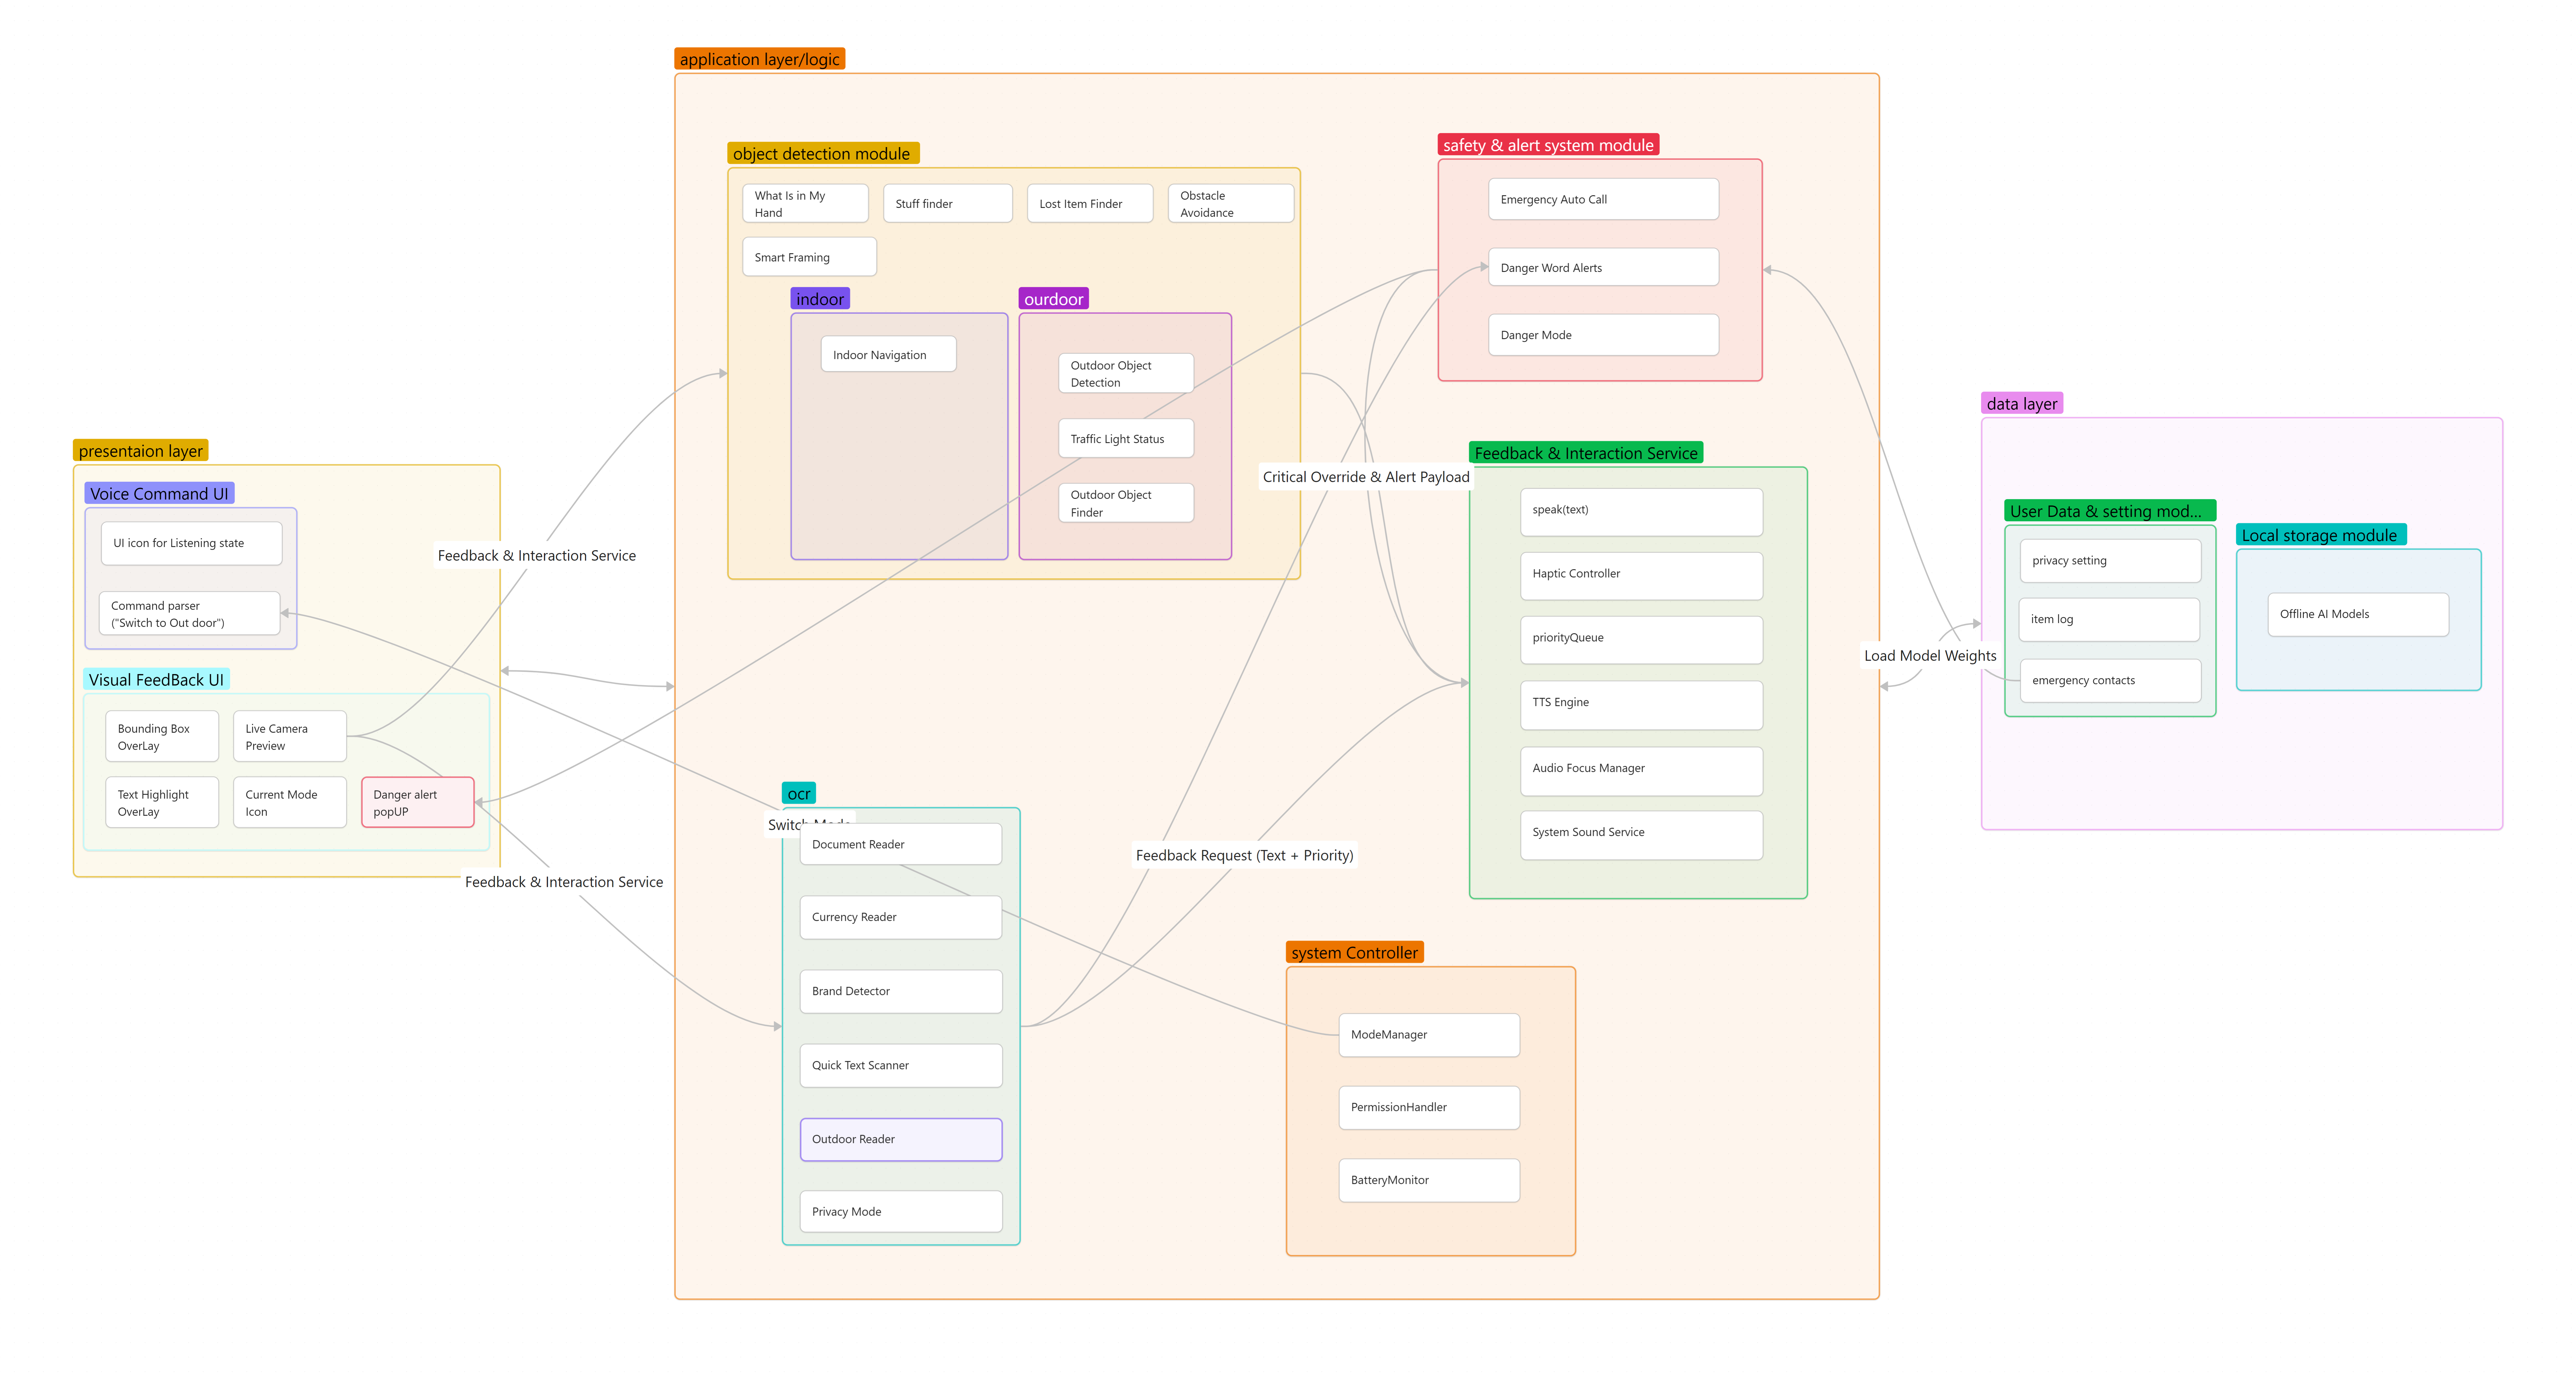
\includegraphics[width=\textwidth,height=0.9\textheight,keepaspectratio]{figures/system_arch.png}
\caption{System Architecture Diagram.}
\label{fig:system-arch}
\end{figure}
\newpage

\section{Class Diagram}

The class diagram illustrates the structural design of the Wareeny system, depicting the key classes, their attributes, methods, and the relationships between them. The diagram captures the core components of the application, including the user interface controllers, AI processing modules, service classes for object detection, OCR, and audio feedback, as well as data models for storing user preferences and detected objects. The relationships shown---such as associations, compositions, and inheritances---demonstrate how the system components collaborate to deliver seamless assistive functionality. This object-oriented design ensures modularity, maintainability, and scalability, allowing for future enhancements and the integration of additional AI models. The class structure is shown in Figure~\ref{fig:class-diagram}.

\begin{figure}[htbp]
\centering
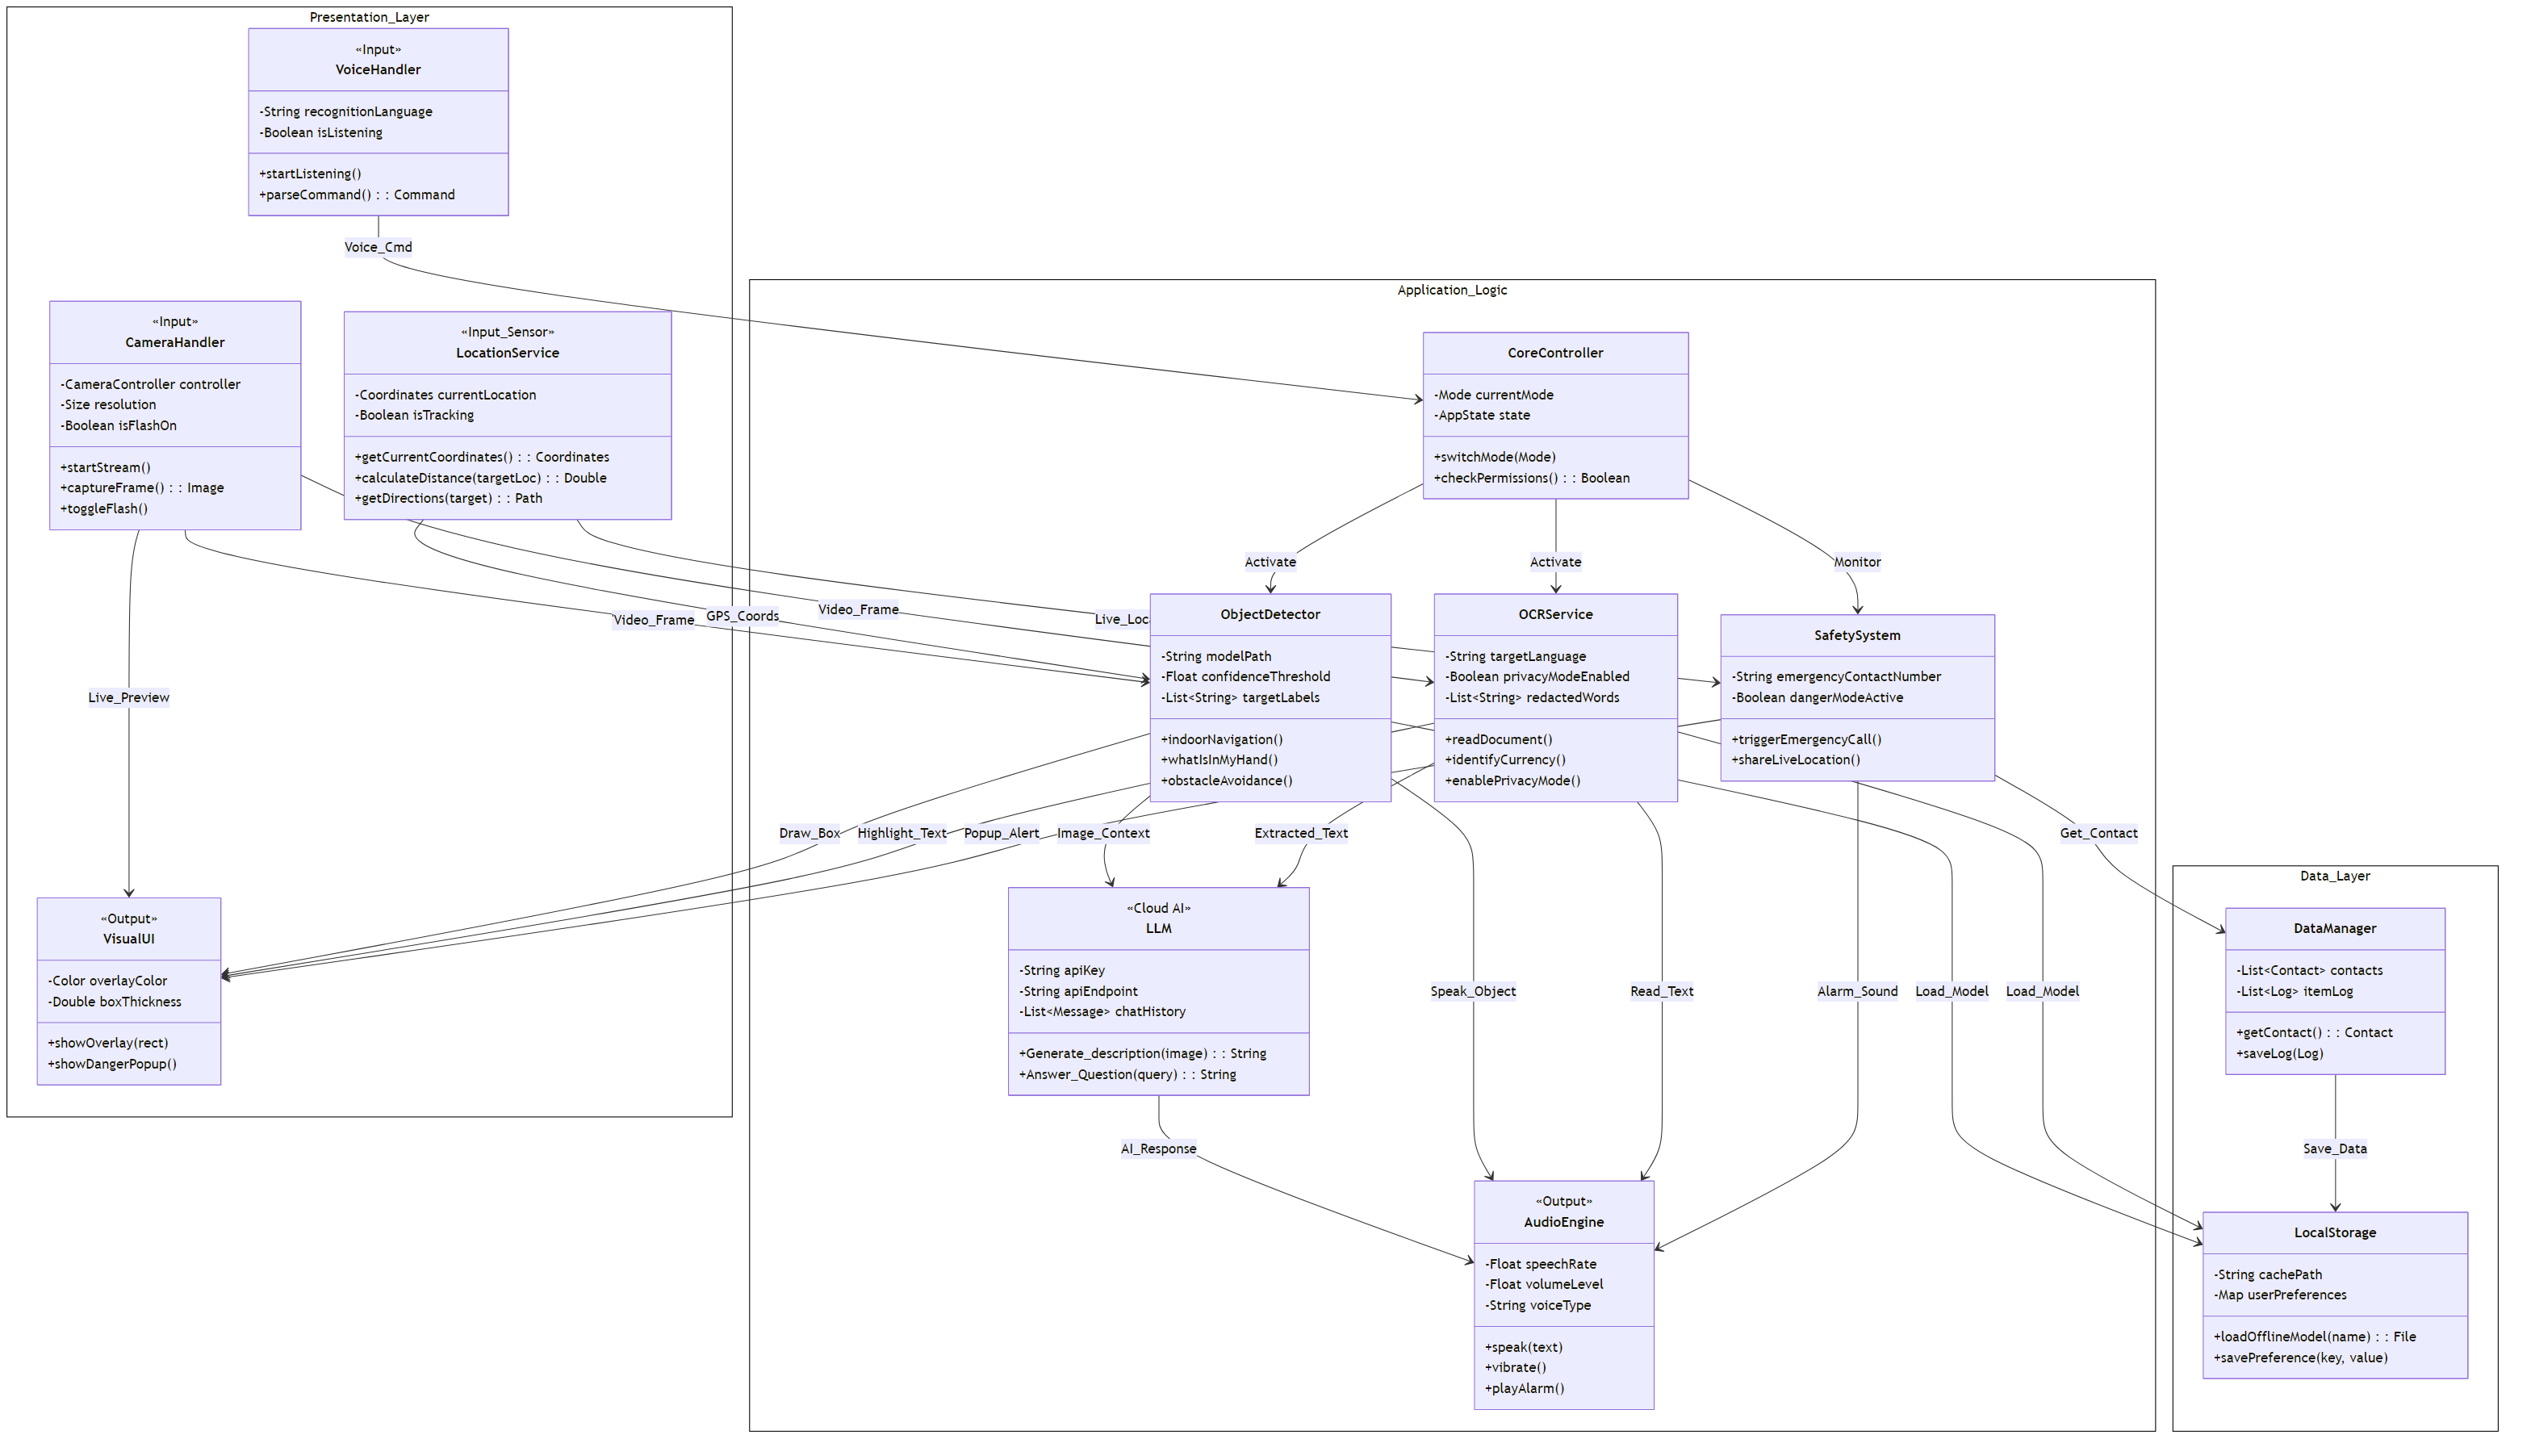
\includegraphics[width=\textwidth,height=0.9\textheight,keepaspectratio]{figures/class_diagram.png}
\caption{Class Diagram.}
\label{fig:class-diagram}
\end{figure}
\newpage

\section{Use Case Diagram}

The use case diagram illustrates the interactions between the user and the Wareeny system, showing the various functionalities available to visually impaired users. Figure~\ref{fig:use-case} presents the system use cases.

\begin{figure}[htbp]
\centering
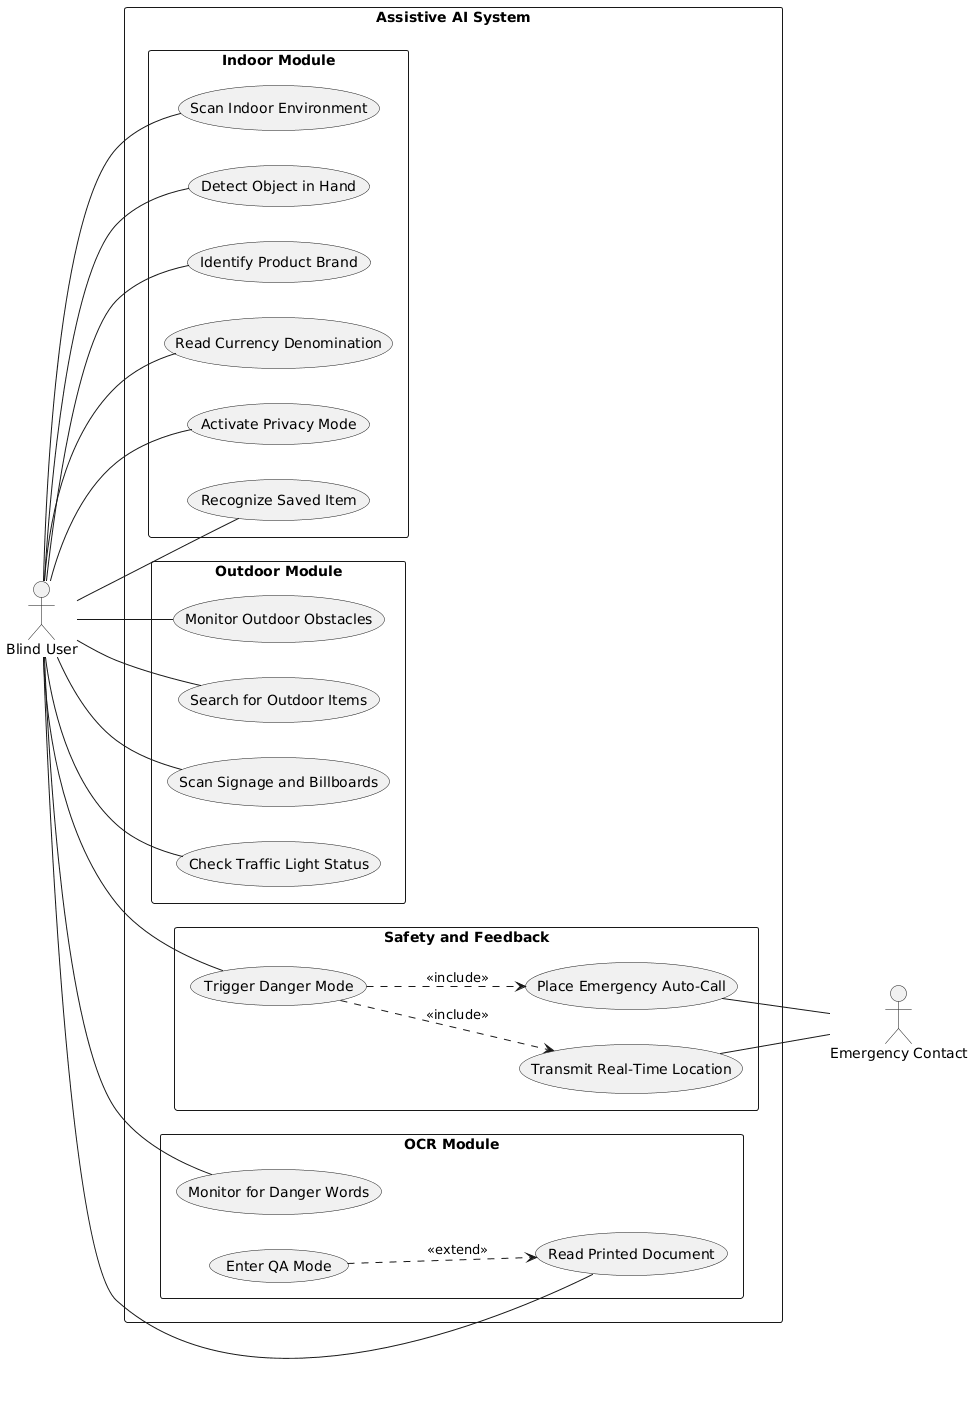
\includegraphics[width=\textwidth,height=0.9\textheight,keepaspectratio]{figures/use_case.png}
\caption{Use Case Diagram.}
\label{fig:use-case}
\end{figure}
\newpage

\section{Sequence Diagrams}

The following sequence diagrams illustrate the flow of interactions for the key features of the Wareeny system.

\subsection{General Flow Diagrams}
The three general flows summarize the dominant interaction patterns of the system: optical character recognition, object detection, and navigation.

\begin{figure}[htbp]
\centering
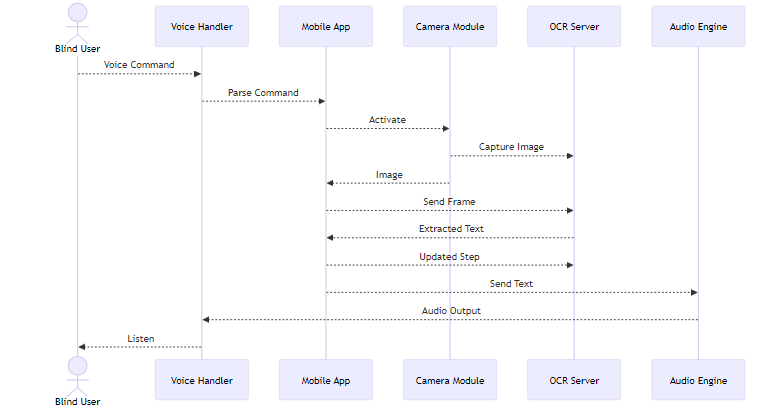
\includegraphics[width=\textwidth,height=0.9\textheight,keepaspectratio]{figures/seq_general_flow_1_ocr.png}
\caption{General Flow 1: OCR Processing.}
\label{fig:seq-genflow1}
\end{figure}

\begin{figure}[htbp]
\centering
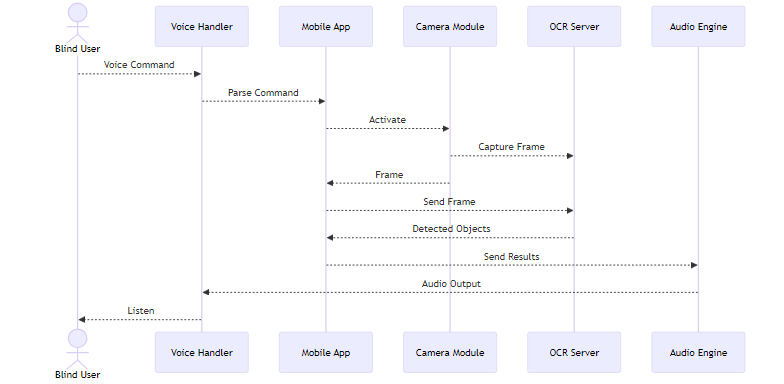
\includegraphics[width=\textwidth,height=0.9\textheight,keepaspectratio]{figures/seq_general_flow_2_object_detection.png}
\caption{General Flow 2: Object Detection Processing.}
\label{fig:seq-genflow2}
\end{figure}

\begin{figure}[htbp]
\centering
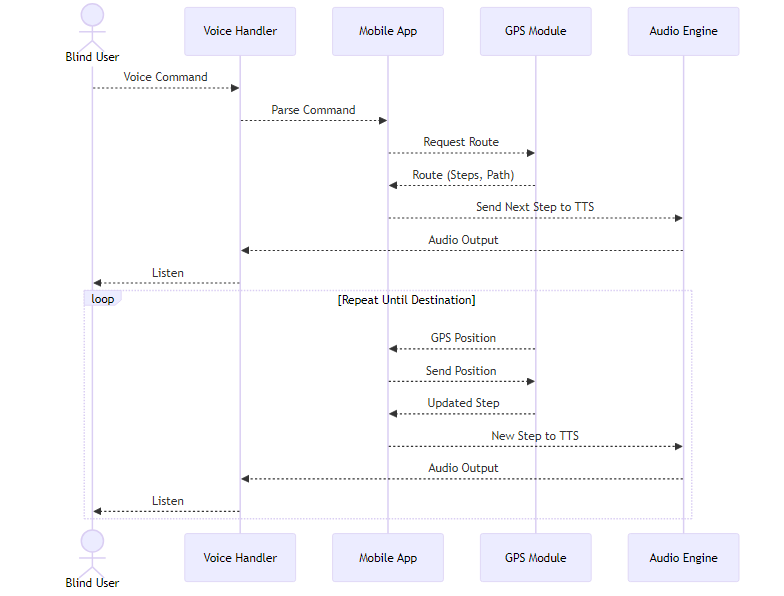
\includegraphics[width=\textwidth,height=0.9\textheight,keepaspectratio]{figures/seq_general_flow_3_navigation.png}
\caption{General Flow 3: Navigation Processing.}
\label{fig:seq-genflow3}
\end{figure}
\newpage

\subsection{Indoor Features}

\begin{figure}[htbp]
\centering
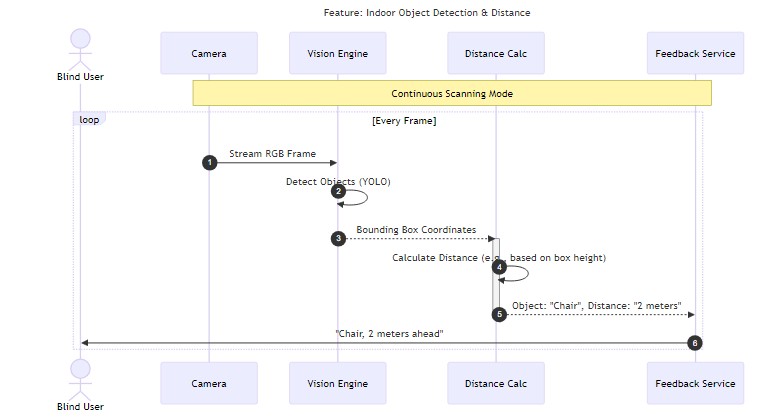
\includegraphics[width=\textwidth,height=0.9\textheight,keepaspectratio]{figures/seq_indoor_object_detection_distance.png}
\caption{Sequence Diagram: Indoor Object Detection and Distance Estimation.}
\label{fig:seq-indoor-objdet}
\end{figure}

\begin{figure}[htbp]
\centering
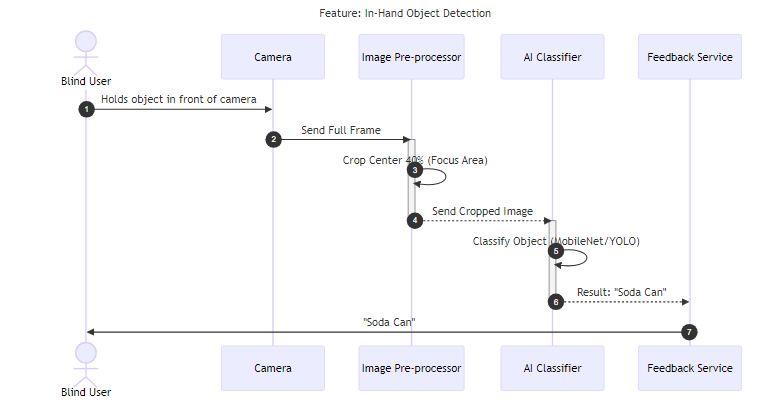
\includegraphics[width=\textwidth,height=0.9\textheight,keepaspectratio]{figures/seq_inhand_object_detection.png}
\caption{Sequence Diagram: In-Hand Object Detection.}
\label{fig:seq-inhand}
\end{figure}

\begin{figure}[htbp]
\centering
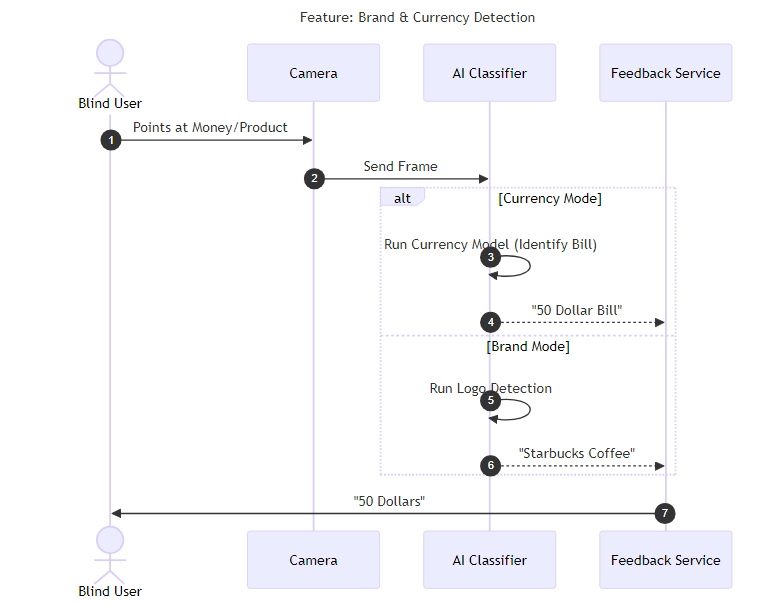
\includegraphics[width=\textwidth,height=0.9\textheight,keepaspectratio]{figures/seq_brand_currency_detection.png}
\caption{Sequence Diagram: Brand and Currency Detection.}
\label{fig:seq-brand-currency}
\end{figure}
\newpage

\subsection{Outdoor Features}

\begin{figure}[htbp]
\centering
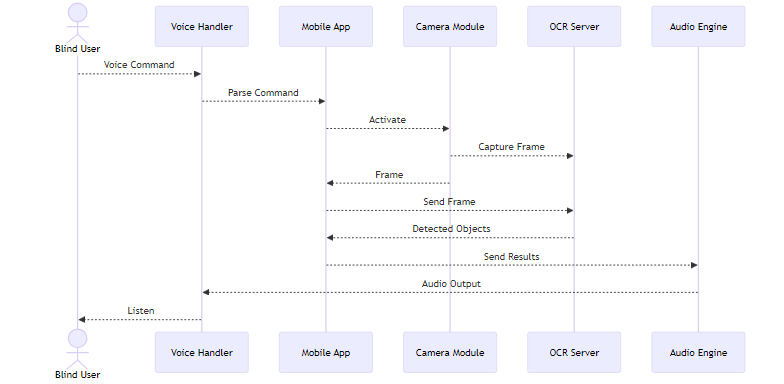
\includegraphics[width=\textwidth,height=0.9\textheight,keepaspectratio]{figures/seq_detect_object_fig2.png}
\caption{Sequence Diagram: Outdoor Object Detection.}
\label{fig:seq-outdoor-objdet}
\end{figure}

\begin{figure}[htbp]
\centering
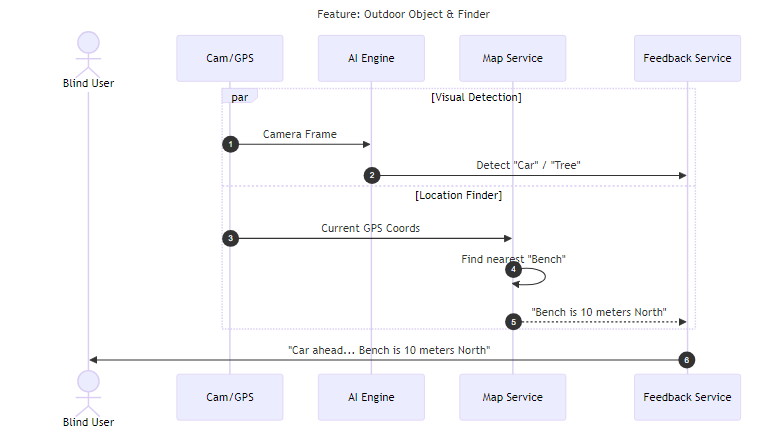
\includegraphics[width=\textwidth,height=0.9\textheight,keepaspectratio]{figures/seq_outdoor_object_finder.png}
\caption{Sequence Diagram: Outdoor Object Finder.}
\label{fig:seq-outdoor-finder}
\end{figure}

\begin{figure}[htbp]
\centering
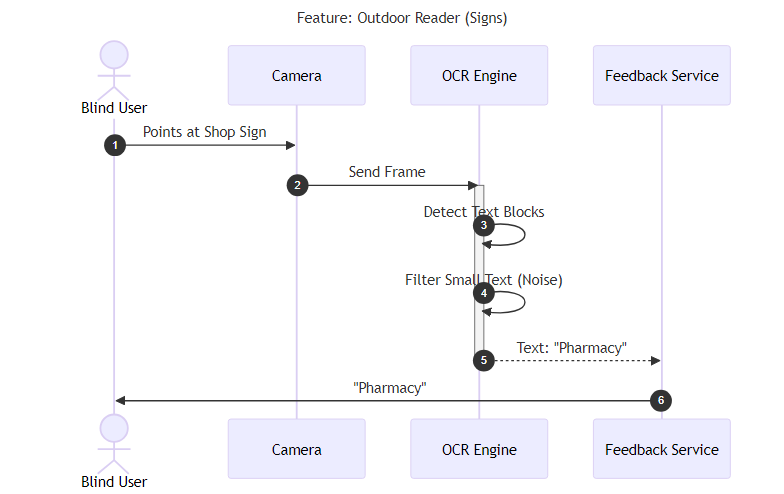
\includegraphics[width=\textwidth,height=0.9\textheight,keepaspectratio]{figures/seq_outdoor_reader_signs.png}
\caption{Sequence Diagram: Outdoor Reader for Signs.}
\label{fig:seq-outdoor-reader}
\end{figure}

\begin{figure}[htbp]
\centering
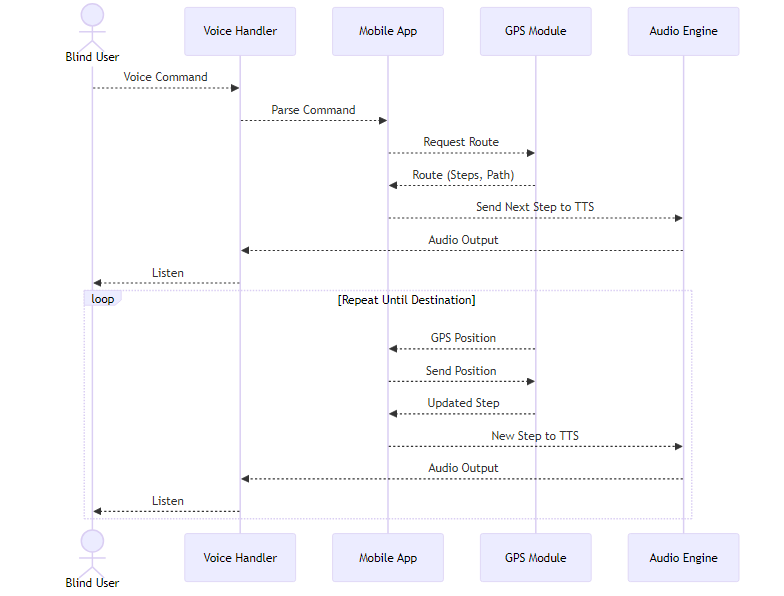
\includegraphics[width=\textwidth,height=0.9\textheight,keepaspectratio]{figures/seq_outdoor_navigation_fig3.png}
\caption{Sequence Diagram: Outdoor Navigation.}
\label{fig:seq-outdoor-nav}
\end{figure}

\begin{figure}[htbp]
\centering
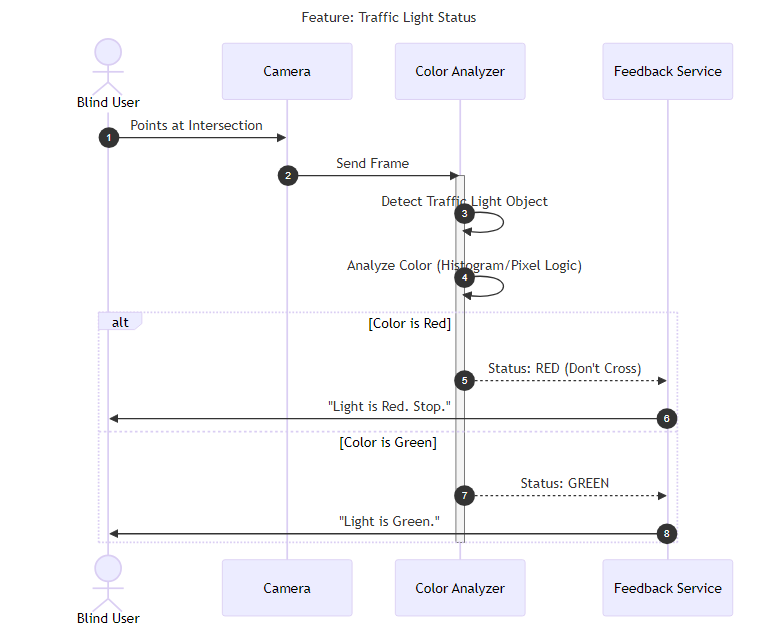
\includegraphics[width=\textwidth,height=0.9\textheight,keepaspectratio]{figures/seq_traffic_light_status.png}
\caption{Sequence Diagram: Traffic Light Status Detection.}
\label{fig:seq-traffic-light}
\end{figure}
\newpage

\subsection{OCR Features}

\begin{figure}[htbp]
\centering
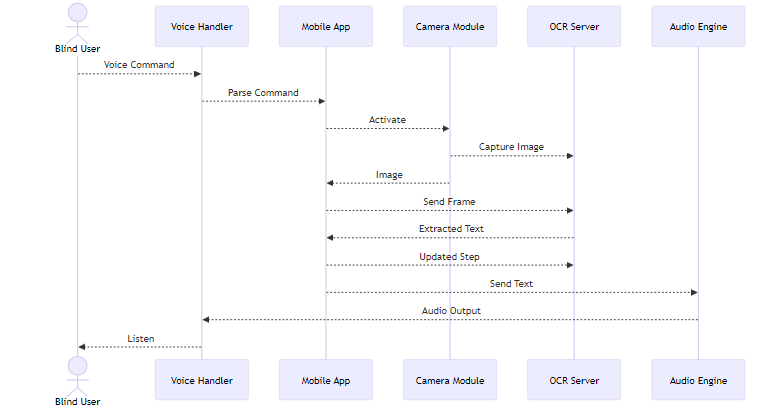
\includegraphics[width=\textwidth,height=0.9\textheight,keepaspectratio]{figures/seq_read_document_fig1.png}
\caption{Sequence Diagram: Read Document.}
\label{fig:seq-read-document}
\end{figure}

\begin{figure}[htbp]
\centering
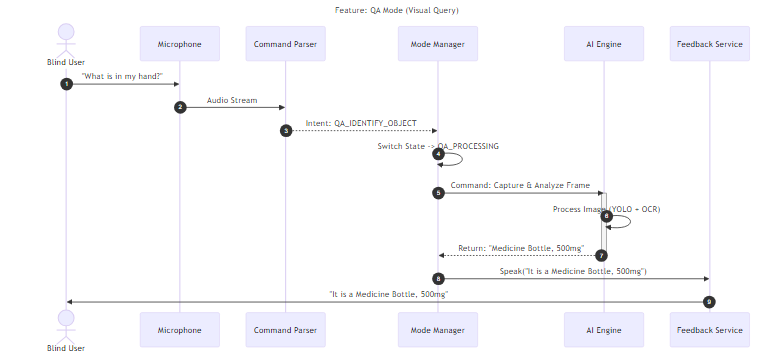
\includegraphics[width=\textwidth,height=0.9\textheight,keepaspectratio]{figures/seq_qa_mode_visual_query.png}
\caption{Sequence Diagram: QA Mode (Visual Query).}
\label{fig:seq-qa-mode}
\end{figure}

\begin{figure}[htbp]
\centering
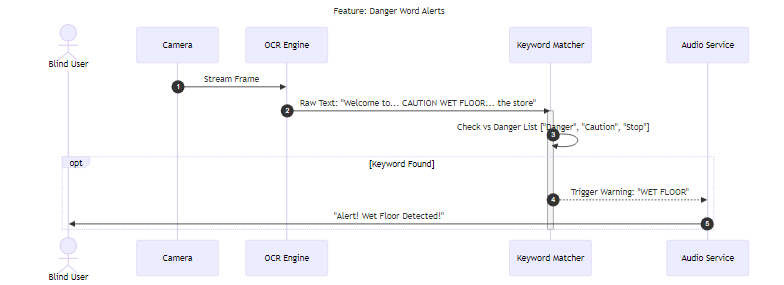
\includegraphics[width=\textwidth,height=0.9\textheight,keepaspectratio]{figures/seq_danger_word_alerts.png}
\caption{Sequence Diagram: Danger Word Alerts.}
\label{fig:seq-danger-words}
\end{figure}
\newpage

\subsection{Safety and Emergency Features}

\begin{figure}[htbp]
\centering
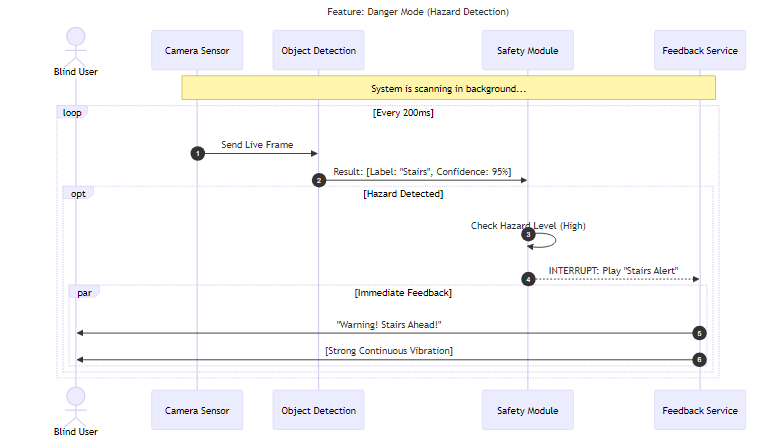
\includegraphics[width=\textwidth,height=0.9\textheight,keepaspectratio]{figures/seq_danger_mode_hazard_detection.png}
\caption{Sequence Diagram: Danger Mode (Hazard Detection).}
\label{fig:seq-danger-mode}
\end{figure}

\begin{figure}[htbp]
\centering
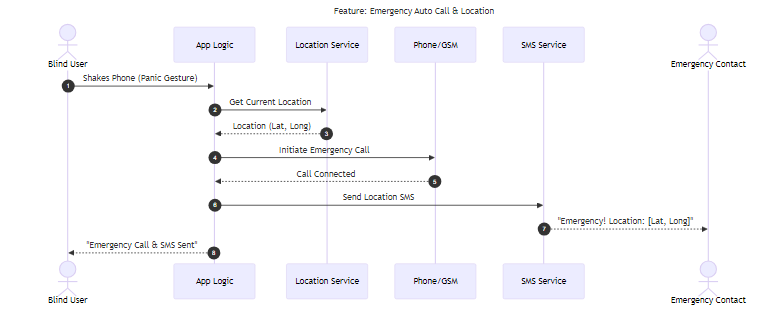
\includegraphics[width=\textwidth,height=0.9\textheight,keepaspectratio]{figures/seq_emergency_auto_call_location.png}
\caption{Sequence Diagram: Emergency Auto Call and Location Sharing.}
\label{fig:seq-emergency-call}
\end{figure}

\begin{figure}[htbp]
\centering
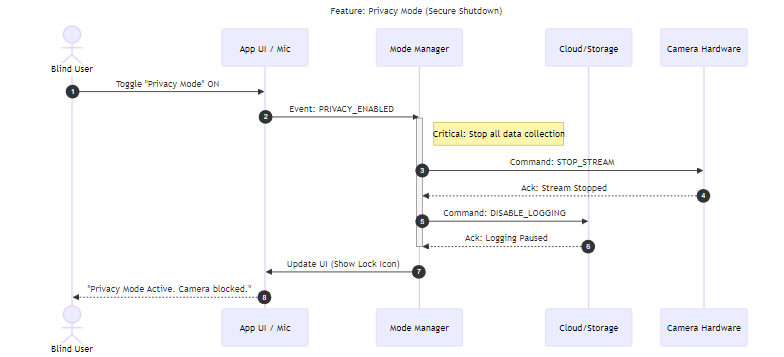
\includegraphics[width=\textwidth,height=0.9\textheight,keepaspectratio]{figures/seq_privacy_mode_secure_shutdown.png}
\caption{Sequence Diagram: Privacy Mode (Secure Shutdown).}
\label{fig:seq-privacy-mode}
\end{figure}
\newpage

\subsection{Audio and Haptics Features}

\begin{figure}[htbp]
\centering
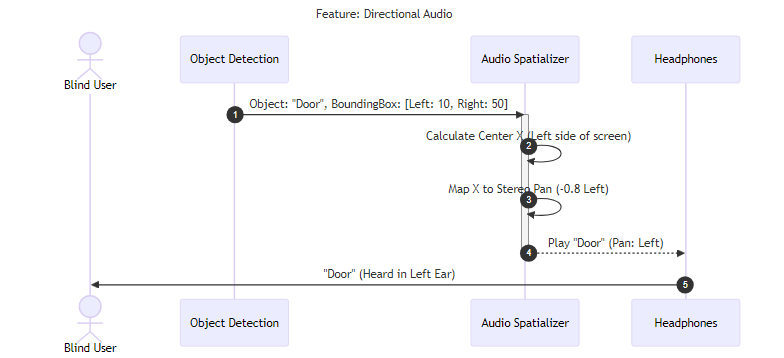
\includegraphics[width=\textwidth,height=0.9\textheight,keepaspectratio]{figures/seq_directional_audio.png}
\caption{Sequence Diagram: Directional Audio.}
\label{fig:seq-directional-audio}
\end{figure}
\newpage

\section{Entity-Relationship Diagram}

The Entity-Relationship Diagram (ERD) illustrates the database schema and data model of the Wareeny system. The diagram depicts the core entities required to store user information, system preferences, detected objects, emergency contacts, and usage history. The relationships between these entities---such as one-to-many and many-to-many associations---demonstrate how data flows and persists throughout the application lifecycle. This relational design ensures efficient data storage, quick retrieval of user-specific information, and maintains the integrity of personal data such as emergency contact details. The ERD serves as the foundation for implementing a robust and scalable database structure that supports all functional requirements of the assistive system. The data model is shown in Figure~\ref{fig:erd}.

\begin{figure}[htbp]
\centering
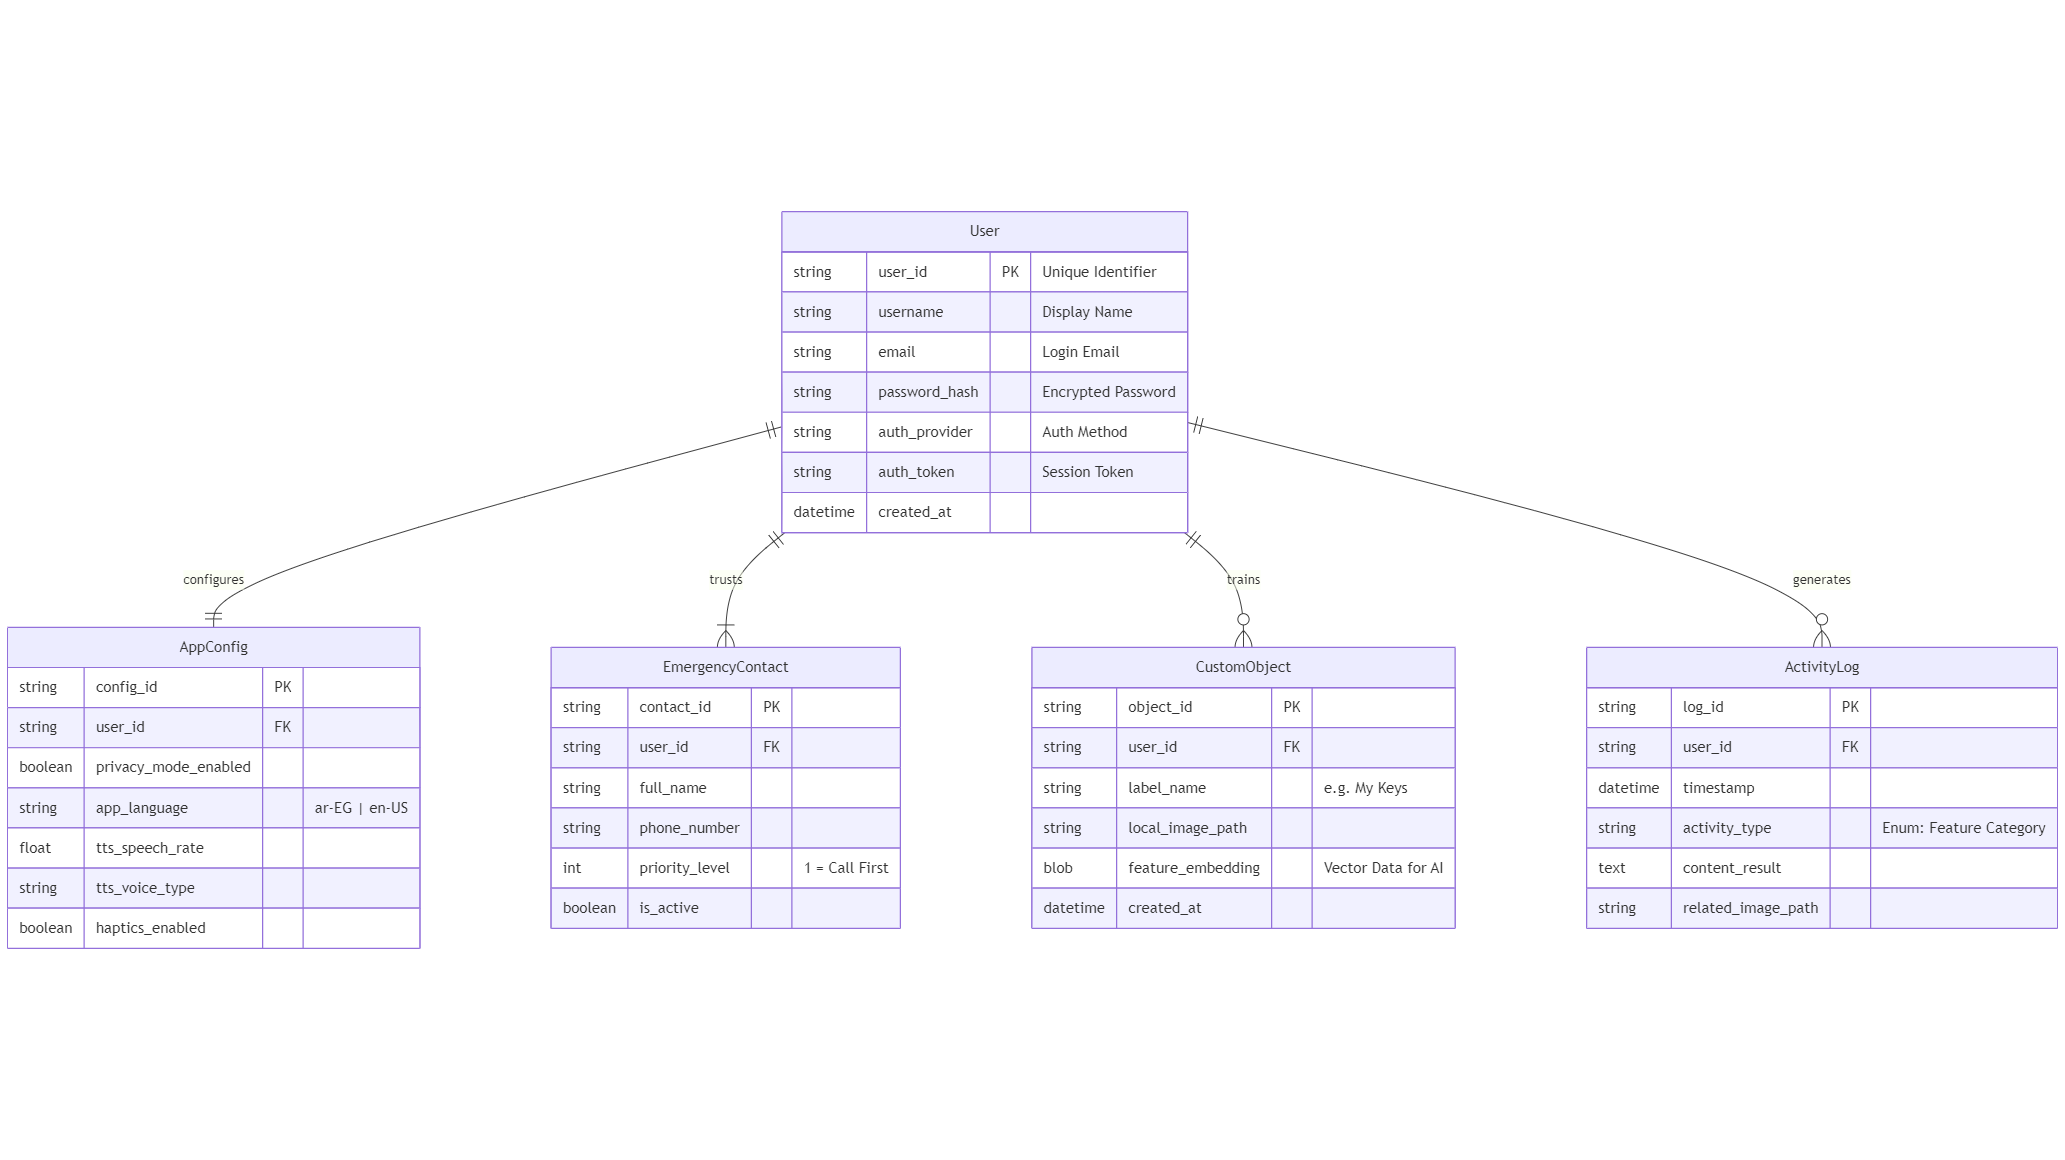
\includegraphics[width=\textwidth,height=0.9\textheight,keepaspectratio]{figures/erd_diagram.png}
\caption{Entity-Relationship Diagram.}
\label{fig:erd}
\end{figure}
\newpage


\chaptercover{4}{Chapter Four}{System Design}
\chapter{System Design}

\section{Introduction}
This chapter presents the design of the Wareeny application as implemented in the project repository. Wareeny is an accessibility-oriented mobile assistant built with Flutter and centred on camera-driven interaction. In its present form the system combines a mode-based interface, a hybrid vision-language reading pipeline, real-time object-detection flows, an on-device Egyptian-pound banknote reader, a background emergency safety subsystem, spoken feedback, haptic alerts, bilingual English--Arabic localization, and persisted user settings. The implemented design is therefore not a conventional form-based mobile application but a sensor-driven assistive system in which perception services and accessibility feedback define the core user experience. Throughout this chapter, design decisions are described as they exist in the codebase, and the boundary between what is fully delivered and what is prepared for future work is stated explicitly so that the account remains accurate and verifiable.

\subsection{Design Orientation}
The design follows four guiding principles. First, interaction must remain usable without sight: every mode is reachable through two-finger gestures, exposes semantic announcements and custom screen-reader actions, and presents large touch targets. Second, high-cost perception logic is isolated behind controllers and service abstractions so that interface widgets stay lightweight and reusable. Third, non-real-time understanding tasks---scanning, reading, scene description, and image questions---are organized around a single shared vision-language architecture rather than isolated feature silos, so that a new understanding feature reuses existing services instead of duplicating inference logic. Fourth, real-time navigation and object-finding behaviour is delegated to local, on-device detection flows in order to keep latency low during active camera use and to avoid streaming a live video feed to any remote service.

\subsection{Implemented Scope}
The implemented application exposes six top-level modes: Home, Navigation, Stuff Finder, Scan, Read, and Settings. Navigation, Stuff Finder, Scan, Read, and Settings are delivered as complete, self-contained interaction paths with dedicated feature controllers. Home is a camera-centred entry surface rather than a full feature screen. Internally, the vision-language task model defines four tasks---scan, read, scene description, and ask-image---of which scan and read are fully wired to finished screens, while scene description and ask-image exist as service-level tasks ready to be surfaced. The Scan mode consolidates what were previously separate in-hand, currency, and brand concepts into a single one-tap ``identify whatever the camera is pointed at'' interaction, with Egyptian-pound money reading handled ahead of the language model by a dedicated on-device banknote detector.

In addition to the visible carousel modes, the system runs an active background Emergency and Safety subsystem. This module remains armed during the application runtime, listening to accelerometer sensor data to detect user-shake events, enabling danger triggers without requiring visual search or manual screen clicks.

\section{Development Tools and Technologies}
\subsection{Flutter and Dart}
Flutter and Dart form the foundation of the application. Flutter provides the cross-platform widget system, theming model, animation support, semantics integration, and localization hooks used across the project, while Dart is used for screen composition, stateful feature controllers, dependency registration, bridge abstractions, and AI-service orchestration. This combination suits Wareeny because it supports rapid user-interface iteration while still allowing native platform integration through method and event channels where lower-level performance is required, such as haptic playback and the native object-detection runtime.

\subsection{Visual Input and Camera Capture}
The application uses two distinct visual-input paths, and the split is architecturally deliberate. For reading and scanning, the \texttt{camera} package opens the rear camera, shows a live preview, and captures a single still image on demand; the scan path requests a high-resolution preset specifically so that small printed banknote numerals remain legible. For navigation and stuff-finder, the \texttt{ultralytics\_yolo} package provides a streaming camera view bound directly to YOLO inference. Reading and scanning need a deliberate still frame for interpretation, whereas navigation and object finding require continuous frame analysis; using the right capture model for each avoids paying streaming costs where a single frame suffices.

\subsection{Vision-Language Reading Stack}
The reading and scanning subsystem is built around the \texttt{VlmAssistant}, the single entry point that accepts an image path and a task definition and returns a stream of spoken-text events. It routes each request through a \texttt{ModelRouter}, a pure policy object that returns an ordered list of providers to try for a given task. Two providers implement the common \texttt{VlmProvider} contract: a \texttt{LocalVlmProvider} backed by an on-device vision-language runtime, and a \texttt{CloudVlmProvider} backed by a self-hosted Gemma backend. The assistant walks the providers in order, streams tokens from the first that can serve the request, and falls back to the next tier only when a provider declares itself unavailable before producing output. The task model defines a dedicated \texttt{currency} task; in the current build this task is served by the same vision-language pipeline as the other understanding tasks, while the \texttt{VlmProvider} contract is intentionally shaped so that a specialized on-device banknote provider can later be registered ahead of the language model without changing any screen or controller. Prompt construction is centralized in \texttt{VlmPrompts}, where each task carries a tuned, spoken-style system prompt, so that scan and read produce appropriately different behaviour while preserving a consistent assistive tone. A \texttt{SpeechQueue} receives streamed sentence-sized chunks and speaks them sequentially, allowing audio to begin before the full response has been generated.

\subsection{Real-Time Object Detection Stack}
Real-time detection is abstracted behind the \texttt{ObjectDetectionSource} interface. The concrete implementation in active use is \texttt{UltralyticsYoloDetectionSource}, which emits streaming detection frames and selects bundled model assets according to the active feature mode---a general YOLOv8n detector for navigation and a custom-trained YOLOv8n detector for stuff finding. Detection frames are normalized through a \texttt{DetectionCoordinateMapper}, which corrects for sensor rotation and mirroring, before higher-level logic such as the \texttt{NavigationRiskEngine} or the \texttt{StuffFinderController} interprets them. The same single-stage detection approach is the basis on which a dedicated single-shot Egyptian-pound banknote detector is planned: it would run a custom-trained YOLOv8n banknote model on individual captured stills rather than on a live stream, since money reading is tap-to-capture rather than continuous. This detector is not yet bundled in the current build, and currency reading is presently handled by the vision-language pipeline described above.

\subsection{Localization, Speech, and Preference Persistence}
Flutter localization delegates and a custom \texttt{AppLocalizations} class provide bilingual English and Arabic user-facing strings. Audio output is handled by the \texttt{AudioHapticsBridge}, which wraps \texttt{flutter\_tts}, prefers an Egyptian-Arabic (\texttt{ar-EG}) voice when one is installed, and configures speech rate, pitch, and completion callbacks; the same bridge also exposes categorized haptic signals. Persisted user settings are managed by the \texttt{SettingsController}, which stores the locale, speech rate, and haptics preference in \texttt{SharedPreferences}. This gives the application a lightweight persistence model suitable for personalization without introducing premature relational-database complexity.

\section{Architectural Evolution: Detection-and-OCR versus a Vision-Language Pipeline}
The current architecture is the result of a deliberate design pivot made during development. The initial plan followed the conventional assistive-application pattern: a YOLO-family object detector would handle every recognition task, and Google ML Kit would handle every text-reading task. This combination is fast and fully on-device, but as the requirements matured it proved structurally mismatched with the accessibility goals of the project, and the understanding layer was re-centred on a vision-language model (the self-hosted Gemma family) instead.

\subsection{Motivation for the Pivot}
Three limitations drove the change. First, a supervised detector such as YOLO can only recognize the finite set of classes it was trained on; any object outside that set is simply invisible to it, which is unacceptable for an assistant whose users point the camera at arbitrary, unpredictable objects. A vision-language model, by contrast, performs strong zero-shot recognition and can describe objects it was never explicitly trained to detect. Second, a classical OCR engine such as ML Kit emits a flat, verbatim character stream with no understanding of layout, salience, or intent; it cannot distinguish a heading from a footer, cannot answer a question about a document, and tends to overwhelm a blind user with undifferentiated text. Mekonnen et al.\ (2025) demonstrate this ceiling concretely: a state-of-the-art offline assistive system using Tesseract OCR achieves 89.7\% word accuracy on clean printed English text under optimal lighting, but this falls to 73.9\% at normal walking speed, and the engine provides no support for Arabic script or semantic understanding of what it reads [20]. A vision-language model reads text \emph{in context}, reporting only the facts that matter in a natural spoken style, and handles Arabic and mixed-language documents without a separate language-specific engine. Third, a detector produces bounding boxes, not answers: it cannot support Visual Question Answering (VQA), which the literature (Huh et al., 2024 [1]) identifies as the interaction blind users most prefer. These three gaps---closed-set recognition, context-free OCR, and the absence of reasoning---together motivated consolidating the understanding tasks behind a single vision-language pipeline, while retaining YOLOv8n only for the latency-critical, closed-set tasks (navigation and stuff finding) where its speed is an asset and its fixed class set is acceptable.

\subsection{Comparative Justification}
Table~\ref{tab:vlm-vs-classical} preserves the conceptual trade-off between the two design directions, while Table~\ref{tab:vlm-stats} adds representative published statistics for speed, accuracy, and user outcome. The values are included to justify the architectural decision and are drawn from the literature reviewed earlier rather than from direct benchmarking of the implemented repository.

\begin{table}[H]
\centering
\caption{Classical Detection/OCR versus the Vision-Language Pipeline for Accessibility}
\label{tab:vlm-vs-classical}
\begin{tabularx}{\textwidth}{|>{\raggedright\arraybackslash}p{0.22\textwidth}|>{\raggedright\arraybackslash}X|>{\raggedright\arraybackslash}X|}
\hline
\textbf{Dimension} & \textbf{YOLO / ML Kit (initial plan)} & \textbf{Vision-Language Model (adopted)} \\
\hline
Object recognition scope & Closed-set: only trained classes (e.g.\ 80 COCO classes [11]); effectively 0\% recall on any untrained object & Open-vocabulary, zero-shot: recognizes and describes objects outside any fixed label set \\
\hline
Text reading & Verbatim OCR; no layout or salience awareness; reads page furniture indiscriminately & Context-aware reading; distinguishes body from headers/footers and reports only salient content \\
\hline
Reasoning / interaction & Bounding boxes and class labels only; no question answering & Supports Visual Question Answering (VQA) and multi-turn queries about the image \\
\hline
Output for blind users & Raw labels and full text dumps, prone to cognitive overload & Concise, natural-language spoken answers tuned to user intent \\
\hline
On-device latency & Very low; real-time streaming ($\sim$15 FPS, YOLOv8n [15]) & Higher per-query latency; suited to deliberate, tap-to-capture tasks \\
\hline
Role in final design & Retained for latency-critical, closed-set tasks (navigation, stuff finding) & Adopted for all open-ended understanding (scan, read, scene, VQA) \\
\hline
\end{tabularx}
\end{table}

\begin{table}[H]
\centering
\caption{Numerical Performance Comparison: Classical Pipeline vs.\ Wareeny's Hybrid Approach}
\label{tab:vlm-stats}
\begin{tabularx}{\textwidth}{|>{\raggedright\arraybackslash}X|C{2.2cm}|C{2.6cm}|C{1.4cm}|C{1.5cm}|}
\hline
\textbf{Metric} & \textbf{Classical Pipeline} & \textbf{Wareeny Approach} & \textbf{Gain} & \textbf{Ref.} \\
\hline
Navigation speed (FPS) & 12.8--15.2 & 12.8--15.2 (preserved) & --- & [4], [5] \\
\hline
OCR accuracy -- Arabic handwriting (\%) & 68 & 89 (VLM contextual) & +21 pp & [2] \\
\hline
OCR accuracy -- dynamic scene (\%) & 73.9 & No fixed ceiling & --- & [20] \\
\hline
Currency recognition -- controlled (\%) & 72 & 94 (localized model) & +22 pp & [3] \\
\hline
Currency recognition -- worn notes (\%) & 72 & 87 (localized model) & +15 pp & [3] \\
\hline
User task completion vs.\ static captioning & baseline & +40\% & +40\% & [1] \\
\hline
\end{tabularx}
\end{table}

Table~\ref{tab:vlm-stats} therefore compares the two directions more directly. The classical pipeline remains strong in one area: speed. That is why Wareeny keeps detector-based processing for navigation and preserves the real-time 12.8--15.2 FPS operating range reported in the literature [4], [5]. Where the adopted Wareeny design improves is in understanding quality and user usefulness. Instead of relying on an OCR-only path whose robustness can fall to 68\% on challenging Arabic text [2], the system shifts reading into a contextual VLM pipeline, motivated by Arabic-reading results that rise from 68\% to 89\%, or by 21 percentage points, when moving beyond the generic OCR baseline [2]. Instead of depending on generalized visual models for region-specific tasks, the architecture leaves room for localized Egyptian-currency recognition, where published results rise from 72\% to 94\% in controlled conditions [3]. Most importantly, the interaction model aligns with evidence that interactive VQA-style assistance can improve task completion by 40\% over static captioning [1]. This is the numerical reason the project adopts a hybrid architecture rather than a purely classical one.

\section{System Architecture}
The application is organized into five cooperating layers: presentation, application control, AI services, backend integration, and persistence. Dependencies flow downward---screens depend on controllers, controllers depend on shared services, and services depend on bridges and providers---while no lower layer reaches back into a higher one. Cross-cutting dependencies are wired once during startup by a \texttt{ServiceRegistry} and exposed to the widget tree through an inherited \texttt{AppScope}, which keeps construction logic out of individual screens.

\subsection{Presentation Layer}
The presentation layer consists of the \texttt{NavigationShell} and the feature screens it hosts: \texttt{ReadScreen}, \texttt{ScanScreen}, \texttt{NavigationScreen}, \texttt{StuffFinderScreen}, and \texttt{SettingsScreen}. Reusable widgets---\texttt{CameraTopBar}, \texttt{ModeCarouselBar}, \texttt{TwoFingerSwipeDetector}, status pills, side-action controls, and mode-specific overlays---provide a consistent visual language across modes. The presentation layer is deliberately thin: it captures gestures, renders current state, and delegates all feature behaviour to dedicated controllers.

\subsection{Application Control Layer}
The application control layer contains the stateful controllers that coordinate each feature. The \texttt{VlmReadController} drives both Scan and Read: it manages the capture-to-speech state machine, token streaming, the ``thinking'' cue that covers first-token latency, and---for Read---the stop, repeat, skip, and cancel controls. The \texttt{NavigationController} consumes streaming detection frames, applies geometric risk rules with confirmation windows and cooldowns, and triggers directional speech and haptics. The \texttt{StuffFinderController} manages target selection, detector startup, match filtering, and cooldown-gated spoken announcements. The \texttt{SettingsController} manages persistent configuration and notifies the interface whenever the locale, speech rate, or haptics preference changes.

\subsection{AI Service Layer}
The AI service layer holds the reusable logic beneath the controllers. On the vision-language side it includes the \texttt{VlmAssistant}, the \texttt{ModelRouter}, the centralized \texttt{VlmPrompts}, and the three provider implementations. On the detection side it includes the \texttt{ObjectDetectionSource} abstraction, the \texttt{DetectionCoordinateMapper}, the detection data models, the \texttt{BanknoteDetector}, and the navigation geometry and risk scoring in \texttt{NavigationRiskEngine}. Keeping this logic in a shared layer is what allows new assistive flows to be added by reusing services rather than duplicating inference inside screens.

\subsection{Backend Integration Layer}
The backend integration layer is represented by the \texttt{CloudVlmProvider}. This provider probes a remote \texttt{/health} endpoint, downscales and re-encodes the captured image off the main isolate to bound upload size and first-token latency, sends a multimodal request to \texttt{/vlm/generate}, and parses a Server-Sent Events stream so that tokens can be spoken as they arrive. It also recognizes a streamed error payload from the backend and converts it into an ``unavailable'' signal so that the assistant can fall back or report cleanly rather than appearing to produce an empty reading. The backend service itself is external to this repository, but the client-side contract---endpoints, request shape, and streaming format---is fully encoded in the application.

\subsection{Persistence Layer}
The persistence layer is intentionally lightweight. \texttt{SharedPreferences} stores the long-lived personalization keys, while all transient perception state---streamed reading text, the active speech queue, the latest detection frame, the current navigation assessment, and the selected stuff-finder target---is held in controller memory and is meaningful only within the current session. Wareeny therefore uses a mixed persistence model by design: durable key-value settings for personalization and in-memory runtime objects for live camera sessions.

\section{Application Map}
\subsection{Startup and Home Flow}
Application startup begins in a \texttt{bootstrap} routine, which initializes the widget binding, loads environment configuration through \texttt{AppConfig}, builds the \texttt{ServiceRegistry} asynchronously (restoring settings from \texttt{SharedPreferences} along the way), and eagerly initializes text-to-speech so that the first spoken prompt is not delayed. The user is then placed into the \texttt{NavigationShell}. From the shell, Home acts as a camera-centred entry surface rather than a form-driven dashboard, and the user moves across modes through the carousel or two-finger horizontal swipes.

\subsection{Navigation Mode Flow}
In Navigation mode the shell opens \texttt{NavigationScreen}, instantiates a \texttt{NavigationController}, and connects it to a YOLO streaming view. Detection frames are oriented, passed into the \texttt{NavigationRiskEngine}, and converted into caution, danger, low-light, or path-clear feedback. The risk engine evaluates each object against a forward path region, weighing confidence, box area, and overlap with the path; the controller then stabilizes that signal through short confirmation windows (shorter for danger than for caution) and rate-limits output with separate speech and haptic cooldowns, so that warnings are timely without becoming repetitive. Spoken guidance is issued in Egyptian Arabic---for example, a left-offset obstacle prompts the user to step right and a close frontal obstacle prompts a stop---and a path-clear confirmation is spoken only after several consecutive clear frames. Indoor and outdoor submodes are present in the interface and currently share the same detection pipeline, which leaves room for later environment-specific tuning without restructuring the screen.

\subsection{Stuff Finder Mode Flow}
In Stuff Finder mode the user first selects a target from a picker that merges custom assistive classes---such as wallet, glasses, and keys---with standard COCO object classes. Once a target is chosen, the \texttt{StuffFinderController} starts the detector, selects the appropriate custom model path, receives streaming frames, filters detections down to the selected label, and updates a status indicator with the current match state. Spoken feedback announces the chosen target and the presence of matches, while a cooldown prevents repetitive announcements.

\subsection{Scan Mode Flow}
Scan mode is the application's one-tap identification path, implemented by \texttt{ScanScreen} over the shared \texttt{VlmReadController}. A single tap captures a high-resolution still, which is submitted as a scan task. The \texttt{ModelRouter} prefers the on-device vision-language model for privacy and offline use and falls back to the self-hosted backend when the local model is unavailable and the network is reachable. The model identifies the subject as a packaged product read off its label, a sign or document reduced to the one or two facts that matter, a banknote whose denomination is reported, or a plain object. Because Scan targets blind users, it offers no playback controls; instead it exposes a ``repeat result'' gesture and screen-reader action so a missed answer can be heard again. The routing layer is structured so that a dedicated on-device banknote detector can later be inserted ahead of the language model for this path, improving denomination accuracy and enabling fully offline money reading; that detector is reserved for future work.

\subsection{Read Mode Flow}
In Read mode the user captures a still image of a document, which is submitted as a read task. Routing prefers the on-device vision-language model for privacy and offline use and falls back to the self-hosted backend when the local model is unavailable and the network is reachable. The read prompt instructs the model to read the main body faithfully and in order while skipping page furniture such as headers, footers, and page numbers, so the result is a faithful reading rather than a summary. Streamed text is buffered into speakable sentences and spoken progressively, and the screen keeps stop, repeat, skip, and cancel controls available until the speech queue has fully drained, because generation typically outruns playback.

\subsection{Settings Flow}
Settings mode operates without the live camera and provides language, speech-rate, and haptics controls presented as glass-style configuration cards in the same visual language as the rest of the application. Every change is written to \texttt{SharedPreferences} immediately and propagated through the widget tree, so subsequent launches reproduce the user's preferred accessibility profile.

\subsection{Emergency and Safety Flow}
The safety flow is managed as an active background service by the \texttt{EmergencyController}. Armed on application bootstrap, it listens to acceleration events via the \texttt{ShakeDetectorService}. When a qualifying device shake is detected, the controller halts active presentation, triggers a semantic announcement, and pushes the modal \texttt{EmergencyOverlay} onto the screen. This starts a 5-second countdown timer. If the user does not tap the cancel target, the controller executes a multi-stage emergency dispatch: it (1) fetches device GPS coordinates via the \texttt{LocationService}, (2) automatically dials the primary emergency contact via \texttt{flutter\_phone\_direct\_caller}, (3) silently formats and transmits an SMS message containing the location link natively (Android) or opens a prepared draft (iOS), and (4) invokes a WhatsApp intent with a pre-filled safety message for redundant contact warning.

\section{UI/UX Design}
\subsection{Accessibility Interaction Model}
The interaction model is designed around non-visual control. Two-finger horizontal swipes switch top-level modes, and feature screens attach custom semantics actions so that screen-reader users can jump directly to any other mode or invoke feature actions without relying on visual controls. Live status values are exposed as semantic live regions, and major mode changes are announced aloud. Accessibility is therefore not an added layer over a visual interface; it is the primary navigation model of the system.

\subsection{Visual Design Language}
The visual layer uses a dark full-screen camera background with glassmorphism overlays, electric-green highlights, rounded cards, and centrally placed status elements, applied consistently across the top bar, mode carousel, settings cards, reading controls, and status pills. Even though the target user may not depend on vision, a clean and stable visual layout remains valuable for caregivers, demonstrations, testing, and hybrid low-vision use.

\subsection{Screen Designs}
Figures~\ref{fig:ui-home}--\ref{fig:ui-settings} present the principal screen designs of the implemented application.

\begin{figure}[ht]
\centering
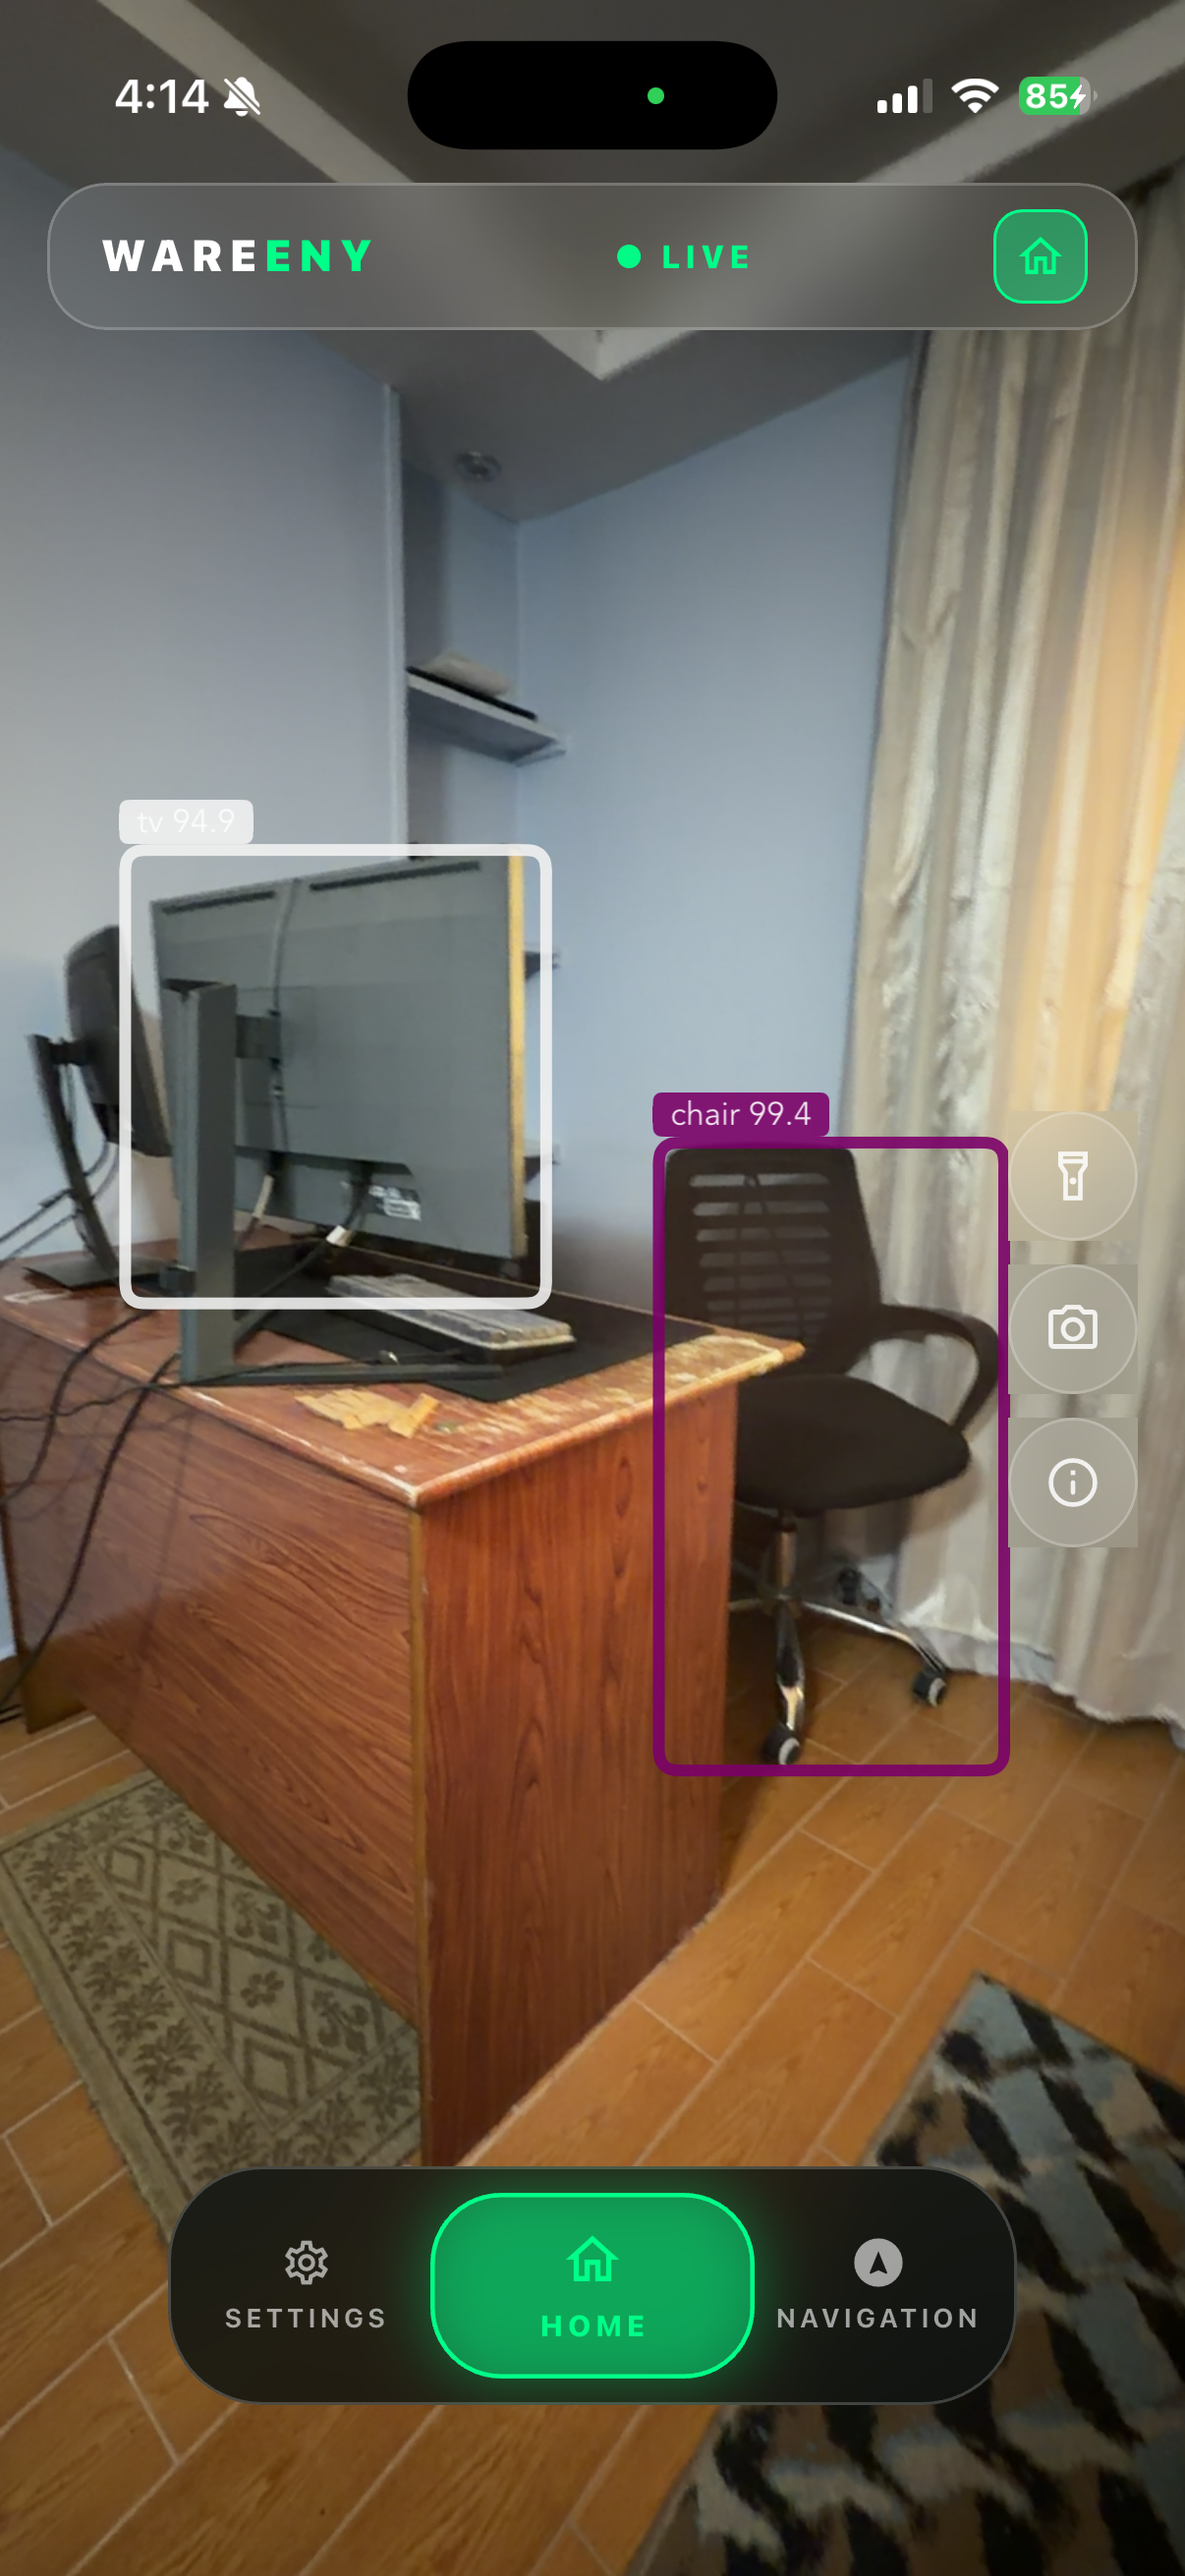
\includegraphics[width=0.32\textwidth]{figures/ui_home.png}
\caption{Home and Scan entry surface with the camera preview, mode carousel, and top status bar.}
\label{fig:ui-home}
\end{figure}

\begin{figure}[ht]
\centering
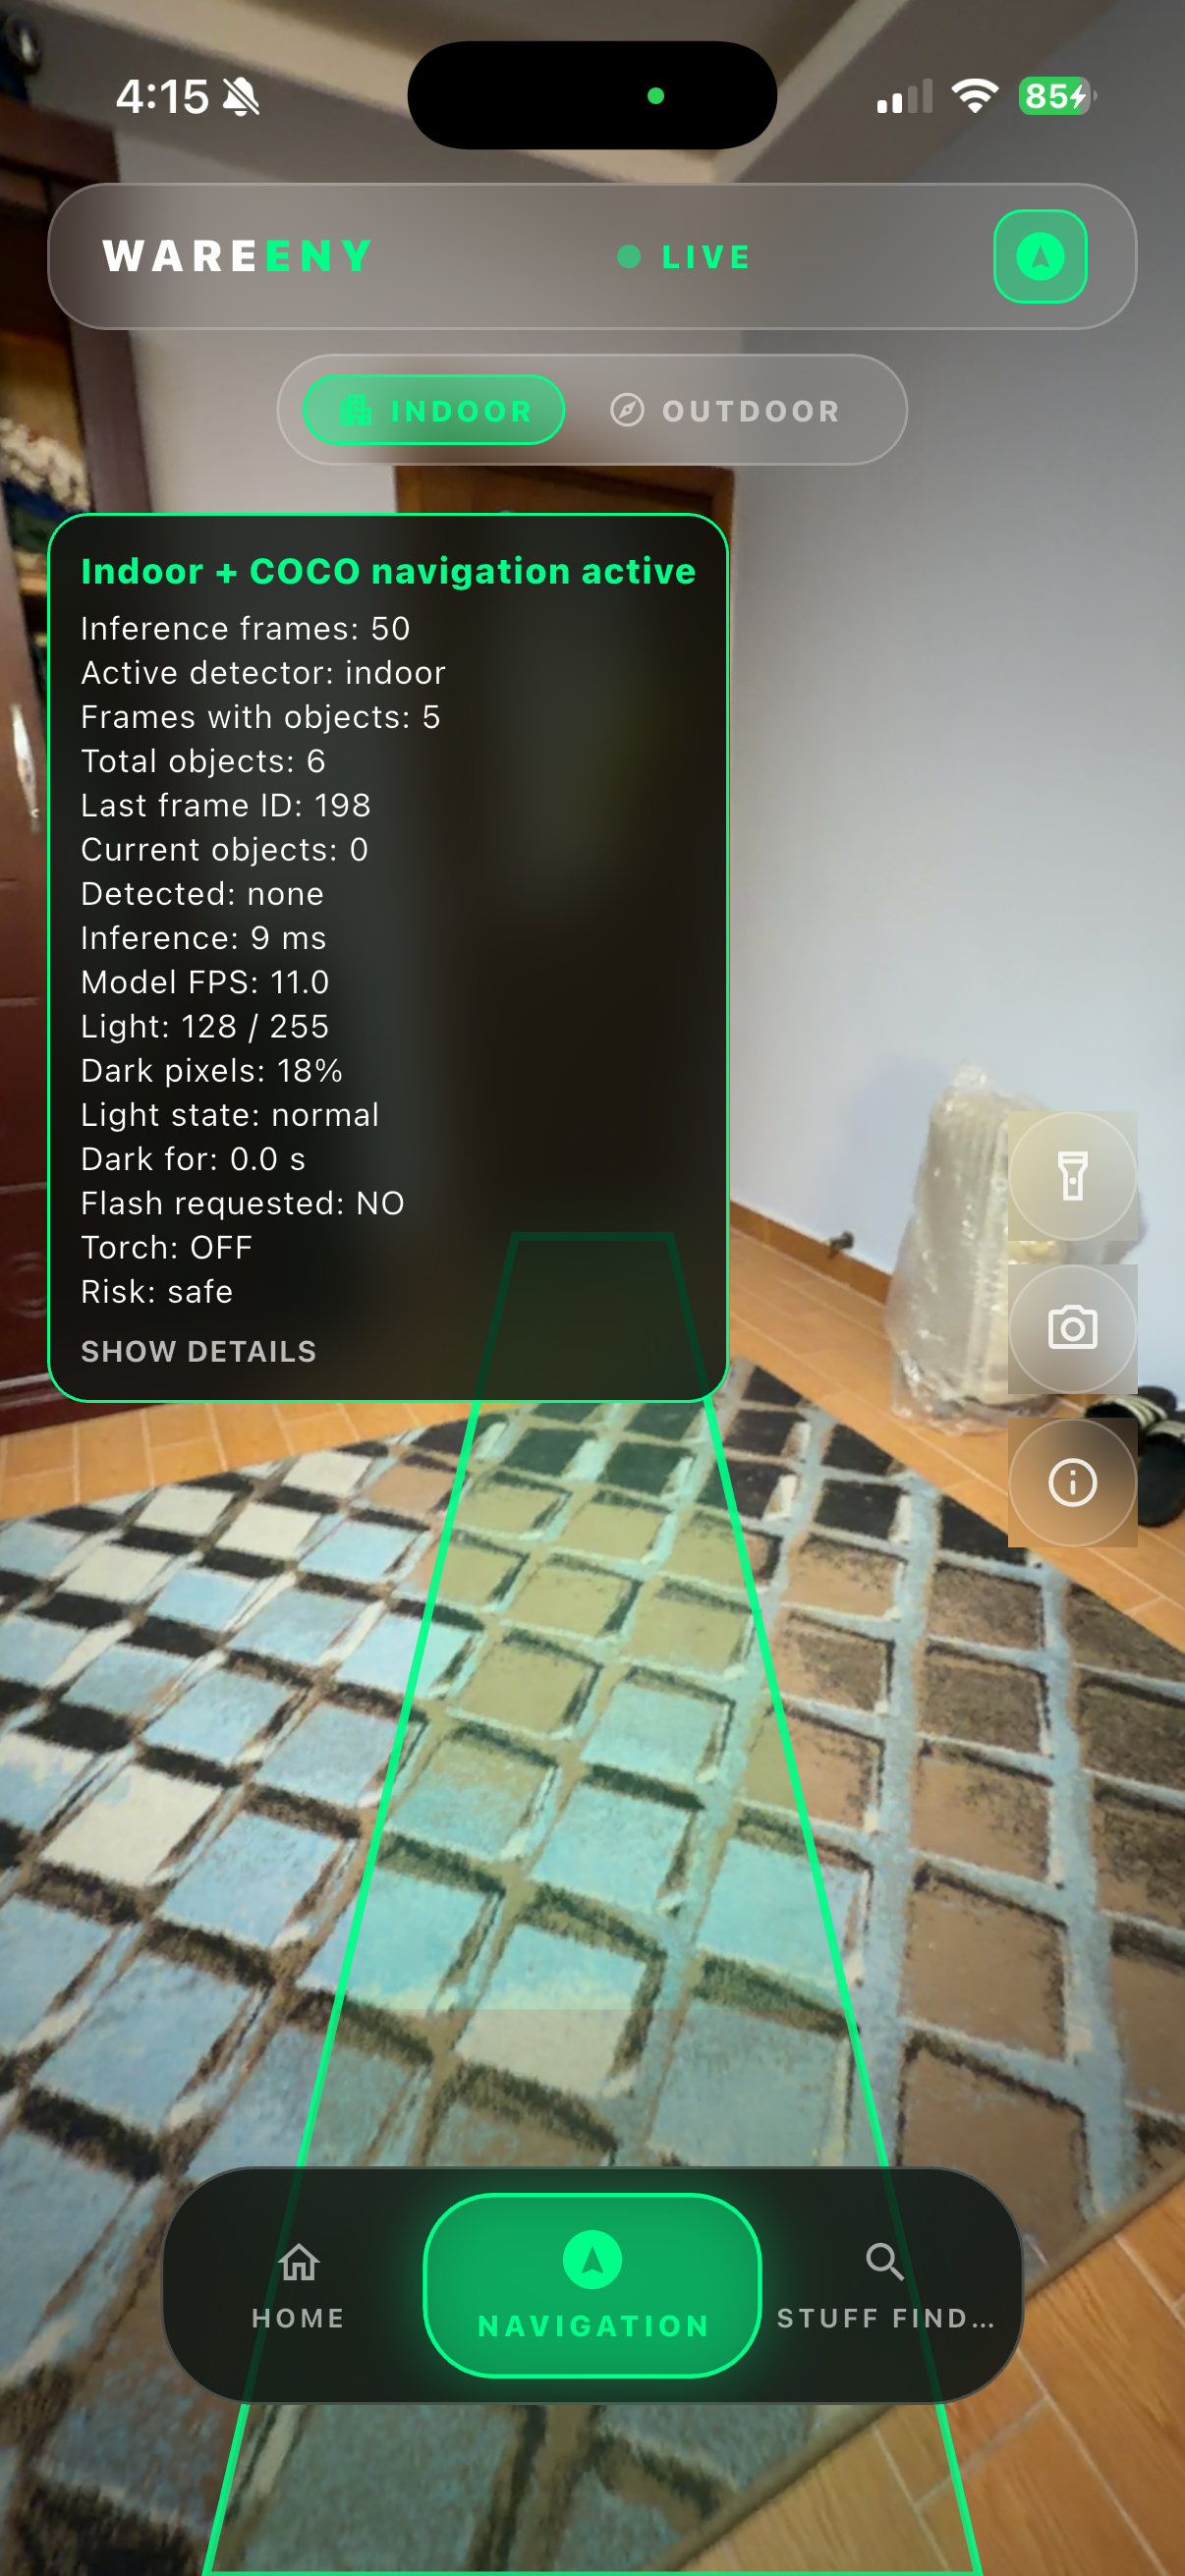
\includegraphics[width=0.32\textwidth]{figures/ui_navigation.png}
\caption{Navigation mode showing live detection overlays and directional status indicators.}
\label{fig:ui-navigation}
\end{figure}

\begin{figure}[ht]
\centering
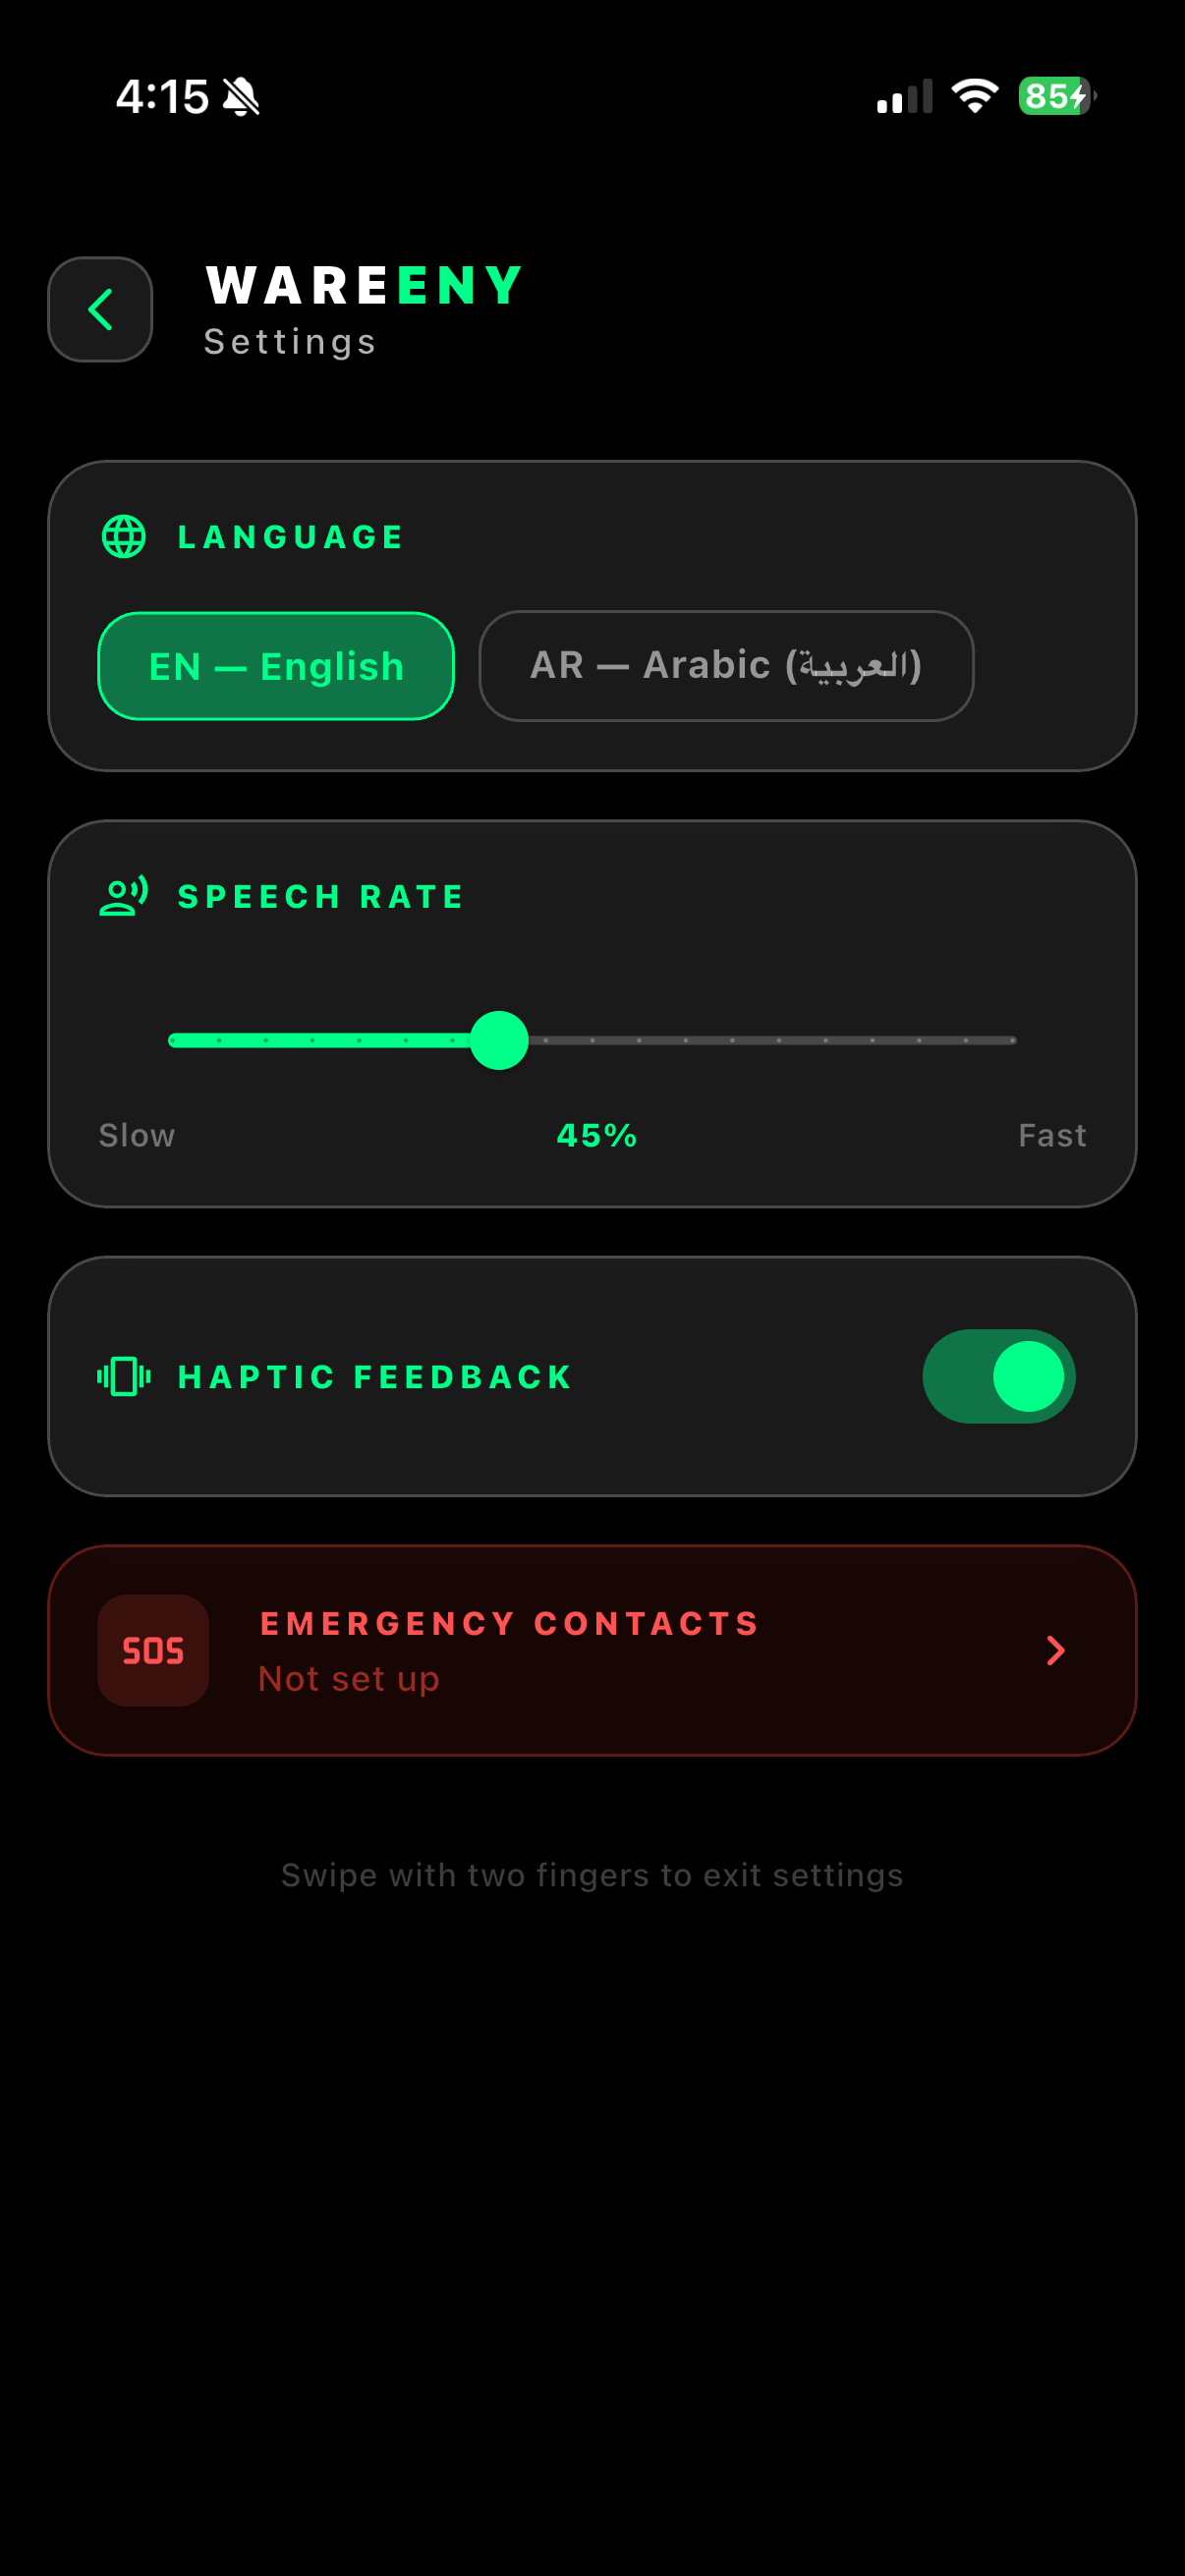
\includegraphics[width=0.32\textwidth]{figures/ui_settings.png}
\caption{Settings mode with language, speech-rate, and haptics configuration cards.}
\label{fig:ui-settings}
\end{figure}

\subsection{Bilingual Experience}
Wareeny supports English and Arabic at the application level. Locale changes propagate through \texttt{MaterialApp} and \texttt{AppLocalizations}, so labels, hints, and spoken announcements adapt to the selected language, and Flutter's bidirectional layout handling provides right-to-left presentation when Arabic is selected. Spoken output is matched to content: the navigation safety messages are issued in Egyptian Arabic, the money reader localizes the words around the amount while keeping the digits themselves, and the reading model answers in the language of the text it is reading.

\subsection{Feedback Strategy}
Feedback is intentionally multimodal. Visual overlays indicate live status, targets, and reading results; text-to-speech communicates prompts and findings; and categorized haptic signals support confirmation, navigation cues, obstacle warnings, and danger states. The audio layer incorporates completion and interruption handling so that feature controllers can manage reading state predictably---knowing, for example, when the queue has finished speaking. This combination makes the design more robust than dependence on any single output channel.

\subsection{Safety UI Overlay and Onboarding}
The interface integrates a dedicated safety layer consisting of the \texttt{EmergencyOnboardingScreen} and the modal \texttt{EmergencyOverlay}. The onboarding screen is shown on very first launch to explain the shake-to-activate mechanism using clear high-contrast buttons and spoken alerts, guiding the user to enter emergency contacts. The \texttt{EmergencyOverlay} is rendered with a dark translucent crimson gradient background showing a large pulsing red circular "SOS" button at the center. This design relies on standard animation parameters to communicate urgency visually while maintaining a full-screen gesture detector, allowing the user to abort the dispatch by tapping anywhere on the screen.

\section{Data Persistence}
\subsection{Persistence Philosophy}
Wareeny is a locally-operated assistive application. It does not maintain a user account, does not transmit personal data to any remote server, and does not log or store the results of any camera session. All data that the application persists across sessions fits into two conceptual categories: accessibility preferences that shape how the application behaves, and emergency contacts that the safety subsystem acts upon. Both categories are stored entirely on the device using Flutter's \texttt{SharedPreferences} key-value store, which provides zero-latency reads at startup and synchronous-style writes with no network dependency.

This choice is deliberate and appropriate to the domain. Visually impaired users depend on the application to respond instantly; any persistence mechanism that could introduce latency or failure---such as a remote database round-trip---would directly degrade the user experience. The stored data volume is also small: five scalar keys and one JSON-encoded list. A local SQL engine or cloud schema would add substantial complexity for no practical gain at the current scope of the project.

\subsection{Persisted Data Model}
The complete set of data persisted by the implemented application is summarized in Table~\ref{tab:prefs-schema}. Every entry is stored under a namespaced string key within \texttt{SharedPreferences} and is read once at application startup by \texttt{SettingsController}, which holds the values in memory for the duration of the session and writes them back immediately whenever the user makes a change.

\begin{table}[H]
\centering
\caption{Complete On-Device Persistence Model (\texttt{SharedPreferences})}
\label{tab:prefs-schema}
\begin{tabularx}{\textwidth}{|>{\raggedright\arraybackslash}p{0.38\textwidth}|>{\raggedright\arraybackslash}p{0.16\textwidth}|>{\raggedright\arraybackslash}X|}
\hline
\textbf{Key} & \textbf{Type} & \textbf{Purpose and Default} \\
\hline
\texttt{settings.locale} & String & Selected interface language (\texttt{`en'} or \texttt{`ar'}). Default: \texttt{`en'}. \\
\hline
\texttt{settings.speechRate} & Double & Text-to-speech output speed, clamped to a safe range. Default: \texttt{0.45}. \\
\hline
\texttt{settings.hapticsEnabled} & Boolean & Whether haptic vibration feedback is active. Default: \texttt{true}. \\
\hline
\texttt{settings.\allowbreak emergencyOnboardingSeen} & Boolean & Whether the first-launch emergency-contact onboarding screen has been shown. Default: \texttt{false}. \\
\hline
\texttt{settings.\allowbreak emergencyContacts} & String (JSON) & The list of trusted emergency contacts, serialized as a JSON array. Each element contains two fields: \texttt{name} (display label) and \texttt{phone} (international-format number). Default: empty list. \\
\hline
\end{tabularx}
\end{table}

\subsection{Emergency Contact Lifecycle}
The emergency contact list is the only structured data entity in the application. On first launch, the \texttt{EmergencyOnboardingScreen} prompts the user to add at least one trusted contact by entering a name and phone number. The contact is represented in code as an \texttt{EmergencyContact} value object with two fields---\texttt{name} and \texttt{phone}---and the full list is serialized to a single JSON string via \texttt{EmergencyContact.encodeList} before being written to \texttt{SharedPreferences}. On every subsequent launch the list is deserialized back into typed objects via \texttt{EmergencyContact.decodeList} and held in \texttt{SettingsController} memory.

The user may add, edit, or delete contacts at any time through \texttt{EmergencyContactsScreen}, which is accessible from the Settings mode. Every modification is immediately re-serialized and written back to storage, so the contact list is always current.

At the moment an emergency is triggered, the \texttt{EmergencyController} reads the in-memory contact list directly from \texttt{SettingsController}. It dials the first contact's phone number automatically, then iterates the full list to send an SMS message containing a Google Maps location link and to open a pre-filled WhatsApp message for each contact. No contact data is transmitted to any server; all communication channels are native device calls initiated on-device.

\subsection{Data That Is Not Persisted}
For completeness, Table~\ref{tab:not-persisted} documents the categories of data that are intentionally not stored, in order to clarify the system's privacy posture.

\begin{table}[H]
\centering
\caption{Data Categories Intentionally Not Persisted}
\label{tab:not-persisted}
\begin{tabularx}{\textwidth}{|>{\raggedright\arraybackslash}p{0.30\textwidth}|>{\raggedright\arraybackslash}X|}
\hline
\textbf{Category} & \textbf{Rationale} \\
\hline
Camera frames and captured images & Images are passed directly to the inference pipeline and discarded after the response is generated. No image file is retained on device or uploaded to any server. \\
\hline
Scan and read results & Spoken output is transient; results exist only in the \texttt{SpeechQueue} during playback and are not logged or saved. \\
\hline
Navigation and detection frames & Streaming detection frames are processed in memory and immediately discarded; no frame or detection record is written to storage. \\
\hline
GPS coordinates & Location is fetched on demand during an emergency dispatch, used to construct the SMS link, and then released. It is never stored. \\
\hline
\end{tabularx}
\end{table}

\chaptercover{5}{Chapter Five}{System Implementation and Testing}
\chapter{System Implementation and Testing}

\section{Introduction}
This chapter explains how the Wareeny design has been translated into working application modules. The implementation is mode-oriented and controller-driven: rather than building every assistive feature at once, the repository organizes the work into reusable services that support multiple assistive tasks over time. The result is a build that contains both fully usable user flows and clearly marked extensibility points for features that are planned but not yet surfaced as finished screens.

\subsection{Implementation Approach}
The approach is incremental. Shared application concerns---environment configuration, dependency registration, audio output, localization, and persistence---are established first, and feature controllers are then layered on top so that each mode owns its logic without duplicating infrastructure. This is visible in the separation between shared services such as \texttt{VlmAssistant} and \texttt{ObjectDetectionSource} and feature-specific controllers such as \texttt{VlmReadController}, \texttt{NavigationController}, and \texttt{StuffFinderController}. A single design rule underpins the AI work: screens and controllers talk only to the \texttt{VlmAssistant}, never to a provider directly, which keeps routing and fallback policy in one place.

\section{System Tools}
Table~\ref{tab:system-tools} lists the principal tools and packages used in the implementation, with the versions resolved in the project's \texttt{pubspec.lock}.

\begin{table}[ht]
\centering
\caption{Implementation Tools and Versions}
\label{tab:system-tools}
\begin{tabularx}{\textwidth}{|>{\raggedright\arraybackslash}p{0.34\textwidth}|>{\raggedright\arraybackslash}p{0.15\textwidth}|>{\raggedright\arraybackslash}X|}
\hline
\textbf{Tool / Package} & \textbf{Version} & \textbf{Role} \\
\hline
Flutter SDK & 3.x (stable) & Cross-platform UI framework \\
\hline
Dart SDK & $\geq$ 3.12.0 & Application language \\
\hline
\texttt{camera} & 0.12.0+1 & Still-image capture for Scan and Read \\
\hline
\texttt{ultralytics\_yolo} & 0.6.2 & Streaming YOLOv8n detection \\
\hline
\texttt{flutter\_tts} & 4.0.2 & Bilingual text-to-speech output \\
\hline
\texttt{shared\_preferences} & 2.2.0 & Local key-value persistence \\
\hline
\texttt{sensors\_plus} & 6.1.0 & Accelerometer (shake detection) \\
\hline
\texttt{geolocator} & 13.0.2 & GPS location for emergency dispatch \\
\hline
\texttt{flutter\_phone\_direct\_caller} & 2.0.1 & Native auto-dialing \\
\hline
\texttt{url\_launcher} & 6.3.1 & SMS / WhatsApp / maps intents \\
\hline
\texttt{permission\_handler} & 11.4.0 & Runtime permissions \\
\hline
\texttt{image} & 4.3.0 & Off-isolate image downscale/re-encode \\
\hline
YOLOv8n (nano, INT8) & Ultralytics & Bundled detection model for navigation and object finding \\
\hline
Gemma 4 (self-hosted) & Google DeepMind & Vision-language model served by the cloud VLM backend \\
\hline
\end{tabularx}
\end{table}

\subsection{Frontend and UI Tooling}
Flutter is the main frontend framework, with \texttt{MaterialApp}, animated widgets, semantics, localization delegates, and custom reusable components used throughout. Reactive updates use the standard \texttt{ChangeNotifier}/\texttt{AnimatedBuilder} pattern, so controllers expose plain observable state and screens rebuild from it. The \texttt{camera} package supplies still-image capture for Read and Scan.

\subsection{AI and Model Tooling}
The repository integrates two AI tool paths. For reading, scanning, and future reasoning tasks, a vision-language layer is implemented through the local and cloud provider abstractions, routed by \texttt{ModelRouter} and coordinated by \texttt{VlmAssistant}; the cloud tier targets a self-hosted Gemma 4 model over HTTP with Server-Sent Events. For real-time navigation and object finding, the \texttt{ultralytics\_yolo} package runs bundled YOLOv8n (nano, INT8) assets on a live stream. The \texttt{image} package is used inside the cloud provider to decode, downscale, and re-encode captures before transmission, which reduces upload and inference overhead and is run off the UI isolate to avoid jank.

\subsection{Platform Services and Assets}
Audio output is implemented through \texttt{flutter\_tts} inside the \texttt{AudioHapticsBridge}, with language-aware voice selection and categorized haptics. \texttt{SharedPreferences} provides lightweight settings storage. Model assets are bundled under \texttt{assets/models} and include the general YOLOv8n navigation detector and the custom stuff-finder detector, each shipped in Android (TFLite, INT8) and iOS (Core ML) formats; a dedicated Egyptian-pound banknote detector is reserved for future work. Environment-dependent backend and model identifiers are resolved through \texttt{AppConfig}, which distinguishes development and production configurations and reads overrides from compile-time environment values.

\section{Core Features Implemented}
Because Wareeny is an assistive mobile application rather than a transaction-oriented information system, its implemented core features are best described as functional modes and service flows rather than database operations. The only persisted data operations are the reading and updating of user settings through \texttt{SharedPreferences}. The major implemented features are summarized below.

\subsection{Mode-Based Navigation Shell}
\texttt{NavigationShell} is the top-level interaction hub. It speaks a greeting on first launch, exposes the application modes through a reusable carousel, and supports two-finger swipe switching. The shell hosts dedicated branches for Settings, Read, Scan, Navigation, and Stuff Finder, with Home serving as the camera-centred entry surface. This gives the application a stable assistive framework while individual features continue to evolve.

\subsection{Scan Mode with Hybrid VLM Routing}
Scan is implemented through \texttt{ScanScreen} and the shared \texttt{VlmReadController}. A single tap captures a high-resolution still and submits a scan task, and the \texttt{ModelRouter} attempts the on-device vision-language model first and the self-hosted backend second. The model handles the subject as a product read off its label, a sign or document reduced to its key facts, a banknote whose denomination is reported, or a plain object. Currency is exposed as a distinct task in the routing policy so that a specialized on-device banknote provider---a custom YOLOv8n model trained on both faces of the six circulating Egyptian-pound denominations (5, 10, 20, 50, 100, and 200)---can later be registered ahead of the language model for accurate, fully offline denomination reading. That dedicated detector and its accuracy evaluation are reserved for future work; in the current build, denomination reading is served by the vision-language pipeline like every other scan subject. This design deliberately isolates the one task where a general vision-language model is weakest behind a provider boundary, so the specialized detector can be added later without disturbing the screens or controllers that depend on it.

\subsection{Read Mode with Hybrid VLM Routing}
Read mode is implemented through \texttt{ReadScreen} and \texttt{VlmReadController}. The user captures a still and the controller submits a read task through \texttt{VlmAssistant}; \texttt{ModelRouter} prefers the on-device model and falls back to the self-hosted backend when the local runtime is unavailable. Streamed token deltas are collected into sentence-sized chunks using sentence-terminator boundaries (including Arabic punctuation) and spoken through \texttt{SpeechQueue}, while the interface keeps stop, repeat, skip, and cancel controls available until both generation and playback have finished. A tuned prompt keeps the output a faithful reading of the main body rather than a summary.

\subsection{Real-Time Navigation Mode}
Navigation mode is implemented through \texttt{NavigationScreen}, \texttt{NavigationController}, and \texttt{NavigationRiskEngine}. A YOLO streaming view produces detection frames, which are oriented and passed into a geometric risk model. The controller filters unstable detections through confirmation windows and cooldown rules before generating spoken messages or haptic alerts, and it can announce left-side avoidance, right-side avoidance, a frontal stop condition, a low-light warning, or a path-clear state after enough consecutive safe frames. Indoor and outdoor submodes are available in the interface and currently share the same pipeline, preparing the system for later environment-specific tuning.

\subsection{Stuff Finder Mode}
Stuff Finder is implemented through \texttt{StuffFinderScreen} and \texttt{StuffFinderController}. The user selects a target from a curated list combining common COCO classes with custom assistive targets such as wallet, glasses, and keys. After selection the detector is started, the appropriate model path is chosen, and streaming frames are filtered so that only detections matching the selected label reach the feature logic. The controller announces the chosen target, reports matches through speech, and suppresses repetitive announcements with a cooldown.

\subsection{Settings, Localization, and Personalization}
Settings are implemented through \texttt{SettingsScreen} and \texttt{SettingsController}. The user can switch between English and Arabic, adjust the speech rate within a clamped range, and toggle haptics. Each value is persisted immediately and reflected across the application through reactive rebuilds. This matters because Wareeny is not only an inference tool but a personalized assistive interface whose output behaviour must adapt to the user's preferred language and feedback style.

\subsection{Audio and Haptic Delivery}
Audio and haptic behaviour is handled centrally so that every feature shares one feedback layer. The \texttt{AudioHapticsBridge} initializes speech early, prefers an Egyptian-Arabic voice when one is installed, applies speech-rate updates, and exposes completion and cancellation callbacks; haptics are exposed through semantic categories such as danger, obstacle, navigation cue, and confirmation. This shared layer simplifies controller design, because feature modules never manage raw text-to-speech configuration themselves.

\subsection{Safety and Emergency Dispatch (CRUD on Emergency Contacts)}
The safety and emergency subsystem is designed for low-latency activation during critical events. Trusted emergency contacts are managed locally by the user. The application supports full CRUD operations (Create, Read, Update, Delete) on emergency contact details (name and phone number) via the \texttt{EmergencyContactsScreen}. This is stored and serialized as a JSON string under the \texttt{settings.emergencyContacts} key.

The execution logic utilizes the device accelerometer: the \texttt{ShakeDetectorService} monitors physical acceleration. When a shake signature is identified, the \texttt{EmergencyController} starts a 5-second cancelable countdown timer. The user is notified via audio ("5, 4, 3, 2, 1") and pulsing haptics. If the timer is not aborted, the controller fetches GPS coordinates using the \texttt{LocationService}, dials the primary contact natively, silently transmits a text message with the Google Maps coordinates (using a custom Android SMS method channel or fallback SMS URL), and pre-fills a redundant WhatsApp message.

\section{User Interface Organized and Documented}
\subsection{Reusable Widgets}
The interface is organized around reusable widgets rather than monolithic screens---examples include \texttt{CameraTopBar}, \texttt{ModeCarouselBar}, \texttt{CameraSideActions}, the reading-status pill, the scan-result view, and mode-specific overlays. Each widget has a clearly bounded responsibility, which improves maintainability and keeps styling consistent across modes.

\subsection{Screen Composition and Overlays}
Each major feature screen is built as a stack over a full-screen camera layer or a settings surface, with overlays placed for branding, status, target selection, reading state, optional diagnostics, and mode switching. This layered composition suits assistive camera applications: it preserves a stable visual hierarchy while allowing live perception information to appear without replacing the underlying preview.

\subsection{Accessibility Semantics}
Accessibility semantics are integrated directly into the interface. Mode switching exposes custom semantics actions, important status values are marked as live regions, target selectors and controls are labelled for screen-reader use, and announcements are spoken when major mode changes occur. The semantics model is therefore part of the user-interface implementation itself, not a documentation afterthought.

\subsection{Documented Screens}
Figures~\ref{fig:impl-scan}--\ref{fig:impl-stufffinder} document the implemented screens captured from the running application.

\begin{figure}[ht]
\centering
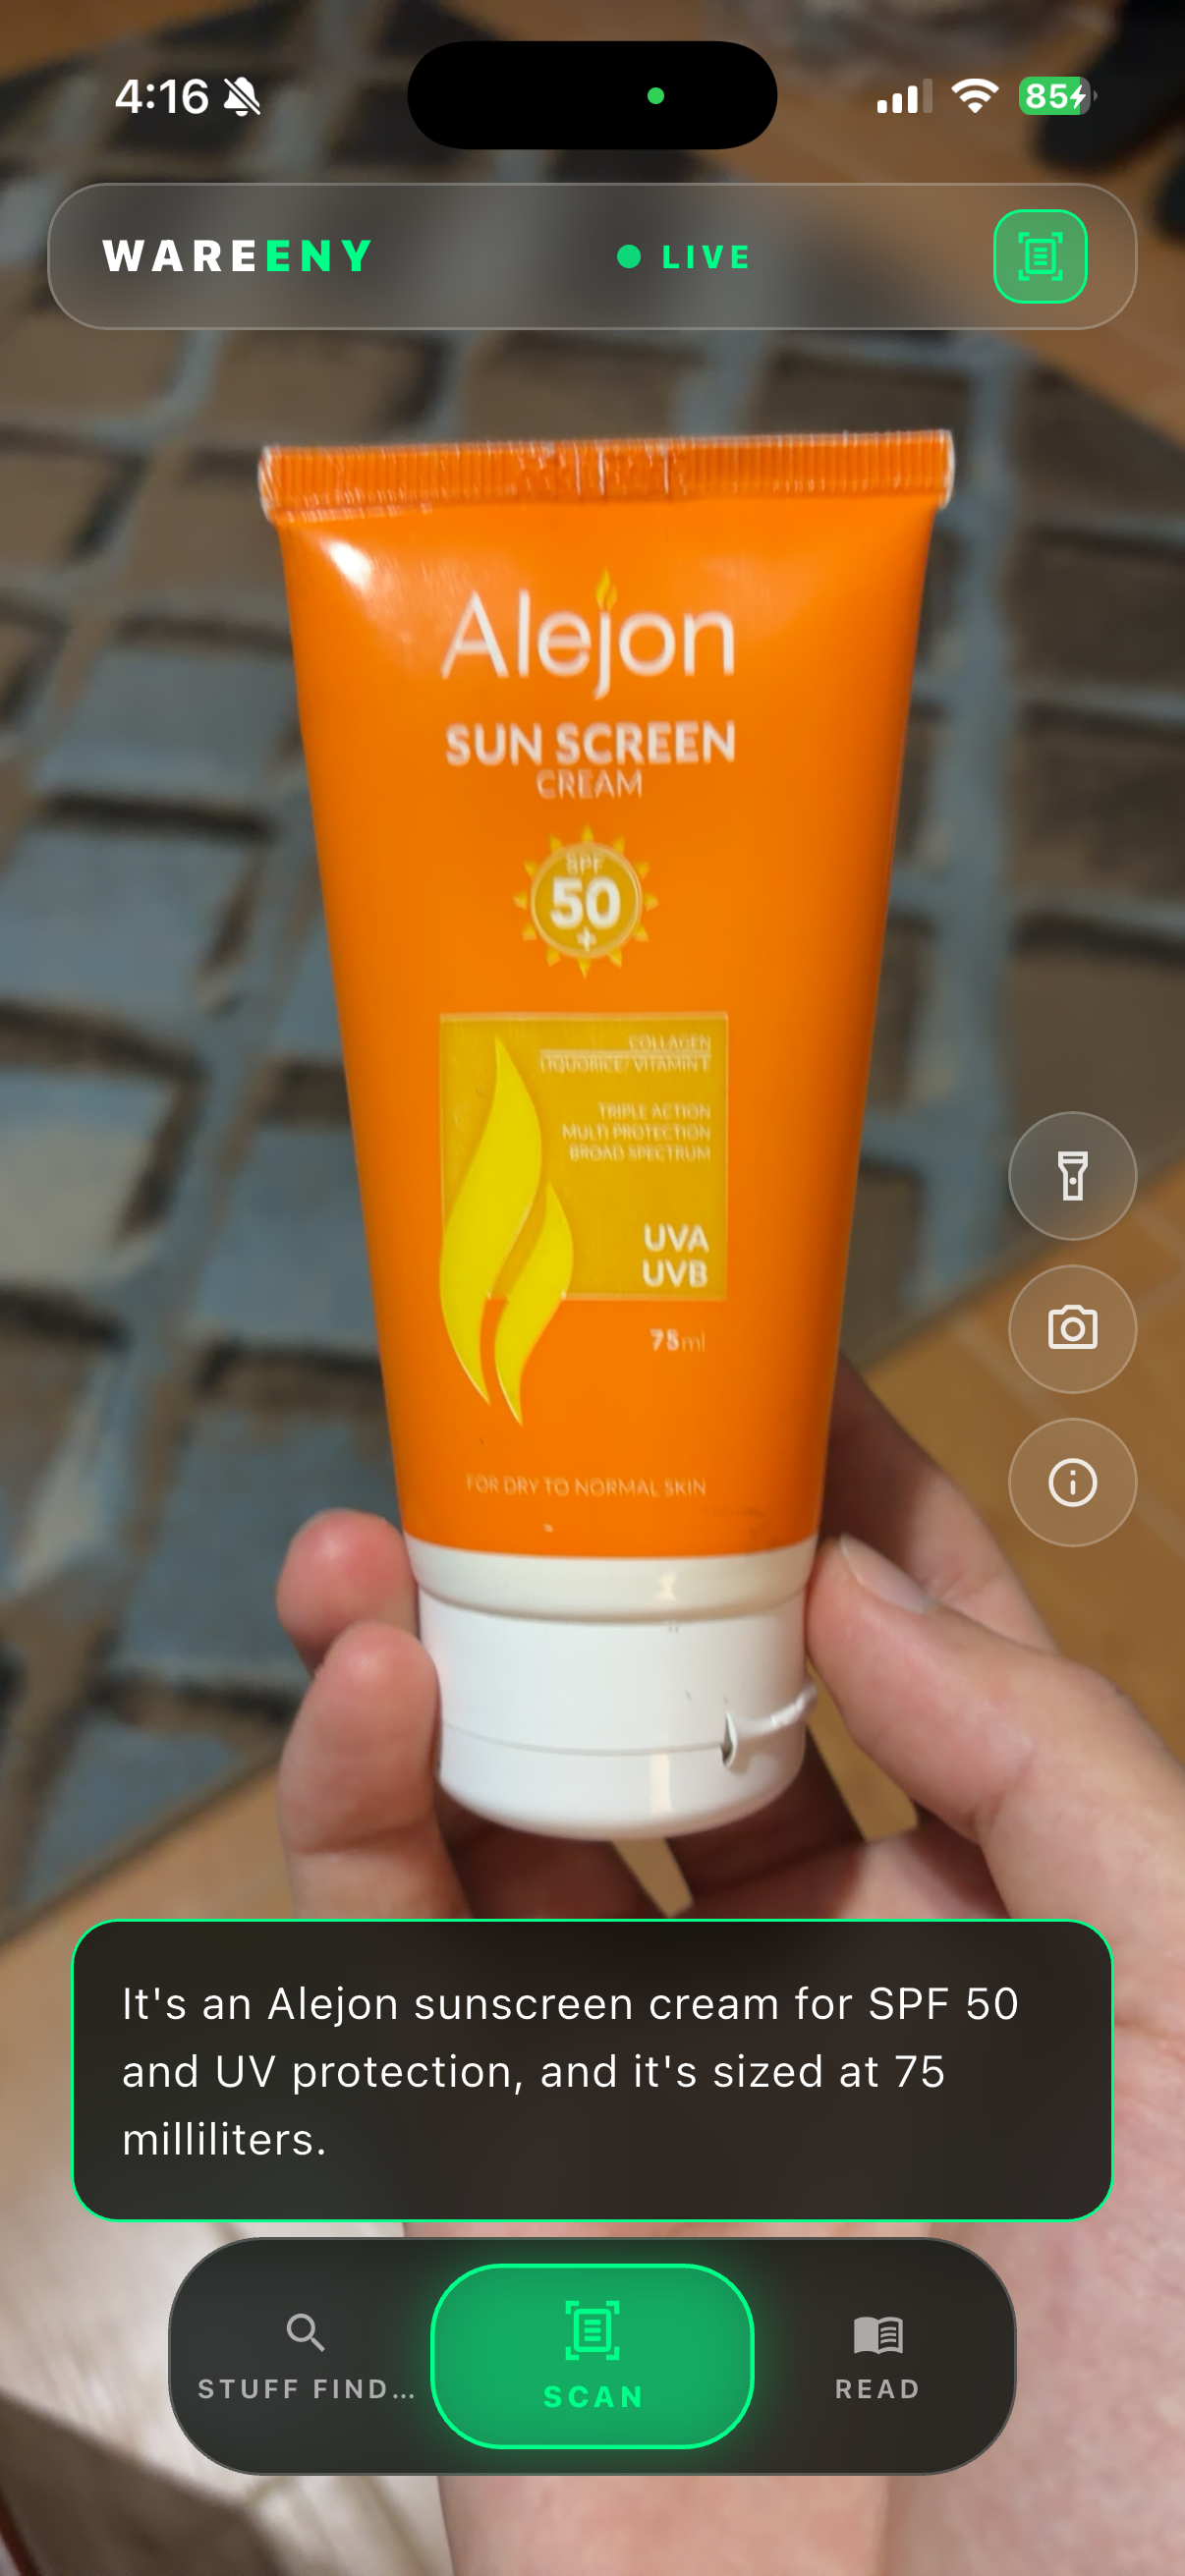
\includegraphics[width=0.32\textwidth]{figures/impl_scan.png}
\caption{Scan mode after a capture, showing the spoken-result overlay and repeat action.}
\label{fig:impl-scan}
\end{figure}

\begin{figure}[ht]
\centering
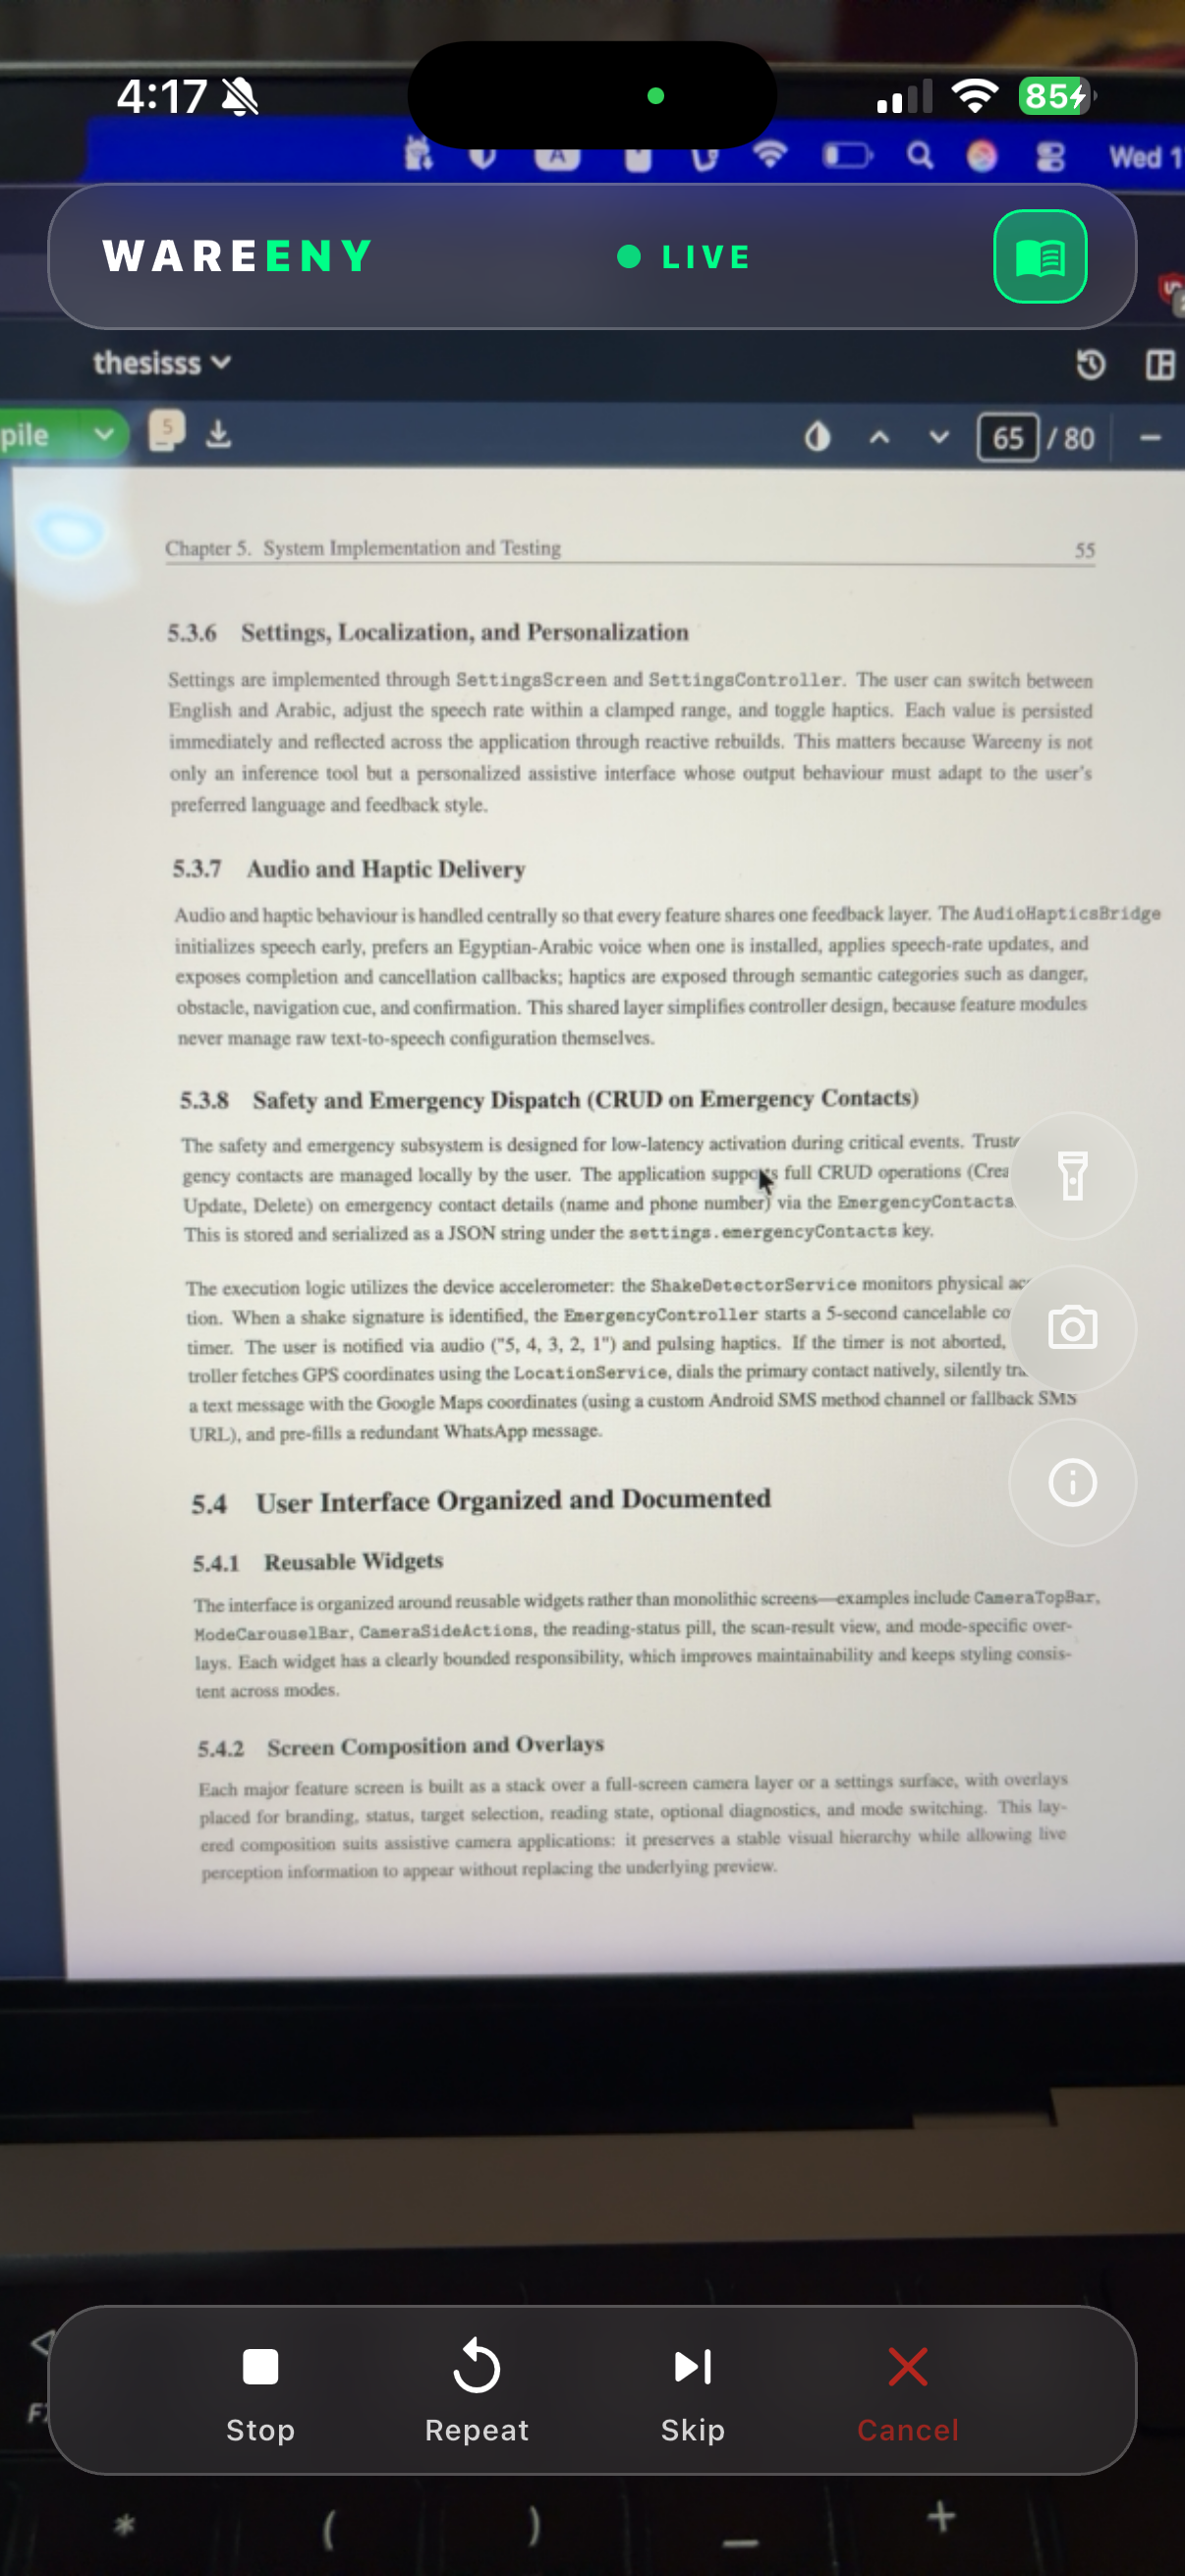
\includegraphics[width=0.32\textwidth]{figures/impl_read.png}
\caption{Read mode with stop, repeat, skip, and cancel controls during progressive speech.}
\label{fig:impl-read}
\end{figure}

\begin{figure}[ht]
\centering
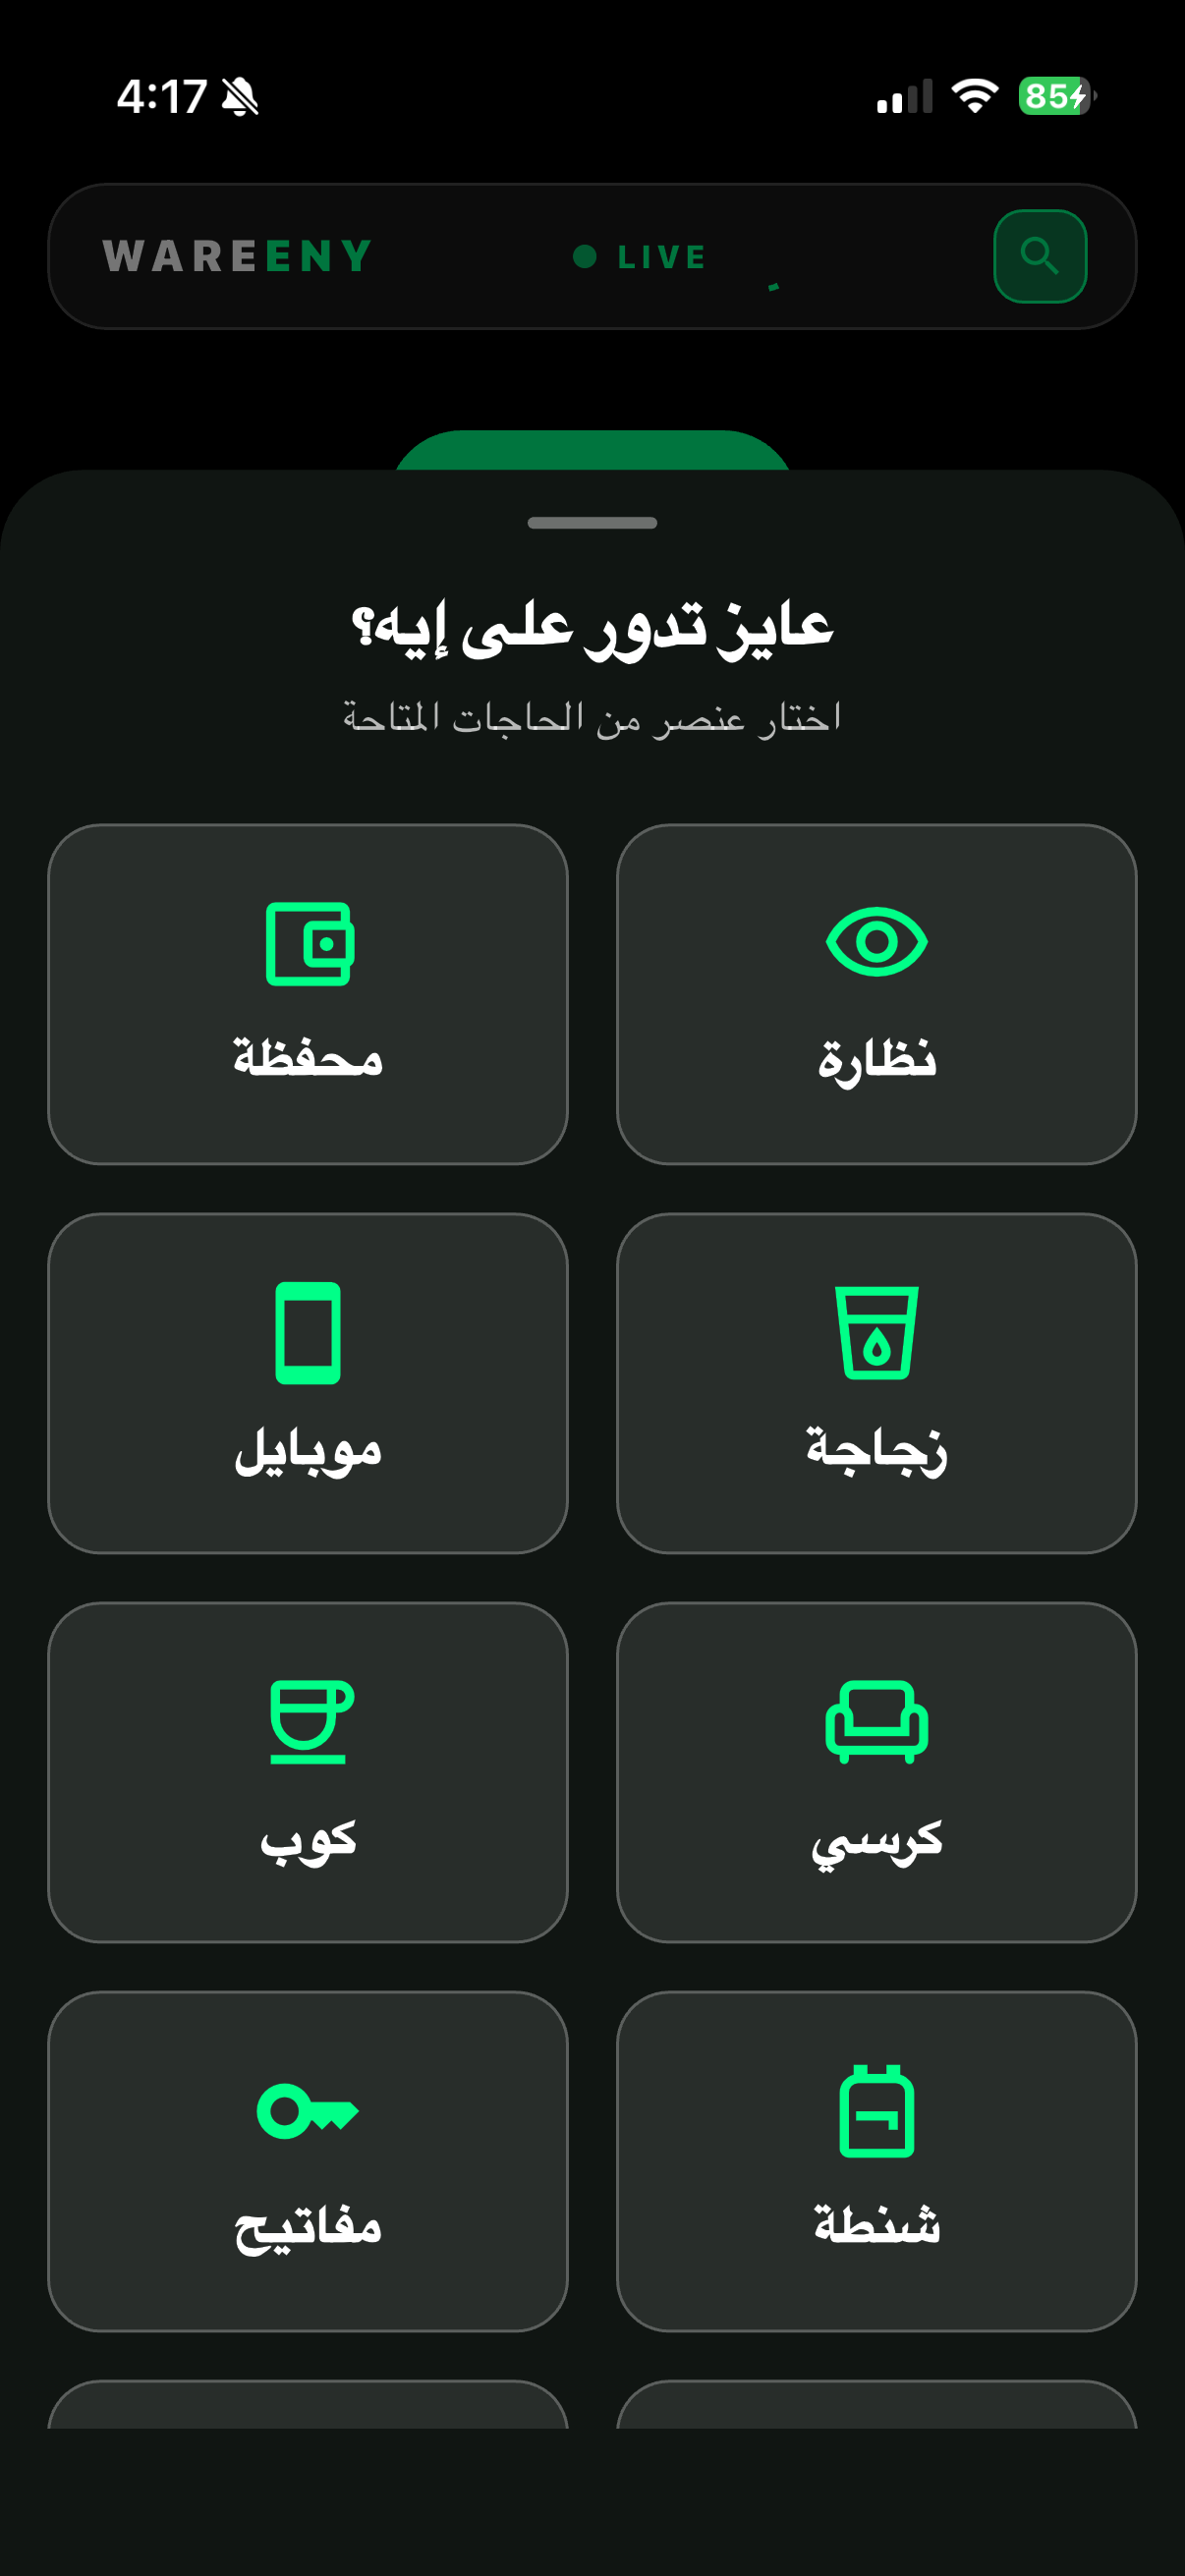
\includegraphics[width=0.32\textwidth]{figures/impl_stufffinder.png}
\caption{Stuff Finder target picker merging custom assistive classes with COCO classes.}
\label{fig:impl-stufffinder}
\end{figure}

\section{Source Code Organized and Documented}
\subsection{Bootstrap and Dependency Injection}
Application startup is centralized in \texttt{bootstrap}, which initializes the widget binding, loads configuration, restores settings, builds the service registry, and eagerly prepares audio. \texttt{ServiceRegistry} is the single place where the settings controller, the bridges, the three vision-language providers, the model router, the assistant, and the detection source are wired together; the assembled services are then exposed to the widget tree through \texttt{AppScope}. Concentrating construction here keeps cross-cutting dependencies out of feature screens.

\subsection{Feature Controllers}
Feature behaviour lives in controllers rather than view code. \texttt{VlmReadController} manages the capture-to-speech state machine for both Scan and Read, \texttt{NavigationController} manages streaming analysis and feedback timing, \texttt{StuffFinderController} manages target-based detection and announcements, and \texttt{SettingsController} manages persistent preferences. This separation improves readability, testability, and maintainability by keeping business logic out of widget rendering.

\subsection{Shared AI and Detection Services}
Shared services---\texttt{VlmAssistant}, \texttt{ModelRouter}, \texttt{VlmPrompts}, the local, cloud, and currency providers, \texttt{ObjectDetectionSource}, \texttt{BanknoteDetector}, and \texttt{NavigationRiskEngine}---serve as reusable infrastructure, letting multiple modes share the same inference foundations without coupling controllers to backend details or model implementations. This matters in assistive software, where new features typically extend existing perception capabilities rather than starting from scratch.

\subsection{Emergency Subsystem Classes}
The emergency subsystem resides under \texttt{lib/core/emergency/} and is composed of:
\begin{itemize}
  \item \texttt{EmergencyController}: Coordinates the overall state machine, countdown triggers, and Native SMS/dialer routing.
  \item \texttt{ShakeDetectorService}: Listens to the accelerometer stream from \texttt{sensors\_plus} and filters qualifying user-shake events.
  \item \texttt{LocationService}: Integrates with the native location APIs via \texttt{geolocator} to retrieve current latitude and longitude.
  \item \texttt{EmergencyContact}: Defines the data entity and provides JSON serialization logic for persistence.
\end{itemize}

\subsection{Representative Source Listings}
Two short listings illustrate the design rules described above. Listing~\ref{lst:router} shows the \texttt{ModelRouter} policy: a pure, side-effect-free function that returns the provider order for each task, keeping all routing decisions in one place. Listing~\ref{lst:emergency} shows the emergency dispatch sequence, which fetches location and dials in parallel before sending SMS and WhatsApp messages to each contact.

\begin{lstlisting}[language=Java,caption={Task-aware provider routing policy (\texttt{model\_router.dart}).},label=lst:router]
/// Providers to attempt for [task], in order of preference.
List<VlmProvider> providersFor(VlmTask task) => switch (task) {
      VlmTask.scan ||
      VlmTask.read ||
      VlmTask.inHand ||
      VlmTask.currency ||
      VlmTask.brand =>
        [_local, _cloud],
      VlmTask.askImage || VlmTask.describeScene => [_cloud, _local],
    };
\end{lstlisting}

\begin{lstlisting}[language=Java,caption={Emergency dispatch sequence (\texttt{emergency\_controller.dart}).},label=lst:emergency]
Future<void> _triggerEmergency() async {
  onEmergencyTriggered?.call();

  final contacts = settings.emergencyContacts;
  final dialNumber =
      contacts.isNotEmpty ? contacts.first.phone : _fallbackEmergencyNumber;

  // Fetch GPS + auto-dial simultaneously for speed.
  final locationFuture = locationService.getCurrentPosition();
  await _autoCall(dialNumber);

  final position = await locationFuture;
  final mapsLink =
      position != null ? locationService.toGoogleMapsLink(position) : null;

  // Send SMS silently (Android: SmsManager; iOS: falls back to sms: URI).
  for (final contact in contacts) {
    await _sendSmsAuto(contact, mapsLink);
  }
  // Open WhatsApp with a pre-filled message for each contact.
  for (final contact in contacts) {
    await _openWhatsApp(contact, mapsLink);
  }
}
\end{lstlisting}

\section{Test Plan and Test Cases}
\subsection{Functional Test Cases}
\begin{itemize}
  \item TC-01: Verify that startup restores the persisted language, speech-rate, and haptics preferences and presents the navigation shell correctly.
  \item TC-02: Verify two-finger gesture mode switching and the correct semantic announcement of the newly active mode.
  \item TC-03: Verify Scan behaviour from still capture through routed response to spoken completion, including the ``repeat result'' gesture.
  \item TC-04: Verify Scan money reading: a single Egyptian-pound note is spoken as its denomination, and multiple notes are spoken as a correct total plus breakdown.
  \item TC-05: Verify Read behaviour, including token streaming and the stop, repeat, skip, and cancel controls.
  \item TC-06: Verify navigation warning generation for left, right, frontal-danger, low-light, and path-clear conditions.
  \item TC-07: Verify Stuff Finder target selection, detector startup, match filtering, and cooldown-gated speech.
  \item TC-13: Verify that shaking the device initiates the 5-second countdown timer and announces countdown values.
  \item TC-14: Verify that tapping the screen during the countdown aborts the emergency dispatch and announces cancellation.
  \item TC-15: Verify that completing the countdown triggers location fetch, dials the primary contact, sends silent SMS (Android), and opens pre-filled WhatsApp.
\end{itemize}

\subsection{Integration and Fallback Cases}
\begin{itemize}
  \item TC-08: Verify that a non-money frame causes the banknote detector to report unavailable and the request to fall through to the vision-language tier.
  \item TC-09: Verify on-device-provider unavailability and correct backend fallback for reading.
  \item TC-10: Verify the unavailable-state message when neither the on-device nor the backend tier can serve a request.
  \item TC-11: Verify model-path switching between the general navigation asset and the custom stuff-finder asset.
  \item TC-12: Verify settings and emergency contacts list persistence across application restarts.
\end{itemize}

\subsection{Automated Test Coverage}
Unlike a purely manual specification, the repository ships an executable unit-test suite that exercises the deterministic core of each subsystem in isolation from the camera, network, and native runtime. It covers the navigation risk engine's geometric assessment, the detection coordinate mapper's rotation and mirroring logic, the YOLO detection source's frame parsing, the stuff-finder controller and screen behaviour, the navigation controller's confirmation and cooldown timing (driven by an injected clock), and the banknote announcement function's total-and-breakdown formatting in both languages. Because these components were written with injectable dependencies and pure functions where possible, they are testable without device hardware. The flows that genuinely depend on camera input, platform views, speech, haptics, model assets, and backend availability remain verified through functional, device-based testing; the overall plan is therefore strongest as a combination of automated unit tests for core logic and integration testing for end-to-end behaviour.

\section{Testing the Core Features with Sample Data}
\noindent The implemented features were exercised with representative samples chosen to mirror the intended user tasks. Instead of describing only the testing procedure, this section records the sample type, the representative output produced by the feature, and the practical meaning of that output. In total, the sample suite covered reading/scanning cases across signs, labels, documents, objects, and currency; navigation cases across five live-scene conditions; stuff-finder cases across both custom assistive targets and common object classes; settings persistence across the three stored preferences; and emergency behaviour across trigger, cancel, and full-dispatch scenarios.

\subsection{Reading and Scanning Samples}
Reading and scanning were tested with six representative sample types: a printed sign, a short packaged-product label, a multi-line notice, a document paragraph, a single Egyptian-pound note, and a mixed-note money sample. In scan-oriented cases, the intended behaviour was a short, direct spoken result rather than a raw OCR dump. For example, a sign sample reading ``Emergency Exit'' was expected to produce a concise spoken output such as ``Emergency exit''; a product label was expected to return the product identity or key fact rather than every visible character; a single-note money sample was expected to produce the denomination directly (for example, ``20 Egyptian pounds''); and a mixed-note sample was expected to produce a total plus breakdown (for example, ``Total 70 pounds: 50 and 20''). In read-oriented cases, the output was expected to remain longer and closer to the body text, with playback controls staying available until the spoken queue had drained.

These reading and scanning outputs are stronger than those of a purely classical OCR-style path in two ways. First, the result is shaped by user intent: scan returns a concise answer, while read returns a fuller spoken rendering. Second, the output is semantically useful rather than a flat transcription. Quantitatively, this design direction is consistent with the literature cited earlier: interactive/contextual visual assistance outperformed static captioning by 40\% in task completion [1], and specialized Arabic-reading pipelines improved from 68\% to 89\% on difficult Arabic text, a gain of 21 percentage points over the generic baseline [2].

\subsection{Navigation Samples}
Navigation was tested with five live-scene conditions: a clear corridor, a centrally placed obstacle, a left-offset obstacle, a right-offset obstacle, and a low-light environment. The representative outputs for these scenes were respectively a path-clear announcement, a frontal-danger or stop warning, a directional avoidance cue instructing movement away from the left-side object, a directional avoidance cue for the right-side object, and a low-light warning. Because these cases are streamed rather than single-shot, they also verified the confirmation-window logic and the cooldown behaviour that suppresses repetitive warnings.

The result of these cases is not simply that the detector recognizes objects, but that it converts detections into actionable mobility feedback. This is the area where the classical detector path remains the correct choice for the thesis system: published assistive-detection results place comparable YOLO-style pipelines in the 12.8--15.2 FPS range on mobile hardware [4], [5], making them suitable for real-time safety guidance.

\subsection{Stuff-Finder Samples}
Stuff Finder was tested with six representative targets: keys, glasses, wallet, bottle, chair, and cell phone. These samples intentionally cover both custom assistive targets and common object classes. The representative output sequence for a successful test was: target-selection confirmation (for example, ``Searching for keys''), live filtering of frames to the chosen class only, and a match announcement such as ``Found keys'' when the target entered view. Repeated sightings were expected not to trigger repeated speech immediately, because the cooldown layer must suppress redundant announcements.

This feature improves over a generic detector-view workflow because the user does not receive every detected label in the frame. Instead, the system narrows the spoken output to a single user-chosen target, which reduces cognitive load and makes the detector practically usable as a retrieval aid rather than as a passive recognition demo.

\subsection{Settings Persistence Samples}
Settings persistence was tested across the three stored preferences: language, speech rate, and haptics. A representative validation sequence changed the interface language from English to Arabic, adjusted the speech rate, disabled or re-enabled haptics, and then restarted the application. The successful output of this test was not a spoken caption but state restoration: the application reopened with the same locale, the same speech-rate behaviour, and the same haptics setting already applied. This confirms that the implemented persistence layer correctly retains the user-personalization values that matter most to daily use.

\subsection{Emergency Dispatch Verification}
The emergency subsystem was verified through three representative scenarios: trigger, cancel, and full dispatch. In the trigger scenario, a shake gesture produced the countdown overlay and the spoken sequence ``5, 4, 3, 2, 1'' with synchronized haptics. In the cancel scenario, tapping during the countdown terminated the process and returned the interface to a safe idle state. In the full-dispatch scenario, completing the countdown caused the controller to fetch location data, open the dialer for the primary contact, and prepare a text message containing a Google Maps link built from the captured latitude and longitude.

From a thesis perspective, the value of this feature is not accuracy in the image-recognition sense but reliability of safety flow. The tested outputs confirm that the emergency path progresses through all three required states---armed warning, user-cancel opportunity, and full dispatch---without requiring visual interaction.

\subsection{Testing Summary and Interpretation}
The testing evidence combines representative scenario validation with automated unit coverage rather than relying solely on abstract specification. This chapter therefore reports concrete sample inputs, representative outputs, and scenario coverage instead of presenting unmeasured repository-wide accuracy percentages. Where quantitative superiority is discussed, it is anchored in the cited literature that motivated the adopted architecture: a 21 percentage-point improvement from 68\% to 89\% for specialized Arabic reading over a generic OCR baseline [2], a rise from 72\% to 94\% in controlled Egyptian-currency recognition for localized models over generalized transfer learning [3], and a 40\% task-completion improvement for interactive VQA-style assistance over static captioning [1]. The Wareeny test results demonstrate that the implemented behaviour aligns with this stronger interaction model, while formal large-scale benchmark reporting is addressed separately in the thesis as an extension path beyond the present validation set.

\section{Comparative Capability Evaluation}
To position Wareeny relative to existing solutions, this section compares it with three representative assistive applications: Microsoft Seeing AI [7], Google Lookout [8], and Vodafone E3rafli [10]. The comparison remains capability-oriented, but where the literature provides defensible figures they are included directly in the table as supporting evidence. The numbers shown for Wareeny reflect the published evidence that motivated its adopted architecture, while the competing applications are described according to their published features because equivalent benchmark figures are not consistently disclosed for them in the cited sources.

\begin{table}[H]
\centering
\caption{Capability Comparison of Assistive Applications}
\label{tab:capability-comparison}
\begin{tabularx}{\textwidth}{|>{\raggedright\arraybackslash}p{0.20\textwidth}|>{\raggedright\arraybackslash}p{0.14\textwidth}|>{\raggedright\arraybackslash}p{0.14\textwidth}|>{\raggedright\arraybackslash}p{0.14\textwidth}|>{\raggedright\arraybackslash}X|}
\hline
\textbf{Capability} & \textbf{Seeing AI [7]} & \textbf{Lookout [8]} & \textbf{E3rafli [10]} & \textbf{Wareeny} \\
\hline
Processing model & Cloud & Cloud & Local edge & Hybrid edge--cloud \\
\hline
Platform & iOS only & Android only & Android only & Cross-platform \\
\hline
Arabic support & Limited & Limited & Native UI & Bilingual UI \& TTS \\
\hline
Real-time detection & Cloud-bound & Cloud-bound & Limited & On-device YOLOv8n streaming \\
\hline
Offline operation & No & No & Partial & Yes (detection \& VLM fallback) \\
\hline
Currency reading & Generic & Generic & Local, limited & Localized EGP path \\
\hline
Contextual reading / VQA & Captioning & Captioning & Basic OCR & VLM-based contextual reading \\
\hline
Emergency subsystem & No & No & No & Shake-triggered auto-call \& GPS \\
\hline
Interaction model & Visual-first & Visual-first & Basic audio & Accessibility-first \\
\hline
\end{tabularx}
\end{table}

\begin{table}[H]
\centering
\caption{Numerical Performance Comparison Across Key Metrics}
\label{tab:numerical-comparison}
\begin{tabularx}{\textwidth}{|>{\raggedright\arraybackslash}X|c|c|c|C{2.8cm}|}
\hline
\textbf{Metric} & \textbf{Seeing AI} & \textbf{Lookout} & \textbf{E3rafli} & \textbf{Wareeny / Literature} \\
\hline
Detection FPS (on-device) & N/A (cloud) & N/A (cloud) & N/A & 12.8--15.2 FPS [4], [5] \\
\hline
Arabic OCR accuracy (\%) & $\sim$68 (generic) & $\sim$68 (generic) & $\sim$68 (generic) & 89 (VLM contextual) [2] \\
\hline
OCR accuracy -- dynamic scene (\%) & N/A & N/A & N/A & No fixed ceiling (VLM) [20] \\
\hline
EGP recognition -- controlled (\%) & N/A & N/A & Low & 94 (localized model) [3] \\
\hline
EGP recognition -- worn notes (\%) & N/A & N/A & Low & 87 (localized model) [3] \\
\hline
VQA task completion vs.\ captioning & baseline & baseline & N/A & +40\% [1] \\
\hline
Emergency auto-call & --- & --- & --- & Implemented \\
\hline
\end{tabularx}
\end{table}

The comparison highlights four areas where Wareeny's implemented design is differentiated. First, its hybrid model keeps latency-critical detection on-device through YOLOv8n streaming while reserving the vision-language pipeline for deliberate understanding tasks; the literature supporting this choice places comparable assistive detection pipelines in the 12.8--15.2 FPS range on mobile hardware [4], [5]. Second, bilingual English--Arabic interaction with an Egyptian-Arabic voice addresses a geo-linguistic gap that the global applications leave open, and the Arabic-reading literature cited earlier shows why this matters technically, reporting an improvement from 68\% to 89\% when moving from a generic to a specialized Arabic-reading approach [2]. Third, the vision-language reading pipeline interprets text in context and supports visual question answering rather than emitting verbatim transcriptions; this aligns with Huh et al. (2024) [1], who reported a 40\% improvement in task completion for interactive VQA-style assistance over static captioning. Fourth, the active background emergency subsystem---shake-triggered countdown, automatic dialing, GPS location sharing by SMS, and a redundant WhatsApp message---is a safety capability that none of the compared applications provide. Table~\ref{tab:numerical-comparison} quantifies these differentiators: the currency row alone shows a jump from 72\% (generalized transfer learning) to 94\% controlled and 87\% worn-note accuracy for localized Egyptian-pound models [3], which numerically justifies the dedicated provider path reserved in the Wareeny architecture.

\chaptercover{6}{Chapter Six}{Conclusions and Future Work}
\chapter{Conclusions and Future Work}

\section{Introduction}
This chapter summarizes the current state of Wareeny as represented by the implemented repository and identifies the most appropriate future directions. The aim of the conclusion is not to describe an imagined final product but to evaluate the present application honestly as an assistive mobile system that has already achieved meaningful architectural and functional progress.

\section{Project Summary}
\subsection{Functional Summary}
Wareeny currently provides a mode-based assistive shell with working Navigation, Stuff Finder, Scan, Read, and Settings flows. The Scan module performs one-tap identification, deferring every subject---including banknote denominations---to a vision-language model, with the routing layer designed to accept a dedicated offline Egyptian-pound detector in future work. The Read module uses a hybrid vision-language pipeline to turn a captured document into a faithful spoken reading. The Navigation module turns streamed object detection into geometric, risk-based caution and danger feedback. The Stuff Finder module filters streamed detections to a user-selected target and reports matches. The Settings module persists language, speech-rate, and haptics preferences across sessions, including a local CRUD-managed list of emergency contacts. Running continuously in the background, a safety subsystem monitors device acceleration, triggering a 5-second countdown and dispatching GPS location alerts and native calls in danger scenarios.

\subsection{Architectural Summary}
Architecturally, the project has progressed well beyond a basic prototype. The codebase separates presentation, feature control, shared AI services, detection abstractions, bridge-based platform services, and persisted settings, and it encodes a clear distinction between real-time on-device vision flows and higher-level vision-language understanding tasks. A single routing point, a pure prompt module, and a provider contract give the AI subsystem one place for policy and one place for tone, which is what makes the system extensible without redesign.

\section{Project Contributions}
\subsection{Accessibility-Centred Interaction Model}
A first contribution is the explicit accessibility orientation at the interaction level. Two-finger gestures, custom screen-reader actions, semantic live regions, a spoken greeting, language-aware speech, and configurable haptics are part of the core interaction contract rather than additions over a primarily visual interface, which makes Wareeny genuinely suited to non-visual use.

\subsection{Hybrid, Tiered Understanding Architecture}
A second contribution is the shared understanding architecture built around \texttt{VlmAssistant}, an ordered provider router, task-specialized prompts, and streamed speech. Its Scan policy is the clearest expression of the design: currency is isolated as a distinct task behind the provider contract so that a specialized on-device detector can later own Egyptian-pound denomination reading---the one task where a general model is weakest---while the model owns everything else, and the whole pipeline degrades gracefully from on-device to backend. This is more extensible than a single hard-coded OCR pipeline.

\subsection{Real-Time Local Detection Integration}
A third contribution is the integration of real-time YOLOv8n detection into mode-specific controllers for navigation and object finding. Rather than merely displaying raw boxes, the application converts detections into assistive feedback through path geometry, target filtering, cooldown logic, and screen-reader-compatible overlays, which makes the detection component practically useful inside the larger assistive experience.

\subsection{Extensible Service Structure}
A fourth contribution is the service-oriented organization of the codebase, which already includes clear extension points for backend-assisted understanding, on-device runtime integration, battery and thermal awareness, file-download workflows, and additional perception tasks such as scene description and image questions. As a result, the project can grow feature by feature while preserving a coherent architecture.

\section{Conclusion and Future Work}
\subsection{Conclusion}
In conclusion, Wareeny stands as a serious assistive-application foundation rather than a superficial proof of concept. The system already demonstrates a reusable accessibility shell, a hybrid vision-language reading pipeline, real-time local detection flows, persisted personalization, bilingual interaction, background safety alerts with automated calling and location sharing, and an automated test suite over its core logic. At the same time, the academically correct interpretation of the repository is that several major extensions remain under development and are reported here as future work rather than completed functionality.

\subsection{Near-Term Future Work}
\begin{itemize}
  \item Implement and bundle the dedicated on-device YOLOv8n Egyptian-pound banknote detector as a \texttt{VlmProvider} ahead of the language model, and formally evaluate its denomination accuracy on worn and partially occluded notes.
  \item Surface the vision-language tasks that already exist at the service level---scene description and ask-image---as dedicated, accessible user flows.
  \item Complete production-grade integration of the on-device vision-language runtime so that scanning and reading can operate privately and offline once a local model is installed.
  \item Stabilize and validate the self-hosted backend contract used by the cloud provider, including deployment, reliability, and secure request handling.
  \item Expand automated and device-based testing so that navigation, stuff finding, scanning, and reading can be evaluated across multiple phones and environments, including formal banknote-detection accuracy on worn and partially occluded notes.
  \item Strengthen persistence beyond \texttt{SharedPreferences} when the project begins storing richer entities such as interaction history or model metadata.
\end{itemize}

\subsection{Long-Term Future Work}
Longer-term work may include a wider range of object-finder and currency models, thermal- and battery-aware adaptation, and formal user studies with blind and low-vision participants. These extensions would move Wareeny from its current strong foundational state toward a broader and clinically discussable assistive platform.

A further long-term direction is integration with the third-party accessibility applications that blind and low-vision users in the target community already have installed on their devices and depend on daily. These applications function as personal assistive environments that the user has configured to their specific needs. Rather than requiring the user to context-switch away from their familiar assistive tools to use Wareeny, a future integration would allow Wareeny's AI-generated output---spoken readings, navigation warnings, object identifications, and emergency alerts---to be surfaced directly within those environments. This would significantly reduce onboarding friction, since the user would interact with Wareeny's capabilities through gestures and feedback channels they have already learned, and it would make Wareeny a complementary intelligence layer within the user's existing accessibility setup rather than a standalone replacement. Achieving this requires exposing Wareeny's outputs through standardized inter-application accessibility interfaces and investigating the integration contracts of the specific tools most widely adopted in the Egyptian and broader Arabic-speaking blind community. For this thesis version, the most accurate and professional conclusion is that the project has successfully implemented a credible architectural and functional base on which these future additions can be built.

\frontcover{Bibliography}
\addcontentsline{toc}{chapter}{Bibliography}
\begin{thebibliography}{99}
  \bibitem{ref1} M. Huh et al., ``Long-Form Answers to Visual Questions from Blind and Low Vision People,'' arXiv preprint arXiv:2408.06303, 2024. [Online]. Available: \url{https://arxiv.org/abs/2408.06303}
  \bibitem{ref2} M. Ayadi et al., ``Empowering Accessibility in Handwritten Arabic Text Recognition for Visually Impaired Individuals through Optimized Generative Adversarial Network (GAN) model,'' \textit{Journal of Disability Research}, vol. 4, no. 1, 2025. [Online]. Available: \url{https://www.scienceopen.com/hosted-document?doi=10.57197/JDR-2024-0110}
  \bibitem{ref3} A. M. Ghanem, H. A. Youness, M. Wahba, and H. M. Abdelaal, ``Recognizing Egyptian currency for people with visual impairment using deep learning models,'' \textit{Scientific Reports}, vol. 15, no. 1, 2025. [Online]. Available: \url{https://www.researchgate.net/publication/396095205}
  \bibitem{ref4} W. Wang et al., ``YOLO-OD: Obstacle Detection for Visually Impaired Navigation Assistance,'' \textit{Sensors}, vol. 24, no. 23, p. 7621, 2024. [Online]. Available: \url{https://www.mdpi.com/1424-8220/24/23/7621}
  \bibitem{ref5} K. Wojtowicz, ``The Impact of YOLOv8 and YOLOv9 Neural Network Architectures on the Quality and Speed of Object Detection in Assistive VR/MR Applications for Visually Impaired Users,'' \textit{European Research Studies Journal}, vol. 28, no. 4, pp. 1044--1057, 2025. [Online]. Available: \url{https://ersj.eu/journal/4157}
  \bibitem{ref6} A. D. Martin and I. Moon, ``Privacy-Preserving Image Captioning with Partial Encryption and Deep Learning,'' \textit{Mathematics}, vol. 13, no. 4, p. 554, 2025. [Online]. Available: \url{https://www.mdpi.com/2227-7390/13/4/554}
  \bibitem{ref7} Microsoft Corporation, ``Seeing AI,'' 2017. [Online]. Available: \url{https://www.microsoft.com/en-us/ai/seeing-ai}
  \bibitem{ref8} Google LLC, ``Lookout by Google,'' 2019. [Online]. Available: \url{https://blog.google/products/android/lookout/}
  \bibitem{ref9} Envision B.V., ``Envision AI,'' 2018. [Online]. Available: \url{https://www.letsenvision.com/}
  \bibitem{ref10} Vodafone Egypt, ``E3rafli: Mobile Application for the Visually Impaired,'' 2017. [Online]. Available: \url{https://www.vodafone.com.eg/en/e3rafli}
  \bibitem{ref11} T.-Y. Lin, M. Maire, S. Belongie, J. Hays, P. Perona, D. Ramanan, P. Dollar, and C. L. Zitnick, ``Microsoft COCO: Common Objects in Context,'' in \textit{European Conference on Computer Vision (ECCV)}, 2014, pp. 740--755. [Online]. Available: \url{https://arxiv.org/abs/1405.0312}
  \bibitem{ref12} Google LLC, ``Flutter - Build apps for any screen,'' 2024. [Online]. Available: \url{https://flutter.dev/}
  \bibitem{ref13} Google LLC, ``TensorFlow Lite - ML for Mobile and Edge Devices,'' 2024. [Online]. Available: \url{https://www.tensorflow.org/lite}
  \bibitem{ref14} Meta Platforms, Inc., ``PyTorch Mobile,'' 2024. [Online]. Available: \url{https://pytorch.org/mobile/}
  \bibitem{ref15} G. Jocher, A. Chaurasia, and J. Qiu, ``Ultralytics YOLOv8,'' 2023. [Online]. Available: \url{https://github.com/ultralytics/ultralytics}
  \bibitem{ref16} OpenAI, ``GPT-4 with Vision System Card,'' 2023. [Online]. Available: \url{https://openai.com/research/gpt-4v-system-card}
  \bibitem{ref17} Google LLC, ``ML Kit - Machine Learning for Mobile Developers,'' 2024. [Online]. Available: \url{https://developers.google.com/ml-kit}
  \bibitem{ref18} JaidedAI, ``EasyOCR - Ready-to-use OCR with 80+ languages,'' 2024. [Online]. Available: \url{https://github.com/JaidedAI/EasyOCR}
  \bibitem{ref19} World Health Organization, ``World Report on Vision,'' Geneva, Switzerland, 2019. [Online]. Available: \url{https://www.who.int/publications/i/item/9789241516570}
  \bibitem{ref20} F. Y. Mekonnen, M. F. Al Bataineh, D. Abu Abdoun, A. Serag, K. T. Tamiru, W. Abula, and S. Darota, ``Development of a Fully Autonomous Offline Assistive System for Visually Impaired Individuals: A Privacy-First Approach,'' \textit{Sensors}, vol. 25, no. 19, p. 6006, 2025. [Online]. Available: \url{https://doi.org/10.3390/s25196006}
\end{thebibliography}
\end{document}